%!TEX program = xelatex
\documentclass[supercite]{HustGraduPaper}
%进行个人信息设置
\title{超导量子电路量子模拟:几何、关联和拓扑} %论文题目
\author{蔡家麒} %作者姓名
\date{\today} %日期,默认当日
\school{物理学院} %院系名称
\classnum{应用物理1502} %专业班级
\stunum {U201510160} %学号
\instructor{胡勇} %指导教师姓名
\usepackage{amsmath,amsfonts,bm}
%添加自己要用的其他宏包
%\usepackage{draftwatermark}
%\SetWatermarkText{Jiaqi Cai}
\usepackage{xltxtra}
\usepackage{bm}
\def\r{\mathbf{r}}
\newcommand{\ubar}[1]{\text{\b{$#1$}}}
\newcommand{\bv}{\mathbf{v}}
\newcommand{\bA}{\mathbf{A}}
\newcommand{\inp}[2]{\left\langle #1,#2 \right\rangle}
\newcommand{\bra}[1]{\left\langle #1 \right|}
\newcommand{\ket}[1]{\left| #1 \right\rangle}
\newcommand{\bracket}[2]{\left\langle #1|#2 \right\rangle}
\renewcommand{\thefootnote}{\fnsymbol{footnote}}
\newcommand{\avg}[1]{\left\langle #1 \right\rangle}
\begin{document}
	%生成标题页 \maketitle[可选参数]W
	%可选参数:
	%logo color=green/black 华中科技大学字样的颜色,绿色或者黑色,默认绿色
	%line length=12em 填写信息处横线的长度,默认12em
	%line font=huawenzhongsong 填写信息的字体,默认huawenzhongsong
	\maketitle
	
	%生成声明与授权书页 \statement[可选参数]
	%可选参数:
	%confidentiality=yes/no/true/false/empty 是否保密,yes/true为保密;no/false为不保密,empty为不填,默认为empty
	%year=5 保密年数,默认为空
	\statement
	
	\clearpage %结束上一页
	\pagenumbering{Roman} %摘要页码为大写罗马数字
 
	%填写中文摘要内容和关键字
	\begin{cnabstract}{量子模拟;超导量子电路;人工材料}
		本文的第一个动机在于,这个世界可能最终由几何来描述\cite{weinberg1994dreams}。 另一个动机在于,最新的技术使得我们能够控制一些人工系统,丰富了我们对物理系统的理解\cite{GU20171}。人们现在在思考,我们能否利用这些可控的人工系统来探索描述物理的几何理论?这意味着,物理科学的发展模式已经开始超出培根、库恩和波普尔提出的模式\cite{popper2005logic,kuhn2012structure,descartes1987discours,bacon1878novum},物理科学现在需要和数学、工程学进行协同式的发展。物理(相互作用)、数学(几何)和工程(控制)之间的界限会越来越模糊。
		
		本文论述了超导量子电路上的量子模拟的进展。超导量子电路最初主要用于理解量子信息处理和量子光学,最近成为一个活跃的平台,用于研究多体物理,新奇的物相例如量子物质的拓扑相,量子力学的几何描述以及物理系统的控制。本文如下组织:
		
		(i)第一章节作为对一些值得讨论的物理和数学的教育意义上的综述,我们首先回顾最基础的数学工具来建立量子物理的一个完整的图像。我们在这里主要研究卡勒流形,或者说几何量子力学。我们也会回顾一些微分几何在物理中的应用,例如理论力学中的辛结构,作为$U(1)$纤维丛理论的电动力学。然后我们会讨论单体拓扑物态,主要是拓扑绝缘体。
		
		(ii)我们随后回顾超导量子电路(SQCs),其中超导量子比特作为可控的人工原子。我们也会介绍我们最近在拉比模型中的量子相变的研究,这将开拓我们对SQCs这类量子人工物质中的新奇行为的视野,并可能是传统相变的量子模拟的候选者。为了实现更加广泛物态下的量子模拟,光子,或者说SQCs的元激发,需要感受到一个有效的规范场。我们回顾如何在人工系统中实现规范场,并将其应用到SQCs上,我们也会论述如何实现SQCs的控制、读取,将量子电路上的谱测量技术和SQCs上的和乐量子门作为例子。
		
		(iii)最后我们研究量子模拟,来实现SQCs对拓扑绝缘体、在耗散下的新奇光子相以及Kähler流形上的量子几何的模拟。	我们发现,在量子自旋霍尔效应中增加特殊形式的耗散,体系会出现无能隙的新奇拓扑相,这样的相没有厄米体系的对应。这启示我们,可能还存在大量的非厄米下的新奇光子相。此外,我们指出了Kähler流形上的量子几何的模拟的三种办法,它们为了我们在多体体系中做量子层析提供了基础。
		
	\end{cnabstract}
	%填写英文摘要内容和关键字
	\begin{enabstract}{Quantum Simulation, Superconducting Circuits, Artificial Matter}
	The first motivation of this thesis is that the world is ultimately geometric\cite{weinberg1994dreams}. On the other hand, state-of-art technology allows us to control the artificial system, broadening our picture about the physics\cite{GU20171}. People now are proposing, can we use this controllable artificial system to discover the geometric theory of physics? That means, the science of physics is now going beyond the pathway proposed by Bacon to Kuhn and Popper\cite{popper2005logic,kuhn2012structure,descartes1987discours,bacon1878novum} – the revolution of science becomes synergistic nowadays. The bounds between the physics(interaction), math(geometry), and engineering(control) become vaguer and vaguer. 
	
	This thesis describes the development of quantum simulation based on superconducting circuits, which originally contributing to the study of quantum information and quantum optics, recently becomes an active platform to learn the physics of many body interaction, novel phase such as topological phase of quantum matter, the geometric description of quantum mechanics and the control of physical system. The thesis is organized as follow:
	
	 (i) Chapter $1$-st serves as a pedagogical note for some notable physics and maths. We first review basic mathematical tools for building an integral picture of quantum physics. Here we focus on the Kähler manifold, or the geometric quantum mechanics. We will also review some applications of differential geometry in physics, such as symplectic structure of theoretical mechanics, and electrodynamics as $U(1)$ fibre bundle. Then we come to single particle topological phases, mainly topological insulator.
	 
	 (ii)We then review the superconducting circuits(SQCs), where the superconducting qubit serving as an artificial atom, which can be manipulated easily. We also introduce our recent results of quantum phase transition in Rabi model, which can broad our horizon of exotic behavior of quantum artificial material such as SQCs and may contribute to the simulation of classical phases of matter. To realize quantum simulation in a broaden class of many body physics, the photons, fundamental excitations of SQCs, should feel an effective gauge. We review how to achieve this gauge field in artificial system and apply this to SQCs. We also describe how to achieve full control and readout of SQCs, by studying the spectrum measurement and holonomic quantum gate of SQCs as examples. 
	 
	 (iii)Finally we proceed to achieve quantum simulation, to study topological insulator, exotic photonic phases in the presence of loss and gain, and the quantum geometry of Kähler manifold.  We found that in presence of dissipation, the quantum spin Hall phase will survive even in the gapless region, which does not have a Hermitian correspondence. This suggests that there may exist a broad variety of exotic phases of light of the non-Hermitian regime. What's more, we propose three different methods for detecting quantum geometry in Kähler manifold, paving the way for the tomography of geometry in interacting system. 

	\end{enabstract}
	
	%生成目录 \tableofcontents[可选参数]
	%可选参数:
	%pagenum=yes/no/true/false 目录是否显示页码,默认为false
	%toc in toc=yes/no/true/false 目录中是否有目录及其页码,默认为false
	%level=4 目录级数,默认是4,即显示到subsubsubsection
	%section indent=0em 目录第一级的缩进,默认是0em
	%subsection indent=1.5em 目录第二级的缩进,默认是1.5em
	%subsubsection indent=3.8em 目录第三级的缩进,默认是3.8em
	%subsubsubsection indent=7em 目录第四级的缩进,默认是7em
	%paragraph indent=11em 目录第五级的缩进,默认是11em
	%subparagraph indent=13em 目录第六级的缩进,默认13em
	%indent=normal/noindent/hustnoindent/sameforsubandsubsub 快速缩进设置,具体见文档
	%dot sep=4.5 目录点间距,默认4.5
	%section dot sep=4.5 目录第一级的点间距,默认是4.5
	%subsection dot sep=4.5 目录第二级的点间距,默认是4.5
	%subsubsection dot sep=4.5 目录第三级的点间距,默认是4.5
	%subsubsubsection dot sep=4.5 目录第四级的点间距,默认是4.5
	%paragraph dot sep=4.5 目录第五级的点间距,默认是4.5
	%subparagraph dot sep=4.6 目录第六级的点间距,默认是4.5
	%请注意在合适的位置放置\pagenumbering{numstyle}使用新的页码
	\tableofcontents
	\clearpage%结束上一页
	\pagenumbering{arabic} %正文页码为阿拉伯数字
	
	
	\section{导论}
	导论中,我们讨论相关的数学基础在物理中的应用,作为后续章节的储备内容。新世纪以来,物理中各个子方向都迎来的蓬勃的发展,其中最蔚为壮观的,就是新数学语言在物理中的应用,其中就包括物理系统的几何描述。由于量子系统和工程技术尤其是电子技术的发展,我们现在还可以研究物质和场最本质的相互作用;更进一步,对于自然系统的研究,也逐渐扩展到了操控人工系统,沿着这个思路,涌现了一批新的可控的物理平台,例如超导量子电路、冷原子\cite{Goldman2010,Grusdt2014,Goldman2014,aidelsburger2011experimental,Zhai2015,Wang2010}、光子学体系\cite{khanikaev2013photonic,ozawa2018topological,schomerus2013parity,yang2018ideal,cheng2016robust},由于其可调性,其上可以出现新奇的多体物理的现象,很多都已经超出了自然系统了。如何把物理系统的几何描述,和我们对人工系统的理解、控制结合起来,成为了原子分子光物理等学科的新思路。 事实已经证明,新数学,尤其是微分几何、代数几何、范畴学,在物理中的成功应用,已经超出了理解物理的工具的范畴,逐渐的成为了发现\textbf{新物理}的有力工具\cite{baianu2009algebraic,chen2010local,wen1990topological,wen1989vacuum}。
	
	基于这个思路,我们在这个章节回顾新数学是如何诠释我们已经有的、系统的物理学;从物理上的一些观察出发,不仅仅可以给出抽象的数学理论的实际、具体的例子,也可以辅助我们建立数学理论。
	
	
	
	理论力学可以被辛流形和辛几何具体的描述,难以理解的正则变换、绝热不变量和刘维儿定理,在辛几何的框架下是十分自然的。电动力学,也就是电磁理论,本身就是$U(1)$丛上的联络,利用外微分形式写出来的电磁理论简洁而优美。从电磁学的观察出发,我们也能够意识到空间有无洞的特性的确能够影响空间中场的分布,进而想到将有无洞的场进行分类。
	
	随后我们用几何来理解量子力学。量子力学是一套带有动力学的准概率理论,而概率论也发展出了Fisher信息度规描述的带参数流形的概率论,因此,我们可以自然的找到这样的量子力学对应。利用这样的对应,我们就可以来理解量子力学内部的几何了。这样的参数流形是一个自然的问题,单体量子体系的参数空间可能是从具有很高对称性(例如平移对称性)的多体量子系统约化而来,也可能本身就存在在量子控制理论之中。所谓的量子控制,就是量子体系的一个或者多个参数可以人工的调节。我们会在\ref{sub2}节中详细的讨论几何在量子体系中的应用。
	
	初探多体量子物理中的数学理念,尤其是无相互作用系统中的量子霍尔效应,从拓扑的观点出发,我们可以更加清晰的理解它们。由于无相互作用系统通过准粒子变换和傅里叶变换能够得到参数空间(布里渊区)下定义的单体量子力学,因此量子力学内部的几何,也能够在这里直接使用。能够使用拓扑的语言去描述的凝聚态物理现象往往是重要的,因为拓扑现象从定义上说就是稳定的,自然也大大提高了它们的实验实现可能性。我们会在\ref{sub3}节中讨论它们。
	
	\subsection{微分几何中的数学概念在物理中的应用 \label{sub1}}
	在附录\ref{appendix: Differential},\ref{appendix: homology},\ref{appendix: fibre},\ref{Appendix: Coh}中,我们详细的论述了微分形式入门,省略了一些关于流形的定义,立即进入基本群、高维同伦群和拓扑不变量的讨论。随后我们讨论了纤维丛理论,同调、上同调和拓扑不变量\cite{省身2001微分几何讲义,扬政1998物理学中的几何方法,梁灿彬2006微分几何入门与广义相对论,frankel2011geometry}。在正文中,让我们简单的来综述一下在附录中我们做了什么以及动机是什么。
	
	\textit{微分形式:}我们都学习过多变量微积分。微分形式正是多变量微积分的数学结构,同时也便于推广到任意的流形中。为了进一步讨论曲面、曲线上的(含约束)力学,或者引入更加复杂的力学结构的时候,仅仅只有多变量微积分($\mathbf{R}^3$) 上的微积分)已经不够了。我们还需要引入矢量微积分,矢量微积分的研究给我们提供了一套非常方便和适用的规则,使得物理学家们能够不加证明的推广rot, div, grad等等基于$\mathbf{R}^3$上的物理直觉。
	
	在附录\ref{appendix: Differential}中,我们会使用非常物理的语言来避免繁琐的论证;某些定理我们会基于直觉给出,
	
	我们列出一个大纲:
	\begin{itemize}
		\item 我们有两种矢量,一个矢量是作为标量函数线性微分算符定义的,另一种是这样定义的矢量空间的对偶空间里的元素,因此是作为矢量的泛函存在的;我们现在有了矢量对标量函数的作用,对偶矢量和矢量的作用。
		\item 我们通过定义张量积构造了张量,并且讨论了两种重要的二阶张量,一个是能将矢量映射为矢量的线性变换,另一个是用来定义矢量对矢量作用的度规张量。
		\item 我们讨论一类非常特殊的张量,全反对称协变张量,即$p$-形式。 我们发现 $\mathbf{R}^3$ 上的微分形式具有一般讨论的多变量微积分的特征。
		\item 我们讨论推广的微分,外微分,是一个将$p$-形式映射成为$p+1$-形式的操作。
		\item 我们讨论推前和拉回,进而讨论线积分、面积分、和Stokes定理。
		\item 我们将推广内积,考虑矢量和一个$p$-形式的内积,得到一个 $p-1$ 形式。
		\item 简单的介绍欧空间的体积元。
		\item 我们定义了更多的对对偶矢量的操作算符,包括Hodge算符和余微分。
	\end{itemize}
	
	\textit{基本群、高维同伦群:}参考文献\cite{扬政1998物理学中的几何方法,frankel2011geometry}中,给出了一系列有趣的讨论:为了讨论基本群理论的出发点,我们来讨论矢量场和矢势之间的关系,考虑向量场$\bv$,是否存在$\bA$使得$\bv = \text{rot } \bA$,注意到2形式:
	\begin{equation}
	\begin{aligned}
	\omega_{\bv}^{2} &= \omega_{\text{rot } \bA}^2 = d \omega_{\bA}^1\\
	d\omega_{\bv}^{2} &= d^2 \omega_{\bA}^1\\
	\end{aligned}
	\end{equation}
	我们有结论:若$\bA$存在则$\omega_{\bv}^{2}$是一个闭形式,也就是$\text{div} \bv = 0$,但是这个条件不是充分的。一个物理的例子就是,考虑一个点电荷
	在点电荷周围均有$\text{div } \mathbf{E} = 0$但是我们知道这样的静电场没有矢势。其实存在$\bA$的条件应该是$\omega_{\bv}^{2}$是恰当的,我们容易验证。我们发现
	一个有点电荷和无点电荷的空间,产生了理论上的区别。视点电荷为缺陷,那么任意包含了改点电荷的闭曲面无法连续的收缩到一个点,这便是我们介绍的同伦的引子了。
	
\begin{figure}
	\centering
	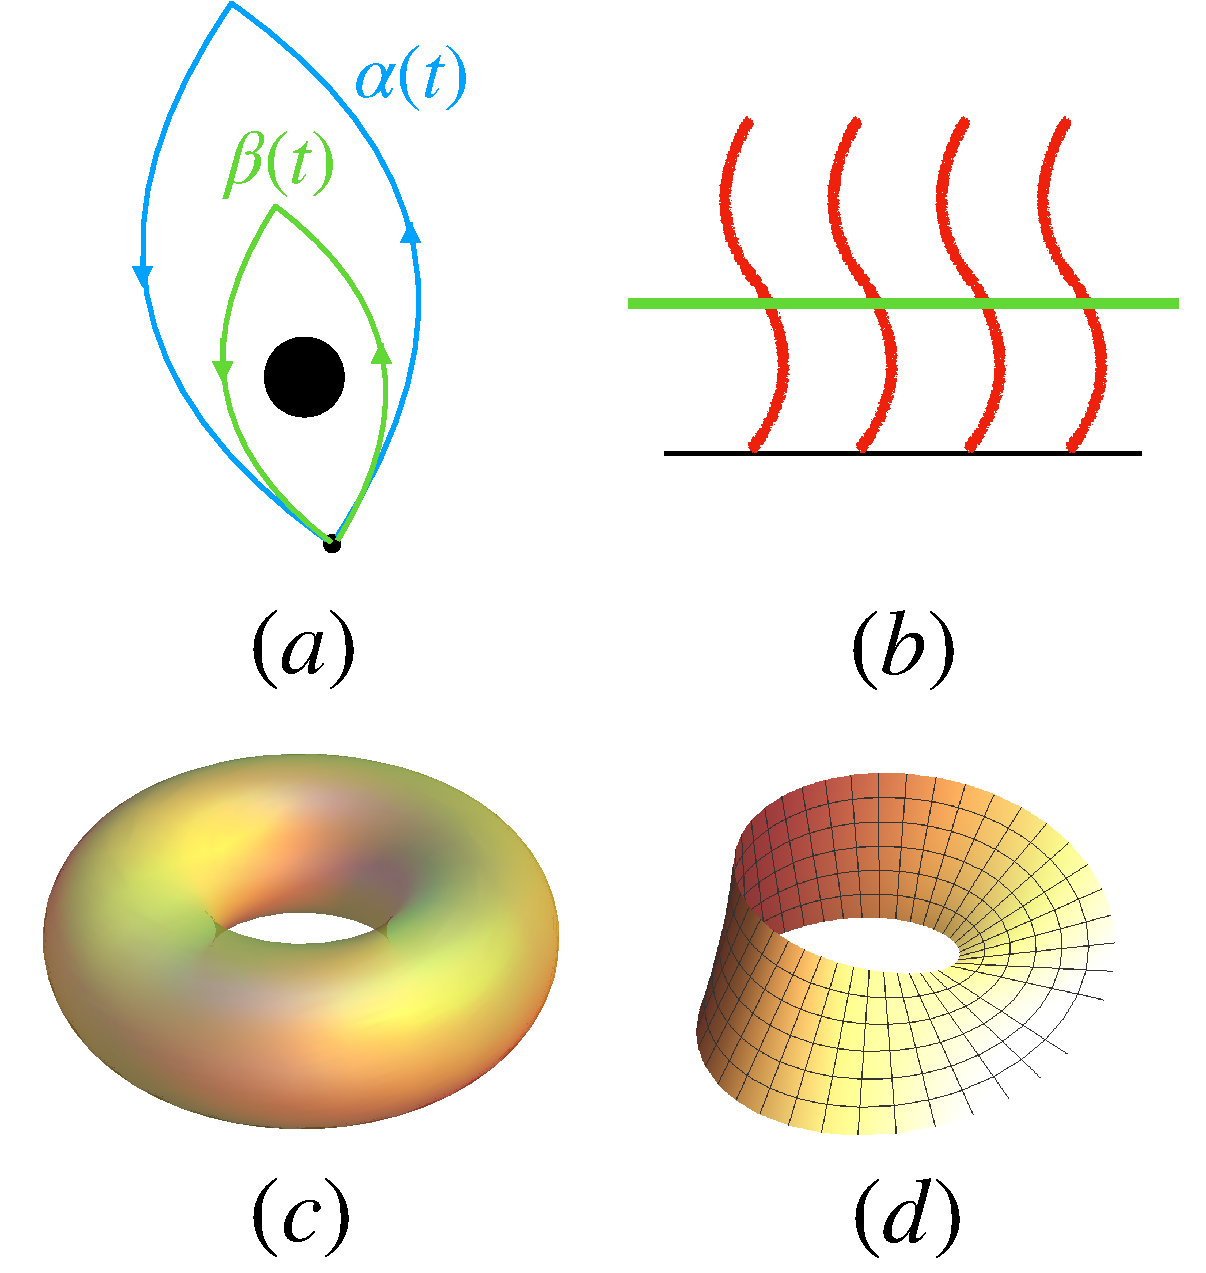
\includegraphics[width=0.7\linewidth]{Figures/topo}
	\caption{使用同伦理论研究的一些对象。(a)经过一个洞,两个同伦等价的圈。(b)一些纤维丛结构和更加复杂的流形也可以作为同伦理论的研究对象。(c)一个甜甜圈面。(d)一个莫比乌斯面。}
	\label{fig:topo}
\end{figure}
	另外,对于向量场$\bv$存不存在$f$使得$\bv = \text{grad }f$呢? 考虑1-形式的外微分:
	\begin{equation}
	d\omega_{\bv}^{1} = \omega_{\text{rot grad }f}^{2} = 0
	\end{equation}
	即$\omega_{\bv}^{1}$应当是闭得,或者说$\text{rot } \bv = 0$,即梯度场是无旋的。但是我们必须注意,尽管对于点电荷$\text{rot } \mathbf{E} = 0$进而$\mathbf{E}=\text{grad } f$但是,
	在无穷长直导线问题中,$\mathbf{j} = 0$的地方$\text{rot } \mathbf{H} = 0$但是不一定存在磁标势。为什么呢?因为导线穿过的一个封闭曲线,不能连续的收缩到一个点。
	
	到此,我们必须讨论,如何刻画空间的这一类性质,即空间有无“洞”的性质了。指的一提的是,同伦理论可以用来研究凝聚态体系中的很多拓扑现象\cite{avron1983homotopy,kennedy2015homotopy}。使用同伦理论可以研究非常多的对象,如图\ref{fig:topo}所示。
	
	\textit{纤维丛理论:}电动力学和量子力学中都有纤维丛理论的应用。事实上,物理学术语,“场”,精确的来说就是纤维丛的截面,局部截面映射确定了规范,而两个局部截面映射之间的变换就能给出了规范势,整个纤维丛可以给出物理理论的规范结构。因此,纤维丛已经深入到了任何和规范对称性相关的物理学理论。在纤维丛理论中,物理学家用到的最多的是主丛\cite{mohajan2015basic},我们考虑的对象如图.\ref{fig:figure}所示。底流形的拓扑、主丛上的模空间$M$\footnote{请参考https://ncatlab.org/nlab/show/moduli+space+of+bundles}的拓扑、和模空间上向量场的拓扑之间有深刻的联系,我们随后在拓扑绝缘体中会简要的看到这一点\cite{avron1983homotopy,kennedy2015homotopy}。本文中应用的纤维丛理论并不是很难,但是建立的图像可以便于我们理解物理理论和数学之间的对应。

	
\begin{figure}
	\centering
	\includegraphics[width=1\linewidth]{Figures/figure}
	\caption{主丛理论中我们研究的几何对象。主丛$P$,结构群$G$和垂直(水平)空间$V_P(H_P)$,底流形$M$和其上的切空间$T_xM$到$H_qP$中的映射。}
	\label{fig:figure}
\end{figure}
	\textit{同调和上同调理论:} 电动力学刚刚的例子,告诉我们恰当形式和闭形式之间有关系,他们集合对应的“商”就能给出来体系洞的信息,正如图.\ref{fig:screenshot002}所示,从这个角度来看,上同调理论对物理学家来说相当的自然。对于同调理论,和同伦理论不同的方式去思考同调理论,那就是通过定义边界链和闭链来区分系统的拓扑性质,直观来说,就是数洞。而这一套对偶的正是恰当形式和闭形式,如图\ref{fig:screenshot003_2}所示。广义的上同调理论,K-理论,在凝聚态体系的拓扑分类中很有用\cite{kitaev2009periodic,kawabata2018symmetry}。
	\begin{figure}
		\centering
		\includegraphics[width=1\linewidth]{Figures/screenshot002}
		\caption{同伦和同调理论研究流形性质的手段。(a)利用同伦等价的圈的思想。(b)利用商去无关边界链的思想。}
		\label{fig:screenshot002}
	\end{figure}
	\begin{figure}
		\centering
		\includegraphics[width=1\linewidth]{Figures/screenshot003}
		\caption{同调群和上同调群的总结。左边:同调群是研究商去无关的边界链。右边:上同调群是研究恰当形式和闭形式对应群的商群。}
		\label{fig:screenshot003_2}
	\end{figure}
    \subsubsection{理论力学}
    我们首先来看看几何知识怎么应用到理论力学中的,随后我们讨论量子力学的时候,也绕不开这些观点。
    
    考虑有$n$个自由度的体系$S$,在理论力学中需要用广义坐标$\{q_i\}$和广义速度$\{\dot{q}_i\}$以及广义动量$\{\dot{p}_i\},p_i = \frac{\partial L}{\partial \dot{q}_i}$描述。定义流形$M$为广义坐标的集合,而状态空间为广义坐标和广义速度的集合,相空间为广义坐标和广义动量的集合。
    
    用数学的语言,考虑流形$M$上的坐标变换$q \to q' = q'(q)$, 我们有:
    \begin{equation}
    \dot{q}'_i= \frac{\partial \dot{q}'_i}{\partial \dot{q}_j} \dot{q}_j
    \end{equation}
    因而,$\dot{q}$实际上是$M$上的逆变向量。对于$p'_i$,我们有:
    \begin{equation}
    p'_i= \frac{\partial \dot{q}_j}{\partial \dot{q}'_i} p_j
    \end{equation}
    因而,$p$实际上是$M$上的协变矢量。
    
    进而,我们知道了:$S$的状态空间为$M$的切丛$TM$,相空间为$M$的余切丛$T^*M$。
    
    $S$的拉格朗日量,是定义在状态空间上的,因而实现了$TM$的向量场,而哈密顿量实现了$T^*M$上的向量场。
    
    考虑任意$2n$维度的$C^\infty$流形$K$上的非退化($i_X \gamma = 0 \to X = 0$)的闭2-形式$\gamma$,辛形式赋予$M$以辛结构,$(K,\gamma)$也称为辛流形。
    
  \textit{$T^*M$上的辛结构:}如果令$dp_i\wedge dq^i$,它给出了一个$T^*M$上的自然的辛结构,  $(T^*M, dp_i\wedge dq^i)$就称为了一个辛流形,$\gamma$作为正则二形式,它显然是恰当的$\gamma = d\theta, \theta = p_i dq^i$。
  
  一个辛结构能够像黎曼结构一样,给出$1-$形式空间和切矢量空间之间的同构。
  
  考虑其上的一个标量场$F(q,p)$,1-形式:
  \begin{equation}
  dF = \frac{\partial F}{\partial q_i}dq^i + \frac{\partial F}{\partial p^i} dp^i
  \end{equation}
    
    现在我们想找到一个场$V_F$使得
    \begin{equation}
    \gamma(U,V_F) = dF(U)
    \end{equation}
    对任意的$U$成立,利用上面定义的$\gamma$,不难求得:
    \begin{equation}
    V_F = \frac{\partial F}{\partial p_i} \hat{\partial}_{q^i} - \frac{\partial F}{\partial q_i} \hat{\partial}_{p_i}
      \end{equation}
      称作$F$对应的流向量场。
      
    如果我们对哈密顿函数取流向量场$V_H$,对比$H = p_i \dot{q}^i - L$就可以得到对应的切向量:
    \begin{equation}
    \dot{q}^i(t) = \frac{\partial H}{\partial p_i} \quad \dot{p}_i(t) = -\frac{\partial H}{\partial q^i}
    \end{equation}
    即是哈密顿方程。

    
    \textit{$TM$上的2-形式} 定义勒让德变换:
    \begin{equation}
    \mathcal{L}(u)(v) = g_x(u,v), u,v \in T_x M
    \end{equation}
    按照定义,有$\mathcal{L}(u) \in T_x^*M$,其中$g$是$M$上的一个度规。例如二次型$T(q,\dot{q}) = \frac{1}{2}g_{i,j}(q)\dot{q}_i \dot{q}_j$中的$g$。
    
    利用这个度规$g$我们能够得到自然的变换$\mathcal{L}: TM \to T^*M$,这个变换将$T^*M$上的辛形式拉回为一个2-形式:$\gamma_L = \mathcal{L} *\gamma$,对应于$(\gamma,H,dH,V_H)$我们在$TM$中就有$(\gamma_L,L,dL,V_L)$,对应于哈密顿方程的$V_L$对应的切向量流正是:
    \begin{equation}
    \frac{d}{dt}\frac{\partial L}{\partial \dot{q}^i} (C) - \frac{\partial L}{\partial q^i}(C) = 0
    \end{equation}
    其中$C$是积分曲线,上面的方程叫做拉格朗日方程。
    
    假设$T$定义了二次型而拉格朗日函数$L = T + V(q)$,那么$TM$上函数$E = T+ V\circ \pi: TM \to R$给出(利用$\partial_{\dot{q}^i}\dot{q}^i = 2T$):
    \begin{equation}
    E(q,\dot{q} ) =2T-[T-V] = T+V
    \end{equation}
    那么$\frac{d}{dt}E = \dot{q}^i \left\{  \frac{d}{dt}\frac{\partial L}{\partial \dot{q}^i})- \frac{\partial L}{\partial q^i}\right\}$
    对于满足了拉格朗日方程的$C$, 有$\frac{d}{dt}E(C) = 0 \to E(C) = \text{const}$,因此$E$也叫做能量函数。
    
    \textit{泊松括号:}我们看到,选取坐标$p,q$对应的哈密顿量天生就有能量的意义,且得到的方程具有简单的形式,回到$T^*M$上,第一个问题是,我们应当如何选取坐标系,使得运动的描述较为简单?下面我们定义泊松括号来探讨这个问题。
    
    
    我们将两个0次形式$f,g$的泊松括号定义成1-形式$df$对$g$对应的向量场$V_g$的作用,即:
    \begin{equation}
    \{f,g\} = df(V_g) = \frac{\partial f}{\partial q^i} \frac{\partial g}{\partial p_i} - f \leftrightarrow g
    \end{equation}
    第二个等式默认我们建立了坐标$(q^i,p_i)$. 如果令$x^\alpha = (q^i,p_i)$,有:
    \begin{equation}
    J_{\alpha,\beta}  = \{x^\alpha,x^\beta\}
    \end{equation}
   计算可以得到:
   \begin{equation}
   J = \left(\begin{array}{cc}
   0_n & I_n \\ 
   -I_n & 0_n
   \end{array} \right)
   \end{equation} 
   这个定义一直是满足的,只要我们对于0形式$U,F$有$dF(U) =\gamma(U,V_F)$,也就是需要辛形式$\gamma$不变。
   
   利用$J$,泊松括号更加容易的可以写作:
   \begin{equation}
   \{f,g\} = J_{\alpha,\beta} \frac{\partial f}{\partial x^\alpha}\frac{\partial g}{\partial x^\beta}
   \end{equation}
   
   
   假设另一个坐标为$X^\alpha = (Q^i,P_i)$如果保证动力学方程最简单,那么就应当有$\gamma = dp_i \wedge dq^i = dP_i \wedge dQ^i$,即保持辛形式不变,或者说是一个\textbf{辛变换},1-形式$\psi = p_idq^i, \phi=P_idQ^i$应当满足$\gamma = d\psi = d\phi$。由Poincare定理我们知道: $\psi - \phi$是局部恰当的,意味着存在0-形式满足$dS = \psi -\phi$这就是我们在力学中学习正则变换的母函数的几何意义。
   
   下面我们来考察辛变换$x^\alpha \to X^\alpha$的充要条件,利用$x^\alpha, X^\alpha$表出$\gamma$有:
   \begin{equation}
   \gamma = \frac{1}{2}J_{\alpha,\beta}dx^\alpha \wedge dx^\beta = \frac{1}{2}J_{\alpha,\beta} dX^\alpha \wedge X^\beta 
   \end{equation}
   $J$应当按照如下式子变换:
   \begin{equation}
   J_{\alpha,\beta} = \frac{\partial X^\mu}{\partial x^\alpha} J_{\mu,\nu}\frac{\partial X^\nu}{\partial x^\beta} 
   \end{equation}
   即$J = U^T J U$,其中$U$为雅克比行列式,满足$U = (\frac{\partial x^\mu}{\partial x^\beta})$
   
   在辛变换下容易证明:
   \begin{equation}
   \{f,g\}(P,Q) = \{f,g\}(p,q)
   \end{equation}
   因此辛变换的另一个充要的定义是保证泊松括号不变。
   
   因此,一个变换是辛变换我们有几个视角:
  \begin{enumerate}
  	\item 保持辛形式不变(没有操作性)。
  	\item 满足矩阵条件$J = U^T J U$即$J$是辛群元素。
  	\item 保持泊松括号不变。
  	\item 新坐标依然是正则坐标。
  \end{enumerate}
   四个条件都告诉我们,辛变换保持正则方程
   \begin{equation}
   \frac{df}{dt} =\{f,H\}
   \end{equation}
   不变。
   
   最显然的辛变换其实就是哈密顿流对应的辛变换。这是考虑不同时刻直接的坐标变换$U^t x^\alpha(t_0) = U^t x^\alpha(t_0 + t)$给出的$U: T^*M \to T^*M$,这显然是一个辛变换,我们来证明一下。
   
   定义其诱导的拉回为$g^*$。对于辛形式$\gamma$我们首先有stokes公式,选取$V$为沿着$V_H$的流线即哈密顿方程的解:
   \begin{equation}
   \int_{\partial V} \psi = \int_V d\psi = \int_V \gamma =0
   \end{equation}
   最后一个等式是因为$\int_V \gamma(V_H,U)  = 0$,进而我们得到:
   \begin{equation}
   \int_C \psi = \int_{gC} \psi \quad \int_V \gamma = \int {gV} \gamma
   \end{equation}
  拉回
   \begin{equation}
   \int_V g^* \gamma = \int_{gV} \gamma=\int_{V} \gamma
   \end{equation}
   意味着$\gamma = g^* \gamma$即哈密顿流也是一个辛变换。
   
   如果考虑哈密顿含有时间$H(p,q,t)$,切触流形$T^*M \times R$:$\psi = p_idq^i - Hdt$,相似的讨论容易给出:
   
   $\oint_C \psi = \oint_{gC} \psi$是一个不变量,而对于$t = \text{const}$即绝热线上的$gC$有,即使含时情况下:
   \begin{equation}
   \oint_C p_i dq^i = \oint_{gC} p_i dq^i 
   \end{equation}
   且能推广到一般的正则变换,即:
   \begin{equation}
   I = \int_C p_i dq^i = \int_{C} P_i dQ^i 
   \end{equation}
   如果考虑的这个哈密顿流是推广的切触流形上的哈密顿流,由于这个等式是定义在绝热线上的,那么这个不变量也就是绝热不变量。
    \subsubsection{电动力学}
    电动力学以其复杂的数学表现形式著称,我们接下来会看到电动力学用几何的语言非常的自然,而纤维丛理论更是能给出其拓扑上的意义。接下来讨论电动力学,电动力学是研究电磁场在时间、空间中的行为,即研究麦克斯韦方程:
    \begin{equation}
    \begin{aligned}
    \nabla \cdot \vec{E} &= \rho/\epsilon_0\\
    \nabla \times \vec{E} &= -\partial_t \vec{B}\\
    \nabla \cdot \vec{B} &= 0\\
    \nabla \times \vec{B} &= -\mu_0 \vec{J} + \mu_0 \epsilon_0 \partial_t \vec{E}
    \end{aligned}
    \end{equation}
    引入矢势和标势,
    \begin{equation}
    \begin{aligned}
    \vec{B} = \nabla \times \vec{A}\\
    \vec{E} = - \nabla \varphi - \partial_t \vec{A}
    \end{aligned}
    \end{equation}
        
    利用几何的知识,电动力学会以一个更加简单的结构展示在我们眼前,仅仅从电荷守恒定律就可以导出一系列的运动方程、和场的性质等等。
    
    定义流形:
   	\begin{equation}
   	R^4 = \{(x^\mu), \mu = 1,2,3,4| x^\mu \in R\}
   	\end{equation}
记$(t,x,y,z) = (x^0,x^1,x^2,x^3)$,并取度规:
\begin{equation}
g = dt^2 - dx^2 - dy^2 - dz^2
\end{equation}    
对向量场的作用为:
\begin{equation}
g(\hat{\partial}_i, \hat{\partial}_j) = \text{diag}(1,-1,-1,-1)
\end{equation}
也就是$\hat{\partial}_\mu$为闵科夫斯基流形$(R^4,g)$上的正交归一基,其上的位置逆变矢量为:
\begin{equation}
X = x^\mu \hat{\partial}_\mu
\end{equation}
1-形式:
\begin{equation}
\omega = x_\mu dx^\mu
\end{equation}
其中$x_\mu = g_{\mu \nu} x_\nu$。

现在定义电流矢量,$J = (j^\mu) = (\rho,\vec{J})$和矢势,$A = (A^\mu) = (\phi,\vec{A})$,等号后面的$\rho,\vec{J},\varphi,\vec{A}$为通常电磁场的电荷密度,电流,电势,和矢势。

电磁场张量:
\begin{equation}
F_{\mu,\nu} = \left(\begin{array}{cccc}
0 & -E_1 & -E_2 & -E_3 \\ 
E_1 & 0 & B_3 & -B_2 \\ 
E_2 & B_3 & 0 & B_1 \\ 
E_3 & B_2 & -B_1 & 0
\end{array} \right)
\end{equation}
注意,在规范变换$A_mu \to A'_\mu + \partial_\mu \Lambda$下,$E$和$B$也就是$F_{\mu,\nu}$都不变,这似乎就蕴含了几何的特征。加上我们正是从电动力学出发讨论同调理论,这一动机更让我们想到麦克斯韦方程的深刻几何内涵。

这些场量,对应在闵科夫斯基流形的矢量场分别为:
\begin{equation}
\mathcal{J} = j_\mu dx^\mu, \mathcal{F} = \frac{1}{2}F_{\mu\nu} dx^\mu dx^\nu
\end{equation}
我们发现
\begin{equation}
d\mathcal{F} = \frac{1}{2} \partial_\rho F_{\mu,\nu} dx^\mu dx^\nu dx^\rho = 0
\end{equation}
恰好给出了两个麦克斯韦方程,而方程:
\begin{equation}
d^\dagger \mathcal{F} = (\nabla \cdot \vec{E}) dx^0 - (\nabla \times \vec{B} - \partial_0 \vec{E}) \cdot (dx^i) = \mathcal{J}
\end{equation}
给出了另外两个麦克斯韦方程,且:
\begin{equation}
(d^\dagger)^2 \mathcal{F} = 0 = d^\dagger \mathcal{J} = \partial_\mu J^\mu = 0
\end{equation}
恰好给出了连续性方程。

麦克斯韦方程现在就可以在任何的坐标系中都有如下的形式:
\begin{equation}
\begin{aligned}
 d\mathcal{F} &= 0\\
d^\dagger \mathcal{F} &= \mathcal{J}
\end{aligned}
\end{equation}

我们还可以使用附录中纤维丛的语言来诠释电动力学,考虑电磁理论是$U(1)$理论,对于$U(1)$丛的一次形式$\omega$,场量:
\begin{equation}
F = - iD^\omega \omega = -i \Omega
\end{equation}
局部截面$\sigma_U: U \to P$对$F$的作用满足:
\begin{equation}
F_U = \sigma^*_U F = -i(d\omega_U + \frac{1}{2}[\omega_U, \omega_U])
\end{equation}
由于$U(1)$是阿贝尔群,我们就有更简单的:
\begin{equation}
F_U = -id\omega_U = -dA_U \in \Lambda^2(U)
\end{equation}
按照上面的定义,令$A_U = A_{U_\mu} dx^\mu$立即有:
\begin{equation}
F_U = \frac{1}{2}(\partial_\mu A_{U_\mu} -\partial_\nu A_{U_\nu}) dx^\mu dx^\nu
\end{equation}
看起来已经和电磁场的结构很相近了。但是,
这也就是说$F_U$就是在$\sigma_U$局部意义下的电磁场,我们自然的想将局部定义的$F_U$粘合成一个真正的电磁场,这样可以不可以呢?考虑两个不同的邻域$U,V$和$\sigma_U :U\to P, \sigma_V: V\to P$我们有,由于$U(1)$群是阿贝尔群,$g_{UV}^{-1}dg_{UV}$是一个恰当形式,因此在$U \cap V$上:
\begin{equation}
F_V = -dA_V = -id(g_{UV}^{-1}dg_{UV}+\omega_U) = -id\omega_U =F_U
\end{equation}
因此我们将局部定义的场宽展到了$M^4$上,也就是只需要令刚刚的$\mathcal{F} = F_U$就可以了。

现在,我们立即看出Bianchi恒等式就是:
\begin{equation}
d\mathcal{F} = d(-dA_U) = -id\Omega_U = 0
\end{equation}

$g_{UV}^{-1}dg_{UV}$的恰当性很重要。在拓扑绝缘体中,它不再恰当或者在某些约束下恰当,我们依此可以得到一些拓扑绝缘体的拓扑数作为拓扑分类。

	\subsection{量子相对论和量子几何学: $CP(n)$作为例子\label{sub2}}	
	这一小节我们专门讨论近年来在数学物理方面,有关量子力学的新进展——对量子态的几何描述,由我们在广义相对论中使用微分几何的经验,通过三条量子力学的公设出发,容易从中构造出相应的辛形式和黎曼度规\cite{minic2004general,provost1980riemannian},随后我们会看到,这样的几何描述深刻的体现在少体物理在外界参数驱动下的性质,也会看到拓扑绝缘体、拓扑超导体和这样的几何描述的关联。
	
	
	\subsubsection{Fubini-Study度规和曲率2-形式}
	在刚建立量子力学理论之时,玻尔曾经论述,“物理现象是在不同的仪器上测量得到的。”这种情况和相对论中的参考系的概念非常接近,Jammer随后论述到\cite{jammer1974philosophy},“就像在相对论中,选择不同的参考系会影响特定的测量,在量子力学中选择不同的实验设备也会作用于测量,因为它决定了我们观测什么。”然而,即便我们有一定的能力选择特定的测量,我们也无法准确地选择测量值,因为量子力学具有内在的随机性。基于上面的两个说法,我们来思考,能够描述量子力学相空间的理论应该伴随什么样的结构。
	\begin{enumerate}
		\item 首先,\textbf{量子力学中的物理定律在不同的测量仪器的选择中应该具有不变性。}
		
	   上面的假设直接的结果就是量子力学应该有内在的辛结构。我们可以考虑下面的思想实验,考虑两个系统,一个经典系统是测量设备,在这个经典系统上我们读取经典的数据并统计他们,那么这个经典系统伴随一个哈密顿量,而被测量的系统也有一个经典哈密顿量,加上两者之间的耦合,整个构成了一个完整的力学体系,整个测量过程就由系统之间的耦合决定。这个完整的经典力学体系自然的伴随了一个良定义的辛结构。按照对应原理,量子力学的某些极限应该给出经典力学,因此我们断言,上面的假设给定了一个量子力学相空间中的闭辛2-形式\cite{brody2001geometric}。
	   
	   \item  \textbf{量子力学具有内在的统计性。}
	   
	   这个假设,也被称作概率统计诠释,给出了量子力学的一个概率论描述。而两个概率事件之间的距离,可以用著名的Fisher距离定义,其上承载了一个自然的黎曼度规,类似下式:
	   \begin{equation}
	   ds^2= \sum_i \frac{dp_i^2}{p_i} = \sum_i dX_i dX_i
	   \end{equation}
	   我们断言,上面的假设给定了一个量子力学相空间中的黎曼度规,准确的说是Fubini-Study度规。
	   
	   \item \textbf{主宰量子力学运动的哈密顿算符的期待值具有能量的意义。}
	   
	   仅仅上面两点还不够决定量子力学的动力学过程,例如我们可以构造$\mathcal{PT}$对称的量子力学\cite{bender1999pt},或者Weinberg非线性非幺正的量子力学\cite{polchinski1991weinberg,weinberg1989testing}。但如果增添这一个假设,那么哈密顿算符的运动也可以用一个Killing 流描述,这样我们可以得到普遍的线性、幺正演化。
	   
		
	\end{enumerate}
	
	
	
	我们现在来从一个简单例子出发,计算量子力学中的内积$\bracket{\cdot}{\cdot}$诱导出的几何结构。考虑依赖一组参数的希尔伯特空间,$\mathcal{H}(s), s = (s_1,\ldots,s_n) \in R^n$,投影$\pi^{-1}: R^n \to \mathcal{H}$。希尔伯特空间上配备了内积$\bracket{\cdot}{\cdot}: \mathcal{H} \times \mathcal{H} \to C$和距离$||\cdot||: \mathcal{H} \to C$,容易计算态$\psi(s + ds)$和$\psi(s)$之间的距离满足:
	\begin{equation}
	||\psi(s+ds) - \psi(s)||^2 = \bracket{\psi(s+ds)-\psi(s)}{\psi(s+ds)-\psi(s)}
	\end{equation}
	到二阶有:
	\begin{equation}
		||\psi(s+ds) - \psi(s)||^2 = \bracket{\partial_i \psi}{\partial_j \psi} ds_i ds_j + O(ds^2)
	\end{equation}
	其中$\partial_i \equiv \frac{\partial}{\partial s_i}$,现在关键是如何理解$ \bracket{\partial_i \psi}{\partial_j \psi} \equiv K_{i,j}$, 容易观察到$K_{i,j} = K^*_{j,i}$,将其实部和虚部分离,
	\begin{equation}
	K_{i,j} = \gamma_{i,j} + i \sigma_{i,j}
	\end{equation}
	分别给出了对称部分和反对称部分,i.e,
	\begin{equation}
	\gamma_{i,j} = \gamma_{j,i}, \quad \sigma_{i,j} = -\sigma_{j,i}
	\end{equation}
	我们来一个一个分析,首先定义2-形式$\sigma = \sigma_{i,j} ds_i\wedge ds_j$容易验证它的它是闭2-形式:
	\begin{enumerate}
		\item $d\sigma = 0$
		\item 存在1-形式$\beta = \beta_i ds_i$其中$\beta_j = -i \bracket{\psi(s)}{\partial_j \psi(s)}$使得$\sigma = d\beta $
	\end{enumerate}

量子力学的一个重要性质是,规范变换不改变任何物理的量,也就是,对于良定义的张量,在$\psi \to e^{i\alpha(s)}\psi$变换下保持不变,其中$\alpha$是一个0-形式。

很显然,在上面变换下$\beta \to \beta + d\alpha$,因此$\sigma = d\beta \to \sigma$是不变的,因此我们给出了一个良定义的辛形式。

不幸的是,在上面的变换下,
\begin{equation}
\gamma'_{i,j} = \gamma_{i,j} + \beta_i \partial_j \alpha + \beta_j \partial_i \alpha + (\partial_i \alpha)(\partial_j \alpha) 
\end{equation}
说明$\gamma_{i,j}$不是一个量子力学语境下良定义的张量的分量,现在问题归结于怎么从$\gamma$出发定出一个张量了,经过一段试验,我们可以得到:
\begin{equation}
g_{i,j} = \gamma_{i,j} - \beta_i \beta_j
\end{equation}
现在可以验证$g_{i,j}$就像张量一样变换了。事实上他就是我们要找的度规,因为定义概率距离:
\begin{equation}
dl^2=  = g_{i,j} ds_i ds_j = \bracket{\delta \psi}{\delta \psi} - |\bracket{\psi}{\delta \psi}|
\end{equation}
其中$\delta \psi = \psi(s+ds) - \psi(s-ds)$,由施瓦兹不等于容易看到$dl^2 \ge 0$且等号取到$\delta \psi =0$即$\ket{\psi(s + ds)}$和$\ket{\psi(s)}$重合的时候。即这样定义的度规满足正定性。

这样,我们就得到了量子力学上的Fubini-Study度规$g$,以及一个辛2形式$\sigma$。

我们还有更加简单的办法推导在规范变换下不变的Fubini-Study度规,去考虑投影希尔伯特空间,i.e,将$e^{i\alpha(s)}\ket{\psi}$对于任意的标量$\alpha(s)$视作同一矢量,相当于内禀了这个规范结构,这样的投影操作使得量子U(1)主丛结构对应的结构群商去了一个$U(1)$。这样定义的态矢量不妨称作$\ket{\tilde{\psi}}$。

新定义的投影希尔伯特空间中的距离$D(\psi_1,\psi_2)$和规范选取$\alpha_{1,2}$无关,将其定义为:
\begin{equation}
D^2(\tilde{\psi}_1,\tilde{\psi}_2) = \inf_{\alpha_1,\alpha_2}||\ket{\psi_1} - \ket{\psi_2}||^2 = 2 - 2|\bracket{\psi_1}{\psi_2}|
\end{equation}
容易看到,这样在射影空间定义的距离对应的度规正是$g_{i,j}$:
\begin{equation}
D^2(\tilde{\psi}(s+ds),\tilde{\psi}(s))  = g_{i,j} ds_i ds_j
\end{equation}

我们来看到一个例子。 考虑谐振子$H = \omega_0 a^\dagger a$的相干态:
\begin{equation}
\ket{\alpha} = D(\alpha) \ket{0}, \quad D(\alpha) = e^{\alpha a - \alpha^* a^\dagger}
\end{equation}
我们有:
\begin{equation}
\ket{\alpha} = \exp(-\frac{1}{2} |\alpha|^2) \sum_0^{\infty} \frac{\alpha^n}{(n!)^{1/2}} \ket{n}
\end{equation}
其中$\alpha = \alpha_1 + i\alpha_2  = \rho e^{i\phi}\in C,$

我们可以简单的计算出内积:
\begin{equation}
\bracket{\alpha}{\alpha'} = \exp{(\bar{\alpha} \alpha' - \frac{1}{2} |\alpha|^2 - \frac{1}{2}|\alpha'^2|)}
\end{equation}
内积诱导出了其上的几何度量:
\begin{equation}
\label{eq:2-form}
\begin{aligned}
dl^2= d\alpha_1^2 + d\alpha_2^2 = d\rho^2 + \rho^2 d\phi^2\\
\sigma = 2 d\alpha_1 \wedge d\alpha_2 = 2 \rho d\rho \wedge d\phi
\end{aligned}
\end{equation}
这恰好是2维平面的度规和辛结构!这样的空间是平直的,因此非常好计算,从而成为了我们一般讨论的出发点。

\subsubsection{基态流形的拓扑和参数测地线方程\label{subsub2}}
\begin{figure}
	\centering
	\includegraphics[width=0.7\linewidth]{Figures/screenshot004}
	\caption{参数依赖的哈密顿量作用在一个 选定了基矢量(投影)的希尔伯特空间上。}
	\label{fig:screenshot004}
\end{figure}


我们考虑体系的哈密顿量是依赖参数的,即$H(s), s = (s_1,\cdots,s_m) \in M$, 这样的哈密顿量的基态问题自然定义了一组态矢量,设其基态为$\ket{0(s)}$,其上的度规结构为$g_{\alpha,\beta}, \alpha,\beta = \{1,2,\cdots,m\}$。研究这样的基态几何的动机在于,凝聚态系统中基态非平凡的拓扑或者几何,对应某些特殊的序,所谓的序就是和体系对称性相关的量,可以用来标志体系所处的相。但是,现在让我们来用几何的办法来定义一些特征量,我们主要考虑$m=2$的情况,但是这容易推广到偶数维度:

首先是(第一)陈数,这和辛结构有关,定义为:
\begin{equation}
C_1 =\frac{1}{2\pi} \int_S \sigma
\end{equation}
注意$S$,按照陈数的定义,必须是封闭的。

我们还可以从黎曼度规出发定义欧拉不变量,先定义
\begin{equation}
\begin{aligned}
g &= \det(g_{\alpha,\beta})\\
\Gamma_{ij}^k &= \frac{1}{2}g^{km}(g_{im,j}+g_{jm,i} - g_{ij,m})\\
\end{aligned}
\end{equation}
和不变距离$ds^2 = Eds_1^2 + 2Fds_1ds_2 + Gds_2^2$,
我们可以得到欧拉示性数:
\begin{equation}
\chi(S) = \frac{1}{2\pi}[\int_S MdS + \oint_{\partial S}k_gdl]
\end{equation}
其中(确定坐标)
\begin{equation}
\begin{aligned}
K& = g^{-1/2}[\partial_2 (g^{1/2} \Gamma_{11}^2/E) - \partial_1(g^{1/2}\Gamma_{12}^2 /E)]\\
k_g &= g^{1/2}G^{-3/2}\Gamma_{22}^1\\
dS &= g^{1/2} ds_1ds_2\\
dl &= G^{1/2}ds_2
\end{aligned}
\end{equation}

下面看到一个例子。考虑一个二能级系统,
\begin{equation}
H = \epsilon(k)\sigma_0 + \mathbf{d}(k) \cdot \bm{\sigma} 
\end{equation}
首先取$ k = (\theta,\phi)$ 以及 $\mathbf{d} = |d|(\sin(\theta)\cos(\phi), sin(\theta)\sin(\phi), \cos(\theta) \equiv \mathbf{n}$,本征能量就是 $\epsilon = \pm \frac{1}{2} |d|$:
\begin{equation}
\ket{k, -} = \left(\begin{array}{c}
\sin(\frac{\theta}{2})e^{-i\phi} \\ 
-\cos(\frac{\theta}{2})
\end{array} \right) \quad \ket{k, +} = \left(\begin{array}{c}
\cos(\frac{\theta}{2})e^{-i\phi} \\ 
\sin(\frac{\theta}{2})
\end{array} \right)
\end{equation}
对应的$A$就是$\ket{-,k}$:
\begin{equation}
A_\theta = i\bra{-,k} \partial_\theta \ket{-,k} = 0, A_\phi = i\bra{-,k}\partial_\phi \ket{-,k} = \sin(\theta/2)^2
\end{equation}
其中$A_{|d|}$不存在。 

曲率可以计算得到:
\begin{equation}
B_{\theta,\phi} = \partial_\theta A_\phi - \partial_\phi A_\theta = \frac{\sin(\theta)}{2}
\end{equation}
可见它确实是规范不变的,
将$B_{\mu \nu}$ 作为二形式,这个量就和坐标变换无关
\begin{equation}
B_{\mu \nu} d\mu \wedge d\mu = B_{\theta,\phi} d\theta \wedge d\phi = B_{k_i,k_j} dk_i \wedge dk_j
\end{equation}
其中 $k$ 用 $\mathbf{k} = \mathbf{n(\theta,\phi)}$ 或者 $\mathbf{k} = (k_x,k_y,k_z)$来刻画,相当于将$(\theta,\phi)$嵌入了一个三维的坐标系中,它恰好是一个求,可以计算
\begin{equation}
B_{k_i,k_j} = B_{\theta,\phi} \frac{\partial(\theta,\phi)}{\partial(k_i,k_j)}
\end{equation}
$A_{|d|}$不存在,因此很好计算 :
\begin{equation}
\mathcal{B} = \nabla \times A = \epsilon_{i,j,k}B_{k_i,k_j} = \frac{\vec{k}}{|k|^3} 
\end{equation}
可见,自旋1/2的2形式类似参数空间中的磁场。这和我们在上一节$U(1)$主丛的数学结构类似。

上面的嵌入之后的流形是一个球,其上的高斯张量容易计算为$K = 4$,且欧拉不变量可以计算为:
\begin{equation}
\chi = 2
\end{equation}

推广到自旋$S$显然$\chi$不变,而陈数变为$C = 2S$。

除了上面讲到的拓扑特性,对于$s = s(t)$我们还可以从薛定谔方程导出参数测地线方程:
\begin{equation}
\ddot{s}^\mu + \Gamma_{\alpha,\beta}^\mu \dot{s}^\alpha \dot{s}^\beta = 0
\end{equation}
它给出了我们能够对系统控制的程度,也就是不发生简并,从一个参数点到达另一个参数点的最短路径。
	\subsubsection{可观测量和几何薛定谔方程}
	在上面我们的讨论并没有涉及量子力学的任何动力学,我们来考虑构造一下动力学。现在我们不能再取代表元素$\ket{\psi(s)}$去讨论了,我们首先需要一个$\mathcal{H} = C^n$上的坐标,例如$\ket{\psi} = \sum_\alpha \psi_{\alpha} \ket{e_\alpha(s)}$其中$e_\alpha(s)$是基,我们这里先假设$e_\alpha(s)$是自然选取的,而不一定是哈密顿量的本征态。记$\mathcal{H}$上配备度规的Kähler空间为$\mathcal{P}(\mathcal{H})$,其上配备的二形式,按照式.\ref{eq:2-form}暗示的,取:
\begin{equation}
\omega = dp_\alpha \wedge dq^\alpha, q^\alpha = \sqrt{2} \text{Re}(\psi_\alpha) , p^\alpha = \sqrt{2}\text{Im}(\psi_\alpha)
\end{equation}
即对每一个分量都定义了二形式,泊松括号就是:
\begin{equation}
\{f,g\} = (\omega^{-1})^{\alpha \beta}\frac{\partial f}{\partial Q^\alpha}\frac{\partial g}{\partial Q^\beta}
\end{equation}
其中$(\omega^{-1})^{\alpha \beta}$是$\omega$的逆矩阵,而$Q^\alpha = (p_\alpha, q^\alpha
)$是一组正则的坐标集。

我们距离几何薛定谔方程还有一个哈密顿量的距离,考虑玻尔定则告诉我们:
\begin{equation}
1 = \frac{1}{2} \sum_\alpha [(p^\alpha)^2 + (q_\alpha)^2]
\end{equation}

上面的指标升降是一个平坦的度规控制的。我们意识到,如果赋予其概率的意义,可以这样定义哈密顿量:
\begin{equation}
\label{eq:hami}
h = \frac{1}{2} \sum_\alpha [(p^\alpha)^2 + (q_\alpha)^2] \omega_\alpha
\end{equation}
	其中$\omega_\alpha$为某些观测量,事实上,$\omega_{\alpha} - \omega_{\beta}$正是原子物理中介绍的“谱线”所处的位置。
	
	这样,哈密顿方程
	\begin{equation}
	\begin{aligned}
	\frac{dp_\alpha}{dt} = \{h,p_\alpha\} \\
	\frac{dq^\alpha}{dt} = \{h,q^\alpha\}
	\end{aligned}
	\end{equation}
	就给出了坐标的演化,不难验证,上面的定义的恰好就等价于薛定谔方程的分量形式。
	
	利用式子\ref{eq:hami}还可以类似定义可观测量,定义本征值$o_\alpha$为:
	\begin{equation}
	\frac{dO}{dX^\alpha} = o_\alpha \omega_{\alpha,\beta} X^\beta
	\end{equation}
	其中$X^\alpha = (p^\alpha,q^\alpha)$我们就有观测量:$O = \sum_{\alpha,\beta} o_\alpha h_{\alpha,\beta} X^\alpha X^\beta$。
	
	容易验证上面的定义和$dO/dt = \{h,O\}$相容。如果定义底流形上的坐标$s^\alpha$,按照上面的章节我们也可以得到参数满足的测地线方程,但是现在,由于波函数不再是以基态作为坐标,而是任意参数化的,因此体系的测地线方程也不再满足一个简洁的形式了,有兴趣的读者可以继续参考文献\cite{minic2004general}。
	\subsection{拓扑绝缘体\label{sub3}}
	这一节我们来看几何是怎么应用在无相互作用的周期性体系的\footnote{可以参考网站:https://topocondmat.org/, http://www.damtp.cam.ac.uk/user/tong/qhe.html}。
	
	在上一节中,我们介绍了量子力学中自然的几何构造,它揭示了内积作为希尔伯特中的运算$\mathcal{H}\times \mathcal{H} \to C$形成了一个配备了辛形式(曲率二形式,或者说Berry曲率)和一个黎曼度规的Kähler流形。由于不同的相位标记着同一量子态,希尔伯特空间商去一个不重要的相位得到的等价类构成了真实的相空间,也就是射影空间,这样的映射赋予了一个$U(1)$主丛结构。
	
	量子相空间是定义在某些参数流形上的,一个自然的、从多体物理的单体近似中演生出来的就是布里渊区了。我们先来讨论周期性单粒子哈密顿量给出的布里渊区。
	
	考虑希尔伯特空间$\mathcal{H} = \ell^2(Z^d) \times C^n$,其中$\ell^2(Z^d)$代表一个原胞中的$d$个原子,内部自由度(例如轨道、自旋)对应的空间为$C^n$,定义$\ket{r,i} = \ket{r} \times\ket{i}$其中$\ket{r} \in \ell^2(Z^d)$且在对应$r = (r_1,r_2,...,r_n)$的格点上取得振幅,其他为$0$,对应的正交关系:
\begin{equation}
\bracket{r,i}{r',j} = \delta_{r,r'} \delta_{i,j}
\end{equation}	

我们考虑的单粒子哈密顿量都具有\textbf{平移对称性},i,e,
\begin{equation}
[T_x,H] = 0, T_x \ket{r,i} = \ket{r+x,i}
\end{equation}
这样,在单粒子基下有:
\begin{equation}
H \ket{r,i} = \sum_{r',j} t_{j,i}(r')\ket{r+r',j}
\end{equation}
其中$t_{ji}: C^n \to C^n$为相邻原胞的跃迁算符。

如果有一个模型的$\text{card}(r') \le 1$,则称这个模型为紧束缚模型。

离散傅里叶变换:
\begin{equation}
\mathcal{F}: \ket{x,i} \to \ket{k,i}, \ket{k,i} = \frac{1}{\sqrt{V}}\sum_x e^{ikx}\ket{x,i}
\end{equation}
$V$是体系的体积,用来归一化体系的本征向量。
对应的跃迁算符满足:

\begin{equation}
t_x \ket{k,i} = e^{-ikx}\ket{k,i}
\end{equation}
因此:
\begin{equation}
H\ket{k,i} = \sum_j H_{ji}(k)\ket{k,j}
\end{equation}
其中:
\begin{equation}
H(k) = \sum_x \exp(-ikx)h(x)
\end{equation}
也就是,我们按照平移对称性对体系进行了直和分解\begin{equation}
H = \oplus_k H_k
\end{equation}

接下来我们考虑Fock空间,这使得我们可以讨论无相互作用的多粒子问题。假设我们考虑的是费米子,考虑$\mathcal{F} = \wedge(\mathcal{H}) = \oplus_m \wedge^m(\mathcal{H})$其中wedge符号$\wedge$对应构造一个交换反对称的基矢,它们是整个张量空间的子集。

上面具有平移对称性的哈密顿量的一个自然的基矢量为$\ket{k,i}$,那么整个张量空间中的基有:
\begin{equation}
\{ \ket{k_1,i_1}\otimes\ldots \otimes \ket{k_m,i_m} \}
\end{equation}
那么$\mathcal{F}$的基就是:$\{\ket{k_1,i_1}\wedge \ldots \wedge \ket{k_m,i_m}\}$。

我们增加定义$m = 0$时候的希尔伯特空间,其中只有一个矢量$\ket{0}$,那么$\mathcal{F}$上有算符:
\begin{equation}
c_i(k)^\dagger \ket{0} = \ket{k,i}, c_i(k)^\dagger \ket{k,i} = 0
\end{equation}


对应产生一个具有$i$轨道指标的动量为$k$的粒子。$c_i(k)$为$c_i(k^\dagger)$的厄米共轭。

这样,算符满足反对易关系$\{c_i(k),c_j(k')\} = \{c_i(k)^\dagger,c_j(k')^\dagger\}  = 0, \{c_i(k)^\dagger,c_j(k')\} = \delta_{ij} \delta_{k,k'}$

作用在$\mathcal{H}$上的单粒子算符$O$容易扩展定义到$F$上,利用:
\begin{equation}
\hat{O} (\wedge_{k,i} \ket{k,i}) = \wedge_{k,i}(O\ket{k,i})
\end{equation}
得到
\begin{equation}
\hat{O} = \sum_{k,k',i,j} O_{i,j}c_i^{\dagger}(k) c_j(k')
\end{equation}
哈密顿量:
\begin{equation}
H = \sum_{k,i,j}H_{i,j}(k) c_i^\dagger(k) c_j(k)
\end{equation}
在$\ket{k}$中是对角的。

因此,上面的$H_{i,j}$作为$\ket{i}$基下的,含有参数流形$k \in T^d$的意义下,被定义出了。定义$\psi = (c_1(k),\ldots,c_n(k))^T$我们有:
\begin{equation}
H = \psi^\dagger H(k) \psi
\end{equation}
一般我们把$H(k)$叫做Bloch哈密顿量,简称哈密顿量。

考虑$\psi \to U\psi$,其中$U^\dagger H U = \Lambda = \text{diag}(E_1,E_2,\ldots,E_n)$也就是将$H(k)$相似变化为对角阵的相似变换,其列对应着单粒子波函数,而$E_i(k)$也叫作能带,以体系的能带能量大小进行编号$i<j$则$E_i \le E_j$,填充每一个$i$之后,如果$E_i \l E_{i+1}$那么我们称体系是一个绝缘体,也叫做有能隙的。下面来看一个例子。

考虑下面的哈密顿量(SSH模型\cite{su1979solitons}\footnote{参考下面的网页笔记:https://phyx.readthedocs.io/en/latest/TI/Lecture\%20notes/1.html}),
\begin{equation}
H=\sum_{n=1}^N(v_n c_{n,1}^\dagger c_{n,2}+w_nc_{n,2}^\dagger c_{n+1,1}+h.c.) 
\end{equation}
利用 $\mathbf{c}_n^\dagger=(c_{n,1}^\dagger,c_{n,2}^\dagger)=(c_{2n-1}^\dagger,c_{2n}^\dagger)$ 我们有:
\begin{equation}
H=\sum_{m,n=1}^N \mathbf{c}_m^\dagger H_{mn}\mathbf{c}_n
\end{equation}

\begin{equation}
\begin{split}\hat{H}=\begin{pmatrix}\mathbf{c}_1^\dagger&\mathbf{c}_2^\dagger&\cdots&\mathbf{c}_N^\dagger \end{pmatrix}
\begin{pmatrix} U & T &0 & \cdots&T^\dagger\\
T^\dagger &U&T&\cdots&0\\
0&T^\dagger&U&\cdots&0\\
\vdots&\vdots&\vdots&\vdots&\vdots\\
T&0&0&T^\dagger&U
\end{pmatrix}
\begin{pmatrix}\mathbf{c}_1\\\mathbf{c}_2\\\vdots\\\mathbf{c}_N\end{pmatrix}\end{split}
\end{equation}
利用傅里叶变换:
\begin{equation}
\begin{split}\Rightarrow \begin{pmatrix}\mathbf{c}_1^\dagger&\mathbf{c}_1^\dagger e^{-ikb}&\cdots&\mathbf{c}_1^\dagger e^{-ik(N-1)b} \end{pmatrix}
\begin{pmatrix} U & T &0 & \cdots&T^\dagger\\
T^\dagger &U&T&\cdots&0\\
0&T^\dagger&U&\cdots&0\\
\vdots&\vdots&\vdots&\vdots&\vdots\\
T&0&0&T^\dagger&U
\end{pmatrix}
\begin{pmatrix}\mathbf{c}_1\\\mathbf{c}_1 e^{ikb}\\\vdots\\\mathbf{c}_1e^{ik(N-1)b}\end{pmatrix}\end{split}
\end{equation}
得到下面的对角的哈密顿量。
\begin{equation}
\begin{split}=\begin{pmatrix}\mathbf{c}_1^\dagger&\cdots&\mathbf{c}_1^\dagger \end{pmatrix}
\begin{pmatrix} U+Te^{ikb}+T^\dagger e^{-ikb} & &\\
&\ddots&\\
&&U+Te^{ikb}+T^\dagger e^{-ikb}
\end{pmatrix}
\begin{pmatrix}\mathbf{c}_1\\\vdots\\\mathbf{c}_1\end{pmatrix}\end{split}
\end{equation}
因此,我们找到了直和分解$H = \oplus_n H(k)$其中 $H(k) = U + Te^{ikb} + h.c. = \mathbf{h}(k) \cdot \sigma$,
上面各个量为
\begin{equation}
\begin{split}h_x(k)=&\text{Re}(v)+|w|\cos(kb+\text{arg}(w))\\
h_y(k)=&-\text{Im}(v)+|w|\sin(kb+\text{arg}(w))\\
h_z(k)=&0\end{split}
\end{equation}
我们先来顺手讨论一下1D模型的拓扑性质来作为前奏,体系能够写作:
\begin{equation}
H(k) = \left(\begin{matrix}
0 &q(k)\\
q^\dagger(k) & 0\\
\end{matrix}\right)
\end{equation}
的原因(即$h_z(k) = 0$)是体系受到Chiral对称性的保护,也就是:
\begin{equation}
\Gamma = \sum_n(c^\dagger_{n,1}c_{n,1} -c^\dagger_{n,2}c_{n,2}), \{\Gamma,H\} = 0
\end{equation}
体系已经写在了$\Gamma$的对角表象下。

我们来考虑体系有没有零本征值,也就是讨论${\det} H =- \det q^\dagger q$,将其视作$C\to S^2$,同伦不变量:
\begin{equation}
v_t = \frac{1}{4\pi i} \int_{-\pi}^{\pi} \Gamma H^{-1} dH = 0
\end{equation}
虽然它是一个拓扑不变量,因为$d(h^{-1}dh) = 0$,1-形式$\mathcal{A} = \Gamma H^{-1} dH = q^{-1} dq - q^{\dagger -1}dq^\dagger$是闭形式,但是由于手征对称性它必然恰当,因而是平庸的$v_t = 0$。

但是如果我们只考虑对称性约束下的拓扑数\cite{asboth2016short},例如:
\begin{equation}
v = \frac{1}{2\pi} \int_{-\pi}^\pi q^{-1}dq
\end{equation}

容易验证这个拓扑不变量的拓扑性质,施加小的微绕$H \to H' = H + \delta H$只要$\delta H$满足对称性,$v$都不会改变。因此它构成了体系的一个拓扑数。

这样的拓扑数有重要的意义,那就是在打破了这个体系的周期性之后,也就是采取了截断边界条件之后,在边缘上的物理往往会因为反常性变得很特殊。例如上面的例子,SSH模型在截断了边界之后会出现零模,见图\ref{fig:figwaveno}。物理上如何理解这样的过程?可以这样想想。考虑一个三维空间,当空间中没有点电荷的时候(也就是没有洞),整个空间是一个无限大的空间还是有一个在物理上是没有影响的。而当有一个孤立的点电荷的时候,体系在自由空间中是球面解,而当空间是$z>0$这个半无限大的空间,并且采取合适边界条件的时候,在边界上就会给出有效的感应电荷分布了,我们还可以用电像法来有效的模拟这个分布。这个激发的有效的电荷分布会剧烈的改变$z = 0$附近的电场。利用这种思路,可以考虑带边界条件情况的流形和上面的粒子场的分布的几何,超出了本文的讨论范围。

也可以这样去想想问题。一个拓扑上平庸的绝缘体和真空等价,截断等效于拼接两个真空在绝缘体的两端,由于两者拓扑等价,波函数可以连续的改变到真空态。而对于拓扑非平庸的绝缘体,波函数不可以连续的改变到真空态必须跨越某种相变点。这个相变点就是简并点,那么在边界上就会有无能隙的边缘态(作为媒介态)了。沿着这个思路,似乎我们需要利用一个正合序列联系不带边和带边的代数,这样去证明体的拓扑数和边缘态的关系需要用到非常非平庸的数学,超出了本文的内容。

\begin{figure}
	\centering
	\includegraphics[width=1\linewidth]{Figures/Fig_wave_no}
	\caption{SSH模型的边缘态和能谱。(a) 有限大的体系在$|w| = |v|$发生拓扑相变。其中$|w|<|v|$的一侧没有零模;而$|w|>|v|$的一侧有零模。(b) 无限大的体系在$|w|=|v|$处发生了能带的简并,也就是$\det(H) = 0\to |w| = |v|$,也可以侧面反映存在拓扑数描述这个现象。(c) 当$w/v = 1.3$时候体系的零模。两个简并的模式局域在两侧。(d)当$w/v = 0.9$时候体系的某两个体态。}
	\label{fig:figwaveno}
\end{figure}

注意到我们上面的拓扑数,只是在对称性考虑下的“半个”拓扑数。后来,X Chen, X.-G Wen等人在此基础上提出了对称性保护的拓扑序(SPT)的概念\cite{wen2013classifying,gu2009tensor,chen2010local},在后面我们也会介绍另一种不受对称性保护的拓扑序(按照Wen等人的定义),即整数量子霍尔效应。 

为了理解整数霍尔效应中拓扑是怎么体现的,我们不妨从一个有能隙的两带系统出发,$k = (k_x,k_y)$:
\begin{equation}
H(k) = \mathbf{a}\cdot \bm{\sigma}
\end{equation}
其中$\mathbf{a}= (a_i), i = {0,1,2,3}$而$\bm{\sigma} = (I_{2\times2}, \vec{\sigma})$。有能隙意味这$\vec{a} \ne 0$。首先注意到$a_0$部分在拓扑意义上不重要,因为我们总可以将其连续的相除(即平移能谱)而不使体系发生相变,将参数空间$k$推至$\vec{a} = (a_i), i = 1,2,3$,同时连续变换也能将$\vec{a}$归一化,物理上实际上是固定了体系的能标,因此$\vec{a} \to \frac{\vec{a}}{|a|}\in S^2$。这实际上是证明了$G_1(C^2) \simeq S^2$,其中,$G_m(C^n)$指的$n$能级系统的$m$个能级被占据了的Grassmannian。

现在我们有$k \in T^2 \to \vec{a} \in S^2$了,用附录中的同伦知识,对于$T^2 \to X$上的分类,首先注意到$\pi_1(T^2) \simeq Z \times Z$, 因此$S^1 \to T^2$有两个基本圈,记做$\gamma_{1,2}$那么$f: T^2 \to X $诱导的$S^1 \to X$的映射就是:
\begin{equation}
f \circ \gamma_i : S^1 \to X
\end{equation}
容易证明映射$f_1: T^2 \to X$, $f_2: T^2 \to X$,只要$f_1 \circ \gamma_i$和$f_1 \circ \gamma_i, i = 1,2$不同伦,那么在上面的意义下$f_1$和$f_2$也不同伦。然而,即使上面的证明使得$\gamma_i$相应的部分是“配对的”, 我们还剩下$S^2 \to X$,因此只用看$\pi_1(X)$的两部分,$\pi_2(X)$的一部分等等,

接下来只需要看
$T^2 \to X = G_1(C^2) \simeq S^2$的一部分,注意到$\pi_1(S^2) = 0$因此要去看$\pi_2(S^2)$了,而容易证明$\pi_2(S^2) = Z$因此$T^2 \to S^2$的映射度和诱导映射$S^2 \to S^2$的一致(实际上是$T^2$上的复线丛的陈数)。它等于:
\begin{equation}
n = \frac{i}{2\pi} \int_{T^2}\bracket{d\psi_0}{d\psi_0}
\end{equation}

类似的思想推广到$T^d$上并不是难事,详见参考文献\cite{avron1983homotopy}, 具体的例子,例如对于Hofstadter模型,可见后面的章节。

我们接下来还要接触一类SPT,即拓扑绝缘体上的量子自旋霍尔效应\cite{RevModPhys.83.1057,qi2010quantum,Kane2005a,sheng2006quantum,Kane2005,Wu2006,culcer2012transport}。拓扑绝缘体拥有被时间反演对称性$\mathcal{T}^2 = -1$保护的边缘态,按照上面的被对称性保护的态,就是说这样的态在输运过程中,任何边界上满足对称性的扰动都不会影响这个态,为了构造一个这样的模型\cite{hasan2011three},我们首先考虑看看这个模型应该具有什么样的特征,首先我们考虑边界上的物理\cite{fukui2008topological},如图.\ref{fig:scatter}所示。

我们把左(L)右(R)的入射的态记做 $\left|n,\textrm{L}\right\rangle$ 和 $\left|n,\textrm{R}\right\rangle$。其中 $n$ 是量子数,从$1$ 到 $N$。 出射的态是入射态的时间反演: $\mathcal{T}\left|n,\textrm{L}\right\rangle$ 和 $\mathcal{T}\left|n,\textrm{R}\right\rangle$。实际的态矢量是出射态和入射态的叠加态:
\begin{figure}
	\centering
	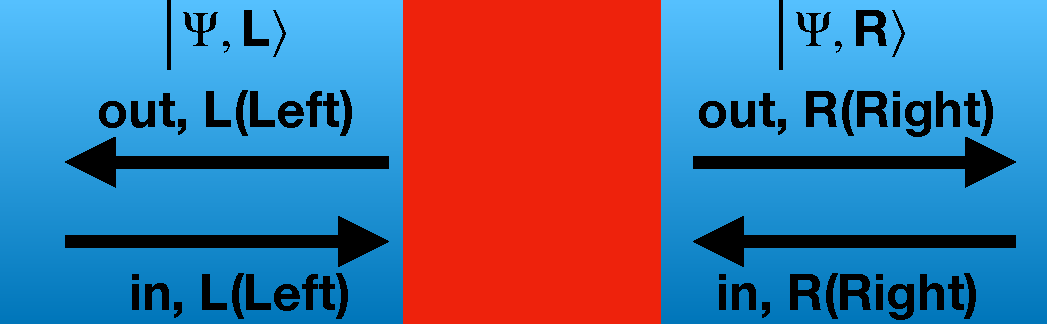
\includegraphics[width=0.7\linewidth]{Figures/scatter}
	\caption{拓扑绝缘体边缘上的散射问题。即中间有一个满足时间反演对称性的微扰区段(红色)和两个传播的区段(蓝色渐变区段),考虑这上面的一个散射问题。}
	\label{fig:scatter}
\end{figure}

\begin{equation}
\begin{aligned}
\left|\Psi,\textrm{L}\right\rangle &= \sum_{n=1}^N \alpha_{n,\textrm{L}}\,\left|n,\textrm{L}\right\rangle + \beta_{n,\textrm{L}}\,\mathcal{T}\left|n,\textrm{L}\right\rangle\,,\\
\left|\Psi,\textrm{R}\right\rangle &= \sum_{n=1}^N \alpha_{n,\textrm{R}}\,\left|n,\textrm{R}\right\rangle + \beta_{n,\textrm{R}}\,\mathcal{T}\left|n,\textrm{R}\right\rangle\,.
\end{aligned}
\end{equation}


如果我们取自然基,那么定义 $\alpha_\textrm{L} = (\alpha_{1,\textrm{L}},\dots,\alpha_{N,\textrm{L}})^T$,扰动的红色区段对于的散射矩阵$S$为 

\begin{equation}
\begin{pmatrix} \beta_\textrm{L} \\ \beta_\textrm{R} \end{pmatrix} = S \begin{pmatrix} \alpha_\textrm{L} \\ \alpha_\textrm{R} \end{pmatrix}.
\end{equation}

因为有$2N$ 入射态 $2N$出射态,因此$S$ 是$2N\times 2N$ 的矩阵。并且$S$ 容易验证是幺正的, $S=S^\dagger$。$S$矩阵按照物理诠释,可以分成四个$N\times N$的块,

$$ S = \begin{pmatrix} r & t\\ t' & r' \end{pmatrix}\,. $$

如果我们能够通过增加满足对称性的扰动消除所有的边缘态,我们就应该能得到 $t = t' = 0$,也就是所有的模式都被散射回去了,因此 $r^\dagger r = r'^\dagger r' = 1$。

这是否可能?我们来看看时间反演对称性对$S$矩阵的约束,

时间反演对称性 $\mathcal{T}$是一个反幺正算符,和哈密顿正对易, $\mathcal{T}^2$ 可能有两种取值 $\mathcal{T}^2=\pm1$ 负号是对于半整数自旋的情况,对于无自旋情况 $\mathcal{T}=\mathcal{K}$ 其中$\mathcal{K}$是复共轭算符。对于半自旋体系,我们有: $\mathcal{T}=i\sigma_y\mathcal{K}$.

考虑:
\begin{equation}
\begin{aligned}
\mathcal{T}\left|\Psi,\textrm{L}\right\rangle &= \sum_{n=1}^N \alpha^*_{n,\textrm{L}}\,\mathcal{T}\left|n,\textrm{L}\right\rangle + \beta^*_{n,\textrm{L}}\,\mathcal{T}^2\left|n,\textrm{L}\right\rangle\,,\\
\mathcal{T}\left|\Psi,\textrm{R}\right\rangle &= \sum_{n=1}^N \alpha^*_{n,\textrm{R}}\,\mathcal{T}\left|n,\textrm{R}\right\rangle + \beta^*_{n,\textrm{R}}\,\mathcal{T}^2\left|n,\textrm{R}\right\rangle\,. 
\end{aligned}
\end{equation}

由于时间反演不改变系统的能量, $\mathcal{T}\left|\Psi,\textrm{R}\right\rangle$ , $\mathcal{T}\left|\Psi,\textrm{L}\right\rangle$和 $\left|\Psi,\textrm{R}\right\rangle$, $\left|\Psi,\textrm{L}\right\rangle$具有同样的能量。因此入射态和散射态的振幅在时间反演下用同样的$S$矩阵描述,但是入射和出射态相互交换了,于是有:

\begin{equation}
S\mathcal{T}^2 \begin{pmatrix}\beta^*_\textrm{L} \\ \beta^*_\textrm{R} \end{pmatrix} = \begin{pmatrix} \alpha^*_\textrm{L} \\ \alpha^*_\textrm{R} \end{pmatrix}\,. 
\end{equation}

两边乘上 $\mathcal{T}^2S^\dagger$ 再取复共轭,给出
\begin{equation}
\begin{pmatrix} \beta_\textrm{L} \\ \beta_\textrm{R} \end{pmatrix} = \mathcal{T}^2\,S^T \begin{pmatrix} \alpha_\textrm{L} \\ \alpha_\textrm{R} \end{pmatrix}. 
\end{equation}
于是我们有:
 \begin{equation}
S = \mathcal{T}^2 S^T. 
\end{equation}

如果$\mathcal{T}^2=1$, 散射矩阵就是对称的 ($S=S^T$);如果 $\mathcal{T}^2=-1$,那么散射矩阵是反对称的 ($S=-S^T$).

对于 $t=t'=0$,完全散射的情况下,
如果 $S=S^T$,时间反演对称性不能给出新的结果。但是如果$S=-S^T$ 以及 $t=t'=0$, 那么$N\times N$ 反射矩阵$r$也是幺正的 $r^\dagger r=1$, 而且还是反对称的 $r=-r^T$.

如果 $N$ 是奇数, 那么就会得出矛盾:任何偶数维度的反对称矩阵必须有一个零本征值,即行列式为0,而幺正矩阵的本征值必须是$1$的某个根,也就是本征值为$1$!

这立刻告诉我们,在$N$为奇数,$\mathcal{T}^2 = -1$必须存在一个通道不被散射。这样的有能隙的体态,可以看成两个相互时间反演的Chern数分类的绝缘体通过不关闭能隙的、满足时间反演不变性的耦合得到:
\begin{equation}
H_{\mathcal{Z}_2} = \left(\begin{array}{cc}
H(k) & g(k) \\ 
g^\dagger(k) & \mathcal{T}^{-1}H(k)\mathcal{T}
\end{array} \right)
\end{equation}

Fu和Kane (Topological insulators with inversion symmetry)最先提出如何计算这一类系统的拓扑数:
\begin{equation}
D = \frac{1}{2\pi} [\oint_{\partial \text{EBZ}} \mathcal{A} - \int_{\text{EBZ}} \mathcal{F} ] \text{mod } 2
\end{equation}
其中EBZ是半个布里渊区(配合合适的边界条件),$\mathcal{A}$是Berry联络(1-形式),$\mathcal{F}$是对应的Berry曲率(2-形式),注意EBZ是一个带边的流形1-形式不是规范不变的,2-形式的积分也不是整数。正确的理解是,考虑$\text{EBZ} \to H_{\mathcal{Z}_2}$的映射$g$,利用Wess-Zumino办法将$EBZ$延拓到一个球面上(准确的说是南北极互为反演对的球面),见参考文献\cite{fukui2008topological,moore2007topological}。

对拓扑绝缘体、陈绝缘体的介绍是为后面的量子模拟做准备的,现在的知识已经足够理解后面的计算了。

	\newpage
   \section{超导量子电路}
   超导量子电路是一种人工量子材料。\cite{you2003quantum,GU20171}过去20年里,超导量子电路在理论和实验上取得了极大的成功,不仅仅为我们提供了一个量子计算的想象空间,同时本身也是一个很好的研究各种量子现象以及量子模拟的平台。量子超导电路一般由两个最重要的组件构成,一个是腔。当我们提到腔,一般指的只由电容、电感和传输线组成的器件。腔的元激发是微波光子\cite{haroche2006exploring,GU20171},从第一性来说,他们是超导材料本身的波德留戈夫准粒子。它们的哈密顿一般写作\cite{GU20171,you2003quantum}:
   \begin{equation}
   H_{LC} = \Sigma_m \Sigma_i \omega_{i} a^\dagger_{i,m} a_{i,m}
   \end{equation}
   无论多么复杂的腔,理想情况下,它总是等价于一个多体自由谐振子模型。其中,$w_{n}$ 往往处在GHz波段,而$a, a^\dagger$是玻色子的产生湮灭算符,因此,腔的元激发才被称作微波光子。 只有自由玻色子而没有相互作用的世界是单调的。但是,不同量子数对应的$a_m$不同,进而进入量子耗散方程——主方程的耗散参数不一样,也能给出来有趣的物理。
   
   我们进一步考虑给体系加上相互作用和跃迁。我们不妨取一个单个的腔来讨论相互作用。相互作用翻译成熟知的概念就是非线性。我们随后在\ref{sec:fab}节中会介绍,约瑟夫森结是一种最简单的非线性元件,它由超导-绝缘-超导三个材料构成结。约瑟夫森因为发现了这个结上的遂穿效应,获得了诺贝尔奖\cite{josephson1962possible}。我们随后可以证明,这个约瑟夫结相当于一个非线性电感,因为在量子层面,向一个谐振(harmonic)的体系添加了非谐性(anharmonicity),这个非谐性意味着,原本等间距的谐振子能级分布$E_n = n \omega_i$(只考虑一个腔,$i =0$),会变成一个复杂的、非均匀的能级分布。一个非均匀的能级分布是实现量子计算的关键。为了理解这点,我们不妨考虑我们向一个谐振子体系加入不失谐的驱动:$H = \omega a^\dagger a + (\exp(-i\omega t) a^\dagger + h.c.)$而体系处于基态。容易验证,体系从真空态会不断的向上跳跃。因而,我们无法对这个均匀分布的能级体系做任何我们想要的调控。然而,当考虑一个非均匀的能级分布时,我们可以考虑一个带驱动的非谐系统的哈密顿,例如:
\begin{equation}
   H = H_0 + H_d =  \omega_0 a^\dagger a + {\alpha \over 2} a^\dagger a^\dagger a a + (\exp(-i\omega _0t) a^\dagger + h.c.)
\end{equation}
   抛开驱动,他的定态能谱为$E_n = \omega_0 n + \frac{\alpha}{2} n(n-1)$.这一次我们就会看到,由于非谐性,我们的驱动几乎只局限在$\ket{0},\ket{1}$张开的子空间中。这个时候,我们选取这个子空间为我们的qubit空间就可以得到一个有效的qubit了。 从上面的哈密顿,我们知道,一个处于真空态的腔,进入第一个光子需要能量$\omega_0$。我们考虑第一激发态为有一个频率为$\omega_0$的微波光子占据,而当我们塞入第二个光子时,需要能量$\omega_0 + \alpha_0$。这个能量可以看做,除了我们要供给光子的自由能量$\omega_0$之外,还需要克服光子和光子之间的相互作用能$\alpha$。 在谐振子层面的非谐和多体量子物理层面的相互作用,就是这样被联系起来的\cite{GU20171}。
   
   \begin{figure}
   	\centering
   	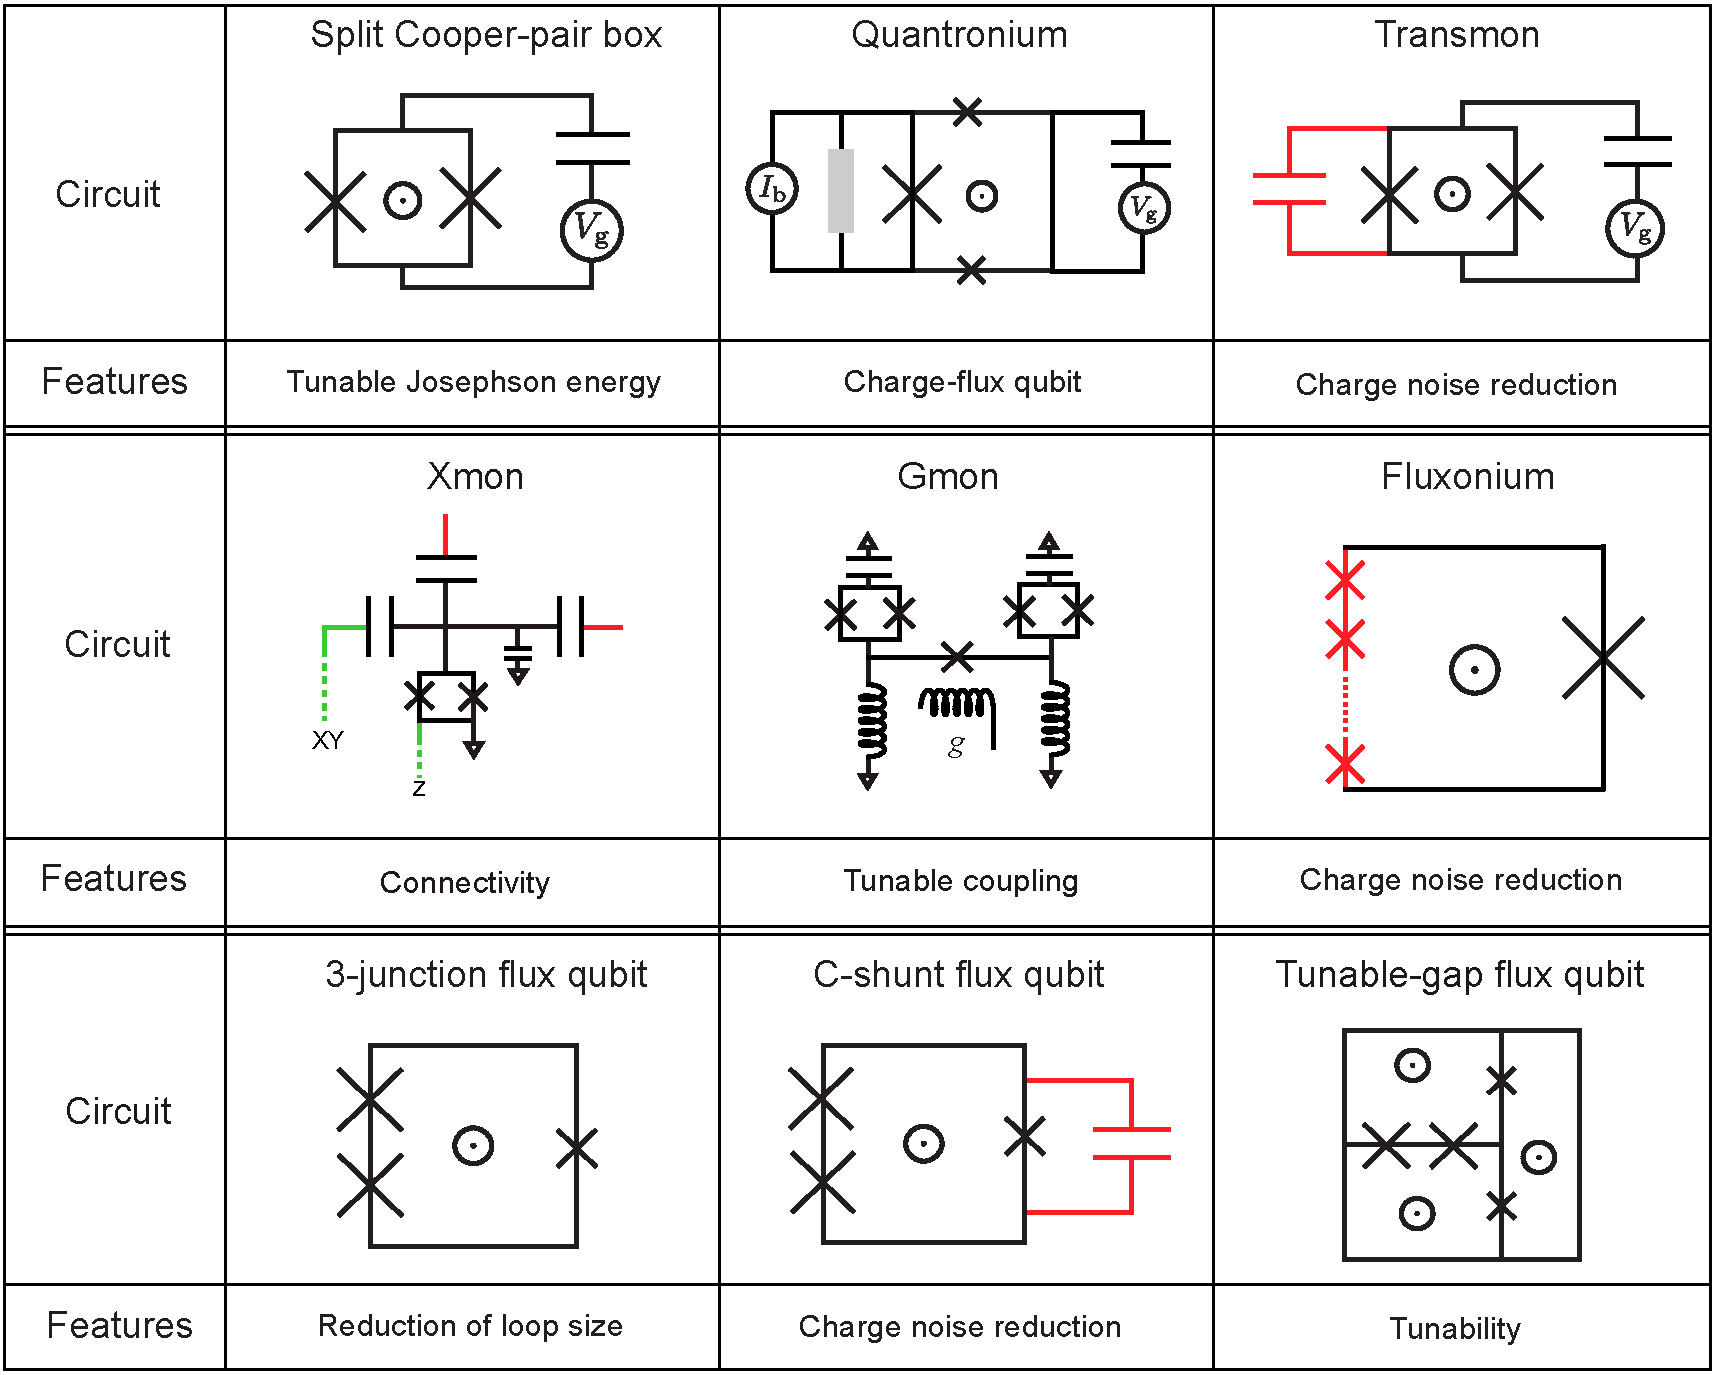
\includegraphics[width=1\linewidth]{Figures/review/QubitExtensions}
   	\caption{超导量子比特的变种,图片来自参考文献\cite{GU20171}。}
   	\label{fig:qubitextensions}
   \end{figure}
   
   跃迁往往是腔和腔之间的一个耦合器控制的,我们可以用一个固定的电容耦合他们,也可以用可控制的耦合器耦合他们。考察两个元件,通常来说他们之间的耦合可以写作:
   \begin{equation}
   	H = H_0 + H_1 + H_{01} = H_0 + H_1 + g(t)\mathcal{O}_0 \mathcal{O}_1
   \end{equation}
   一般来说$\mathcal{O}_i$都是局域在某个元件位置上的算符,因此,当系统足够多,我们可以连接出不一样的空间构型。可以自由的设计耦合常数出现的位置,是超导量子电路这种人工量子材料的优势之一。
   
   此外,上面的哈密顿中,和一般物理学中的最小耦合系数是常数不同,耦合系数是有可能可调的,$g = g(t)$,这种可调的耦合,尤其是动力学过程内可调确保了超导量子电路可以实现各种各样不同的跃迁形式,包括使得光子获得规范势能,以模拟格点规范模型和拓扑绝缘体等等。
   
   除了电路和电路之间的耦合,超导量子电路一般是一个开放体系,还可以和环境产生耦合,从而诞生了环境控制的超导量子电路、人工耗散体系和耗散保护的量子资源等等具有前景的方向。 电路还可以和声波等等模式进行耦合。
   
   这一章节里,第一部分,我们首先参考文献\cite{GU20171}回顾超导量子电路的几大构件,我们着重讨论Transmon Qubit,和量子比特的一种理想电磁环境——3D 腔\cite{reagor2016quantum},以及如何实现超导量子电路之间可以调谐的耦合器。随后在第二部分,利用量子化手续建立超导量子电路的理论模型:我们发现非谐的超导量子电路有典型的原子特征,而腔可以作为原子的辐射场参与“人工原子的偶极相互作用”,我们对超导量子电路建立了量子Rabi模型。我们首先介绍了量子Rabi模型旋波近似的JC模型和它的解析严格解,随后利用算子微扰论当中的resolvent方法讨论Rabi模型的传播子。然后我们讨论超导量子电路上通过一种\textit{in situ}的参变,在旋波近似的条件下演生了一种人工规范场。随后我们介绍三个和关联、几何、对称性有关的应用,一个是超导量子电路如何通过谱测量,精确的确定超导量子电路的能级分布。然后我们介绍超导比特上的几何和乐门的最新进展。
   
   \subsection{超导量子电路的构件\label{sec:fab}}
   	按照前言讨论的,超导量子电路的基础构件就是超导的电容、电感和一些非线性元件。我们首先介绍最重要的非线性元件,约瑟夫森结。约瑟夫森结的研究始于,介观体系是否能表现出来量子特征,介观体系目前看起来显然具备了量子特征。在超导量子电路中,约瑟夫森结的重要意义在于提供了系统很强的非谐性,进而为引进量子计算和定义qubit成为可能。\cite{nakamura1999coherent}
   
   \subsubsection{约瑟夫森结与库伯盒的量子化}
   	约瑟夫森结本身由两个超导的量子结以及一个隔开结的$1-3$nm厚的绝缘层构成,这两个量子结本身构成了一个电容$C_J$。超导Cooper对,可以相干的透过绝缘势垒,从而形成电流。这个电流叫做直流约瑟夫森结电流,$I = I_c \sin \phi$,其中$\phi$是两个超导体之间的相位差,这个相位差和两个结之间的相位差有关$\partial_t \phi = 2eV/\hbar$,$I_c$是和绝缘材料性质有关的特征电流\cite{Makhlin2001quantum}。由上面的两个公式,约瑟夫森结具有能量$E = \int_{-\infty}^{t} V(t')I(t')dt = \frac{\hbar I_c}{2e}(1-\cos \phi) \equiv E_J (1-\cos\phi)$,$E_J$叫做约瑟夫森能量,同时约瑟夫森结也就可以看成一个有效的电感$L = \frac{\hbar}{2eI_c \cos \phi}$。因此我们一般将一个实际的约瑟夫森结化作$E_J$和$C_J$.\cite{you2003quantum}
   	
   	
   
   	为了量子化一个系统,我们需要:(1)体系的广义坐标,(2)拉格朗日量,(3)体系的原始哈密顿量。我们选取超导量子电路的正则坐标为结磁通:
   	\begin{equation}
   	\Phi_n(t) = \int_{-\infty}^t V_n(t')dt'
   	\end{equation}
   	以及结电荷:
   	   	\begin{equation}
   	Q_n(t) = \int_{-\infty}^t I_n(t')dt'
   	\end{equation}
   	其中$I_n$是通过第$n$个节点的结电流。
   	
   	按照基尔霍夫定律,有:
   	\begin{equation}
   	\sum_{\text{a loop}} \Phi_b = \Phi_{\text{ext}}
   	\end{equation}
   	而$\Phi_{\text{ext}}$是外加的磁通,外加磁通需要满足磁通量子化条件$\Phi_{\text{ext}} = n \Phi_0 \equiv n\frac{h}{2e}$.
   	基尔霍夫定律可以作为调节消去自由度,因此不会作为体系的第一类约束进入量子化步骤。
   	
   	有了这些广义坐标,我们就可以写出由这些广义坐标定义的拉格朗日量$\mathcal{L} = \mathcal{L}(\dot{\Phi}_n, \Phi_n)$,进而得到体系的广义动量和拉格朗日量:
   	\begin{equation}
   	\Pi_n = \frac{\partial \mathcal{L}}{\partial \dot{\Phi}_n} \quad H = \sum_n \Pi_n \dot{\Phi}_n - \mathcal{L}
   	\end{equation}
   	
   	如果一个体系的广义动量和广义坐标的导数有关,但是和广义坐标本身无关,我们就可以直接使用泊松括号到量子对易括号的映射来量子化整个系统:
   	\begin{equation}
   	[\Phi_m, \Pi_n] = i\hbar \delta_{mn}
   	\end{equation}
   	
   	如果广义动量和广义坐标有关,那么这个体系将会有第二类约束,定义量子对易括号可能会带来不自恰的结果,这个时候我们应该使用狄拉克广义哈密顿动力学出发,去量子化整个系统。
   	
   	好在我们后面讨论的例子不需要用到复杂的狄拉克量子化步骤。电容内的能量$\frac{CV^2}{2}$对应着系统的动能,而电感对应着系统的势能$\frac{LI^2}{2}$;利用$V = \dot{\Phi}, LI^2/2 = \frac{(LI)^2}{2L} = \frac{(\int dt V(t'))^2}{2L} = \frac{(\Phi - \Phi)^2}{2L}$其中$\Phi = \Phi_1 - \Phi_2$对应端口的电压差的积分。我们接下来讨论一个电容和一个约瑟夫森结、一个电源串联的系统,这个系统一般被称作库珀对盒子:
   	\begin{equation}
   	\mathcal{L} = \frac{C_g (\dot \Phi - V_g)^2}{2} + \frac{C_J \dot \Phi^2}{2} - E_J(1-\cos\frac{2e\Phi}{\hbar})
   	\end{equation}
   	正则变量$\Pi = (C_J + C_g)\dot \Phi - C_gV_g$, 因此$[\Phi, \Pi] = i\hbar$, 定义$E_c = \frac{e^2}{2(C_g + C_J)}$为单电子电能,库伯对的数量定义为$n = -Q/2e$和相位差$\phi = 2e\Phi/\hbar$, 利用$H = \Pi \dot\Phi - \mathcal{L}$:
   	\begin{equation}
   	H = 4E_C(\hat n-n_g)^2 - E_J \cos\phi
   	\end{equation}
   	得到的对易关系为$[\phi,\hat n] = 1$。$\hat n$沿袭了上面库伯对数的定义,但是与$n$区别开来。
   	
   	下面我们去找承载了这个模型的一组希尔伯特空间,最自然的就是:
   	\begin{equation}
   	\hat n \ket{n} = n \ket{n}
   	\end{equation}
   	体系有一个自然的产生湮灭算符$e^{\pm i \phi}$,我们可以如下验证:
   	\begin{equation}
   	\begin{aligned}
   	e^{i\phi} \hat n e^{-i\phi} &= \hat n + [\phi,\hat n] + \frac{1}{2!}[\phi,[\phi,\hat n]] + \cdots = \hat n + 1\\
   	\hat{n}(e^{i\phi}) \ket{n} &=( e^{i\phi}-e^{i\phi} n )\ket{n} = (n-1)e^{i\phi} \ket{n-1}
   	\end{aligned}
   	\end{equation}
   	因此$e^{\pm i\phi} \ket{n} = \ket{n \mp 1}$,进而利用$\cos \phi = \frac{e^{i\phi} + e^{-i\phi}}{2}$得到:
   	\begin{equation}
   	H = \sum_n \{V_n \ket{n} \bra{n}- t (\ket{n+1}\bra{n} + h.c.)   \}
   	\end{equation}
   	其中 $V_n = 4E_C (n-n_g)^2, t = -\frac{E_J}{2}$. 注意$[e^{i\phi}, \hat n] = e^{i \phi}$事实上和辛结构有关。
   	
   	\subsubsection{传输线腔的量子化}
   	超导传输线腔由均匀交叉分布的(自身的)电容和电感构成。按照麦克斯韦方程,超导传输线腔中的流满足波动方程。进而体系具有最大的“速度”尺度$\sim v_m = \frac{1}{\sqrt{L_0 C_0}}$,接下来我们将利用这一点构造Lorentz不变的腔的拉格朗日量,进而类似无质量Klein-Gordan场,我们可以通过规范无关的办法量子化这个体系。注意现在场变量是$\Phi_n(t)\to \Phi(x,t)$依然是“结点”磁通,但现在这个结点磁通还要满足“场方程”,而量子化场方程的方法叫做二次量子化。
   	
   	按照经典无限长谐振腔里的麦克斯韦理论,场变量满足波动方程:
\begin{equation}
\label{eq:wave_TLR}
\frac{\partial^2 \Phi(x,t)}{\partial t^2} - v^2_m \frac{\partial^2 \Phi(x,t)}{\partial t^2} = 0
\end{equation}
很显然这个方程具有洛伦兹不变性,更具对称性和方程的阶数不难猜出拉格朗日密度$L = \int_{-\infty}^{+\infty} dx \mathcal{L}$:
\begin{equation}
\mathcal{L} = \nabla^2 \Phi = g^{i,j} \partial_i \partial_j \Phi(x,t) = \frac{C_0}{2}(\partial_t \Phi(x,t))^2 - \frac{1}{2L_0} (\partial_x \Phi(x,t))^2
\end{equation}
体系的欧拉-拉格朗日方程$\partial_\mu \frac{\partial \mathcal{L}}{\partial(\partial_\mu \Phi)} = \frac{\partial\mathcal{L}}{\partial\Phi}$就恰好能给出Eq.~\ref{eq:wave_TLR}. 我们下一步求出正则变量:
\begin{equation}
\Pi(x,t) = \frac{\partial \mathcal{L}}{\partial_t \Phi} = C_0 \partial_t \Phi \equiv Q(x,t)
\end{equation}
这里$\Pi(x,t) \sim CU$有着电荷的物理意义因而命名为$Q(x,t)$. 采用标准的正则变换得到哈密顿密度$H = \int_{-\infty}^{+\infty} dx \mathcal{H}$:
\begin{equation}
\mathcal{H} = \frac{Q(x,t)^2}{C_0} + \frac{1}{L_0}(\partial_x \Phi(x,t))^2
\end{equation}
施加场的正则对易关系$[\Phi(x),Q(x')] = i\hbar \delta(x-x')$。即得到了场的量子化。

将场是做谐振子模式,我们还有一种定义场的办法:
\begin{equation}
\Phi_\sigma = \sqrt{\bar Z_0 \over{4\pi}} \int_{0}^{\infty} \frac{d\omega}{\sqrt{\omega}}(a_{\omega,\sigma}e^{-i(\sigma kx+\omega t)}+h.c)
\end{equation}
其中 $\sigma = \text{R/L} = \pm 1$, $Z_0 = \frac{L_0}{C_0}$是传输线的特征阻抗, 产生湮灭算符满足:
\begin{equation}
[a_{\omega,\sigma}, a^\dagger_{\omega',\sigma'}] = \delta(\omega' - \omega) \delta_{\sigma \sigma'}
\end{equation}

下面我们将传输线腔施加边界条件使得场在$x = 0. x=d$处等于0: $\Phi(0,t) = \Phi(d,t) = 0$, 这立即给出$a_{\omega, L} = -a_{\omega,R}$, 同时给出来腔的本征模式:
\begin{equation}
\omega_n  = \frac{n \pi v}{d} = \frac{n \pi }{d \sqrt{C_0 L_0}}
\end{equation}
因此腔最后的哈密顿就是$H = \sum_{n} \hbar \omega_n (a^\dagger_{\omega_n} a_{\omega_n}) + \text{vacuum energy}$,我们一般只考虑腔的最低的一个模式,因此腔的哈密顿就是
\begin{equation}
H = \hbar \omega_r (a^\dagger a + \frac{1}{2})
\end{equation}
      \subsubsection{常见的简单量子比特}
      下面我们简单介绍一下几种常见的量子比特\cite{girvin2009circuit,martinis2009superconducting}。
      
      \begin{figure}
      	\centering
      	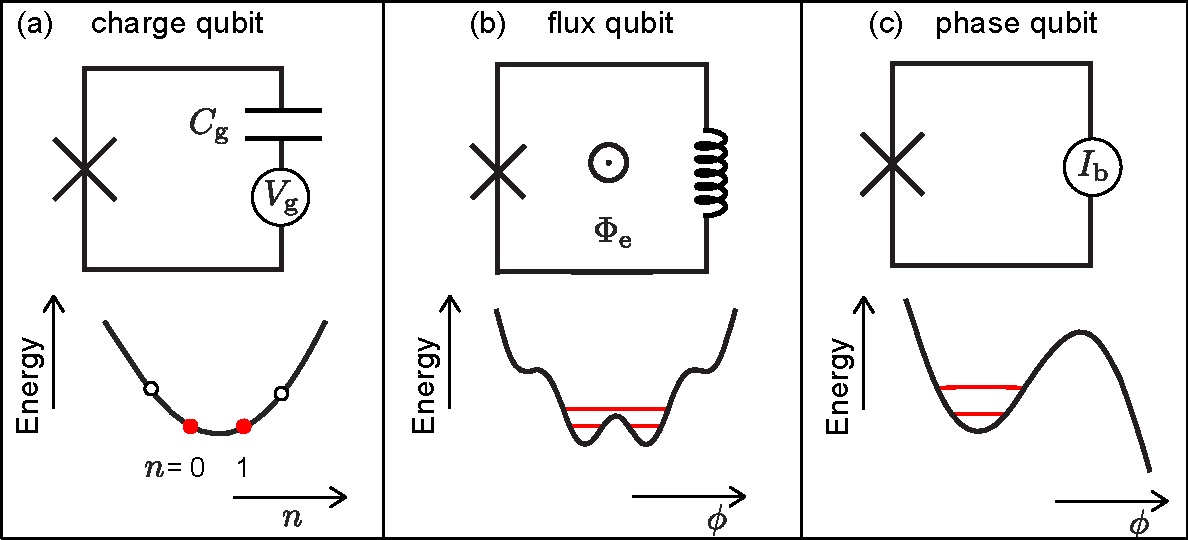
\includegraphics[width=0.9\linewidth]{Figures/review/ThreeQubits}
      	\caption{三种基本的比特构型,图片来自参考文献\cite{GU20171}}
      	\label{fig:threequbits}
      \end{figure}
      
      首先是单结双器件比特。刚刚我们介绍的库珀对盒子,就是Charge量子比特,是由电压源控制的、含有一个约瑟芬森结和一个电容的器件\cite{astafiev2004quantum}。根据我们刚刚的推导,我们得到了: 
      \begin{equation}
      H = \sum_n V_n \ket{n} \bra{n} - t_n (\ket{n+1}\bra{n} + h.c.)
      \end{equation}
      这样的器件一般是电荷主导的,i.e,$E_C \gg E_J \gg k_B T$,经过简单的计算,我们就可以知道体系的$n$的涨落不大,而相位涨落很大。
      
      将这个哈密顿量投影到$\{\ket{0}, \ket{1}\}$的子空间中并定义$\sigma_z = \ket{1}\bra{1} - \ket{0}\bra{0}$, $\sigma_x = \ket{1}\bra{0} + \ket{0}\bra{0}$, 投影的哈密顿可以简单的写作:
      \begin{equation}
      H = -2E_C(1-2n_g)\sigma_z - E_J/2 \sigma_x
      \end{equation}
      我们有时候希望$E_C$是可调节,将约瑟夫森结换作一个SQUID我们就会得到一个\textit{in situ}可调的对角项了. 
      
      我们还可以有几种简单的变种,包括flux量子比特\cite{chiorescu2003coherent},由一个约瑟夫森结和一个电感构成,由一个外界磁场源控制。flux比特顾名思义,有一个持续不断的环电流(因而等效为一个磁通)。
      
      
      最后看到phase量子比特\cite{lucero2012computing},由一个约瑟夫森结和一个偏置电流源构成,这个结一般做的非常大$E_J/E_C \approx 10^6$因此具有偏置电流噪声的不敏感性。但是和charge比特不同的是,由于这种比特的有效势能没有宇称,因此对电磁噪声敏感。
      
      添加不同的电路原件可以组成各种各样非常不同的量子比特结构,他们各自有自己优良的结构特征,也有不足。感兴趣的读者可以参考文献\cite{GU20171}。
	  \subsubsection{量子比特之间的\textit{in situ}耦合器}
	  我们接下来讨论量子比特之间的耦合。最直接的耦合办法是在两个电路的端口上引入一个电容,两个系统(下面考虑两个库珀对盒子)的哈密顿量可以写作
	  \begin{equation}
		\begin{aligned}
			H &= H_0 + H_1 + H_{01}  \\
			  &\equiv E_{C1} (n_{g1} - \hat n_1)^2 - E_{J1}cos\phi_1\\
			  &+ E_{C2} (n_{g2} - \hat n_2)^2 - E_{J2}cos\phi_2\\
			  &+ E_m(n_{g1} -\hat n_1)(n_{g2}-\hat n_2)
		\end{aligned}
	  \end{equation}
	  如果两个体系都只考虑最低的两个能级,系统的耦合就可以写作:
	  \begin{equation}
		  H = \frac{1}{4}(E_{C1} + E_{C2}) + {1 \over 4} E_m \sigma^x_1 \sigma^x_2 - {1\over 2}E_{J1} \sigma^z_1 - {1\over 2}E_{J2} \sigma^z_2 
	  \end{equation}
	  如果两个体系是自由腔或者非线性腔,我们可以得到:
	  \begin{equation}
	  \label{eq:JC}
		H = \omega_1 a_1^\dagger a_1 + \omega_2 a_2^\dagger a_1 + g_{12}(a_1^\dagger a_2 + h.c.) + \text{nonlinear terms}  
	  \end{equation}
	  这样的耦合也可以发生在超导电路和腔之间,这样就诞生了超导量子电路量子电动力学(circuitQED)。叫这个名字的原因是,非线性超导电路本身的能级分布
	  就和自然原子类似,因而是一个"人工原子"。而腔中含有玻色模式,因而是一个微波光场。将这两个系统耦合起来,正是量子光学\cite{scully1999quantum},或腔量子电动力学\cite{walther2006cavity}研究的主题。
	  我们可以在这样的耦合平台上研究各种各样的相互作用,但是我们接下来要介绍一个超导量子电路和自然界中原子-物质相互作用非常大的一点不同,那就是超导量子电路的之间的耦合可以含时可调\cite{niskanen2007quantum,chen2014qubit,blais2003tunable},因而是一个很好的研究各种相互作用导致的新奇物象的人工平台\cite{wallraff2004strong,you2006superconducting}。


	   超导量子电路的意义在于,任何的控制脉冲,例如电压和磁通信号,都是可以在一个范围内固定(直流)甚至是含时间变化的(交流)。我们自然会去思考了,我们有没有可能实现可调节的耦合,特别是可以\textit{in situ} 调节的耦合呢?所谓\textit{in situ}指的是,在ns级别的
	   量子过程中这个耦合可以含时的条件,i.e,我们要实现下面的哈密顿:
	   \begin{equation}
		H = \omega_1 a_1^\dagger a_1 + \omega_2 a_2^\dagger a_1 + g_{12}(t)(a_1^\dagger a_2 + h.c.) + \text{nonlinear terms} 
	   \end{equation}
	   答案是完全可以的。 简单的来说,我们将两个qubit之间的耦合器换成一个耦合回路,再通过一个外加的磁通来调节它,就可以获得这样一个功能的器件了\cite{niskanen2007quantum,chen2014qubit,blais2003tunable}。随后我们会使用这样的技术去展示如何在超导量子电路中实现模拟的规范场,
	   这样的完全含时可控的量子物质,还是一个非常好的演示量子计算和量子控制方法的平台。
   
   \subsection{超导量子电路的理论模型}
   超导量子电路量子电动力学中,最基本的数学模型是Rabi模型\cite{you2006superconducting},经过合理的近似之后我们得到了Jaynes-Cumming 模型(JC模型)。超导量子电路天生是一个光子
   体系\cite{blais2004cavity,blais2004cavity},会和电磁环境耦合产生自然的退相干,也就是有耗散和激励。
   \subsubsection{JC模型和拉比震荡}
   量子光学(cavityQED, circuitQED)中最基本的、有关光和物质相互作用的模型是量子Rabi模型,它的哈密顿量写作:
	   \begin{equation}
		   H_{\text{Rabi}} = \omega_r (a^\dagger a + { 1\over 2}) + \frac{\omega_q}{2} \sigma_z + g(a^\dagger + a)(\sigma_+ + \sigma_-)
	   \end{equation}
	其中, $2g$代表一个实验参数:真空拉比频率。 而$a^\dagger$和$a$代表玻色的产生算符和湮灭算符。 $\sigma_+, \sigma_-$代表$\sigma_z$表象
	下的阶梯算符$\sigma_+ = \ket{e} \bra{g}$, $\sigma_- = \ket{g}\bra{e}$.

	上面定义的哈密顿量在我们的超导量子电路里可以看成一个电路和传输线腔之间的耦合,而在量子光学中可以看成一个原子和F-P腔中的某个驻波模式的耦合。
	因此我下面不加区分的使用原子(超导电路人工原子、量子比特)和腔(光子、传输线腔)。
	   
	分析一下哈密顿量里的每一个项。前两项是原子和腔自己的自由哈密顿量,Rabi模型中,相互作用项有四个$\sigma_+ a, \sigma_- a^\dagger, \sigma_- a, \sigma_+ a\dagger$.
	\begin{enumerate}
		\item $\sigma_+ a$表示湮灭一个光子,原子被激发,可以看成原子吸收了光子。
		\item $\sigma_- a^\dagger$原子的激发被消去,同时激发一个光子,可以看成原子辐射了光子。
		\item $\sigma_- a$原子和光子都被消去。这是真空项。
		\item $\sigma_+ a^\dagger$原子和光子都产生。这是真空项。
	\end{enumerate}
	在近耦合的时候,即$|\omega_q - \omega_r|,g \ll \omega_q + \omega_r$的时候,体系的动力学能标主要由$\omega_q- \omega_r$支配,
	而$\omega_q + \omega_r$是高频项,在动力学能标下平均值几乎为零。因此我们可以设想,体系占主导的项主要由原子和腔的自由能量,以及相互作用能量的前两项。
	丢去后面两项的近似,叫做旋转波近似,得到的模型就是我们要讨论的JC模型\cite{you2011atomic}:
	\begin{equation}
		H_{\text{JC}} = \omega_r (a^\dagger a + \frac{1}{2}) + \frac{\omega_q}{2} \sigma_z + g(a^\dagger \sigma_- + a \sigma_+)
	\end{equation}
	
	如果原子处于激发态,光场初始处于真空态,且光场和原子处于共振的时候,我们可以通过求解薛定谔方程得到体系的运动方程为一个周期的运动。这个真空腔中,激发的原子的不断被激发、不断产生光子的过程叫做真空拉比振荡。然而,腔一般是有耗散的,假设体系处于一个热浴中,我们可以导出所谓的Linblad主方程\cite{gardiner2004quantum}:
	\begin{equation}
	\dot \rho(t) = -i[H(t),\rho(t)] + \mathcal{L}_{C_n}[\rho(t)]
	\end{equation}
	其中$\mathcal{L}_{C_n}[\rho(t)] = \frac{1}{2}[2C_n \rho(t)C_n^\dagger - \rho(t) C_n^\dagger - C_n^\dagger C_n \rho(t)]$, $C_n = \sqrt{\gamma_n} A_n$是系统耗散过程的湮灭算符。
\begin{figure}
	\centering
	\includegraphics[width=0.9\linewidth]{Figures/mine/VacuumRabos}
	\caption{真空拉比振荡,耗散的图即考虑了光子的耗散$A_1 = a$, 也考虑了原子的退相干$A_2 = \sigma_x, A_3 = \sigma_z$。}
	\label{fig:vacuumrabos}
\end{figure}
	
	但是,这种真空拉比振荡并不一定是一个良定义的可观测过程,可观测的量一般都是关联函数,例如发射谱函数:
	\begin{equation}
	S(\omega) = \int_{-\infty}^{+\infty} \avg{a^\dagger(t) a(0)} e^{-i\omega \tau} d\tau
	\end{equation}
	
	\begin{figure}[h]
		\centering
		\includegraphics[width=0.9\linewidth]{Figures/mine/VacuumRabisp}
		\caption{真空拉比劈裂。两个劈裂峰的距离差刚好就是$2g$,因此这个实验可以用来测量光和原子的相互作用强度。}
		\label{fig:vacuumrabisp}
	\end{figure}
对于刚刚的共振真空拉比振荡,我们可以得到它的辐射谱是一个对称的双峰,如图\ref{fig:vacuumrabisp}所示。两个峰的频率劈裂恰好就是$2g$。但是,我们在实验上其实并不知道什么时候光场会和原子共振,一般是用一个机械仪器来调控腔壁的距离来控制光子的频率\cite{puri1987finite}。

因此我们的实验应该是通过不断的扫频得到“反交叉曲线”。在远离共振的时候,光子是光子的激发,而原子几乎很难激发,在近共振的时候能级就会趋向简并而得到一个反交叉。

\begin{figure}
	\centering
	\includegraphics[width=0.9\linewidth]{Figures/mine/VacuumRabsp2.png}
	\caption{真空拉比劈裂在原子和光场之间失谐情况下的“反交叉”情况。注意到大失谐情况下,体系的功率谱几乎是稳定的,这就启发我们建立一个有效模型。}
	\label{fig:vacuumrabsp2}
\end{figure}


通过验证$[H,N] = 0,N = a^\dagger a + \sigma_+ \sigma_-$这个哈密顿具有守恒量$N$. 因此在$N$的本征表象下,哈密顿是块对角的,而$\left \langle \sigma_+ \sigma_- \right\rangle = 0,1$
因此这个子空间的维数是2,让我们选取这个子空间为$\{\ket{g}\ket{n+1}, \ket{e}\ket{n}\}$,在这个子空间中,哈密顿可以被对角化。本征能量为:
\begin{equation}
E_n^\pm = E(\ket{\pm,n}) = \omega_r (n+\frac{1}{2})\pm \frac{1}{2} \sqrt{\Delta^2 +\Omega_{n,r}^2}
\end{equation}
对应的本征态是:
\begin{equation}
\begin{aligned}
\ket{+,n} &= \cos(\frac{\theta_n}{2})\ket{e}\ket{n} + \sin(\frac{\theta_n}{2})\ket{g}\ket{n+1}\\
\ket{-,n} &= -\sin(\frac{\theta_n}{2})\ket{e}\ket{n} + \cos(\frac{\theta_n}{2})\ket{g}\ket{n+1}
\end{aligned}
\end{equation}
其中$\Delta = \omega_q - \omega_r$, $\Omega_n = \sqrt{\Delta^2 + (n+1)\Omega_0^2}$其中$\Omega_0 = 2g$。这也是前文中为何将$2g$叫做真空拉比频率的原因。

\begin{figure}[h]
	\centering
	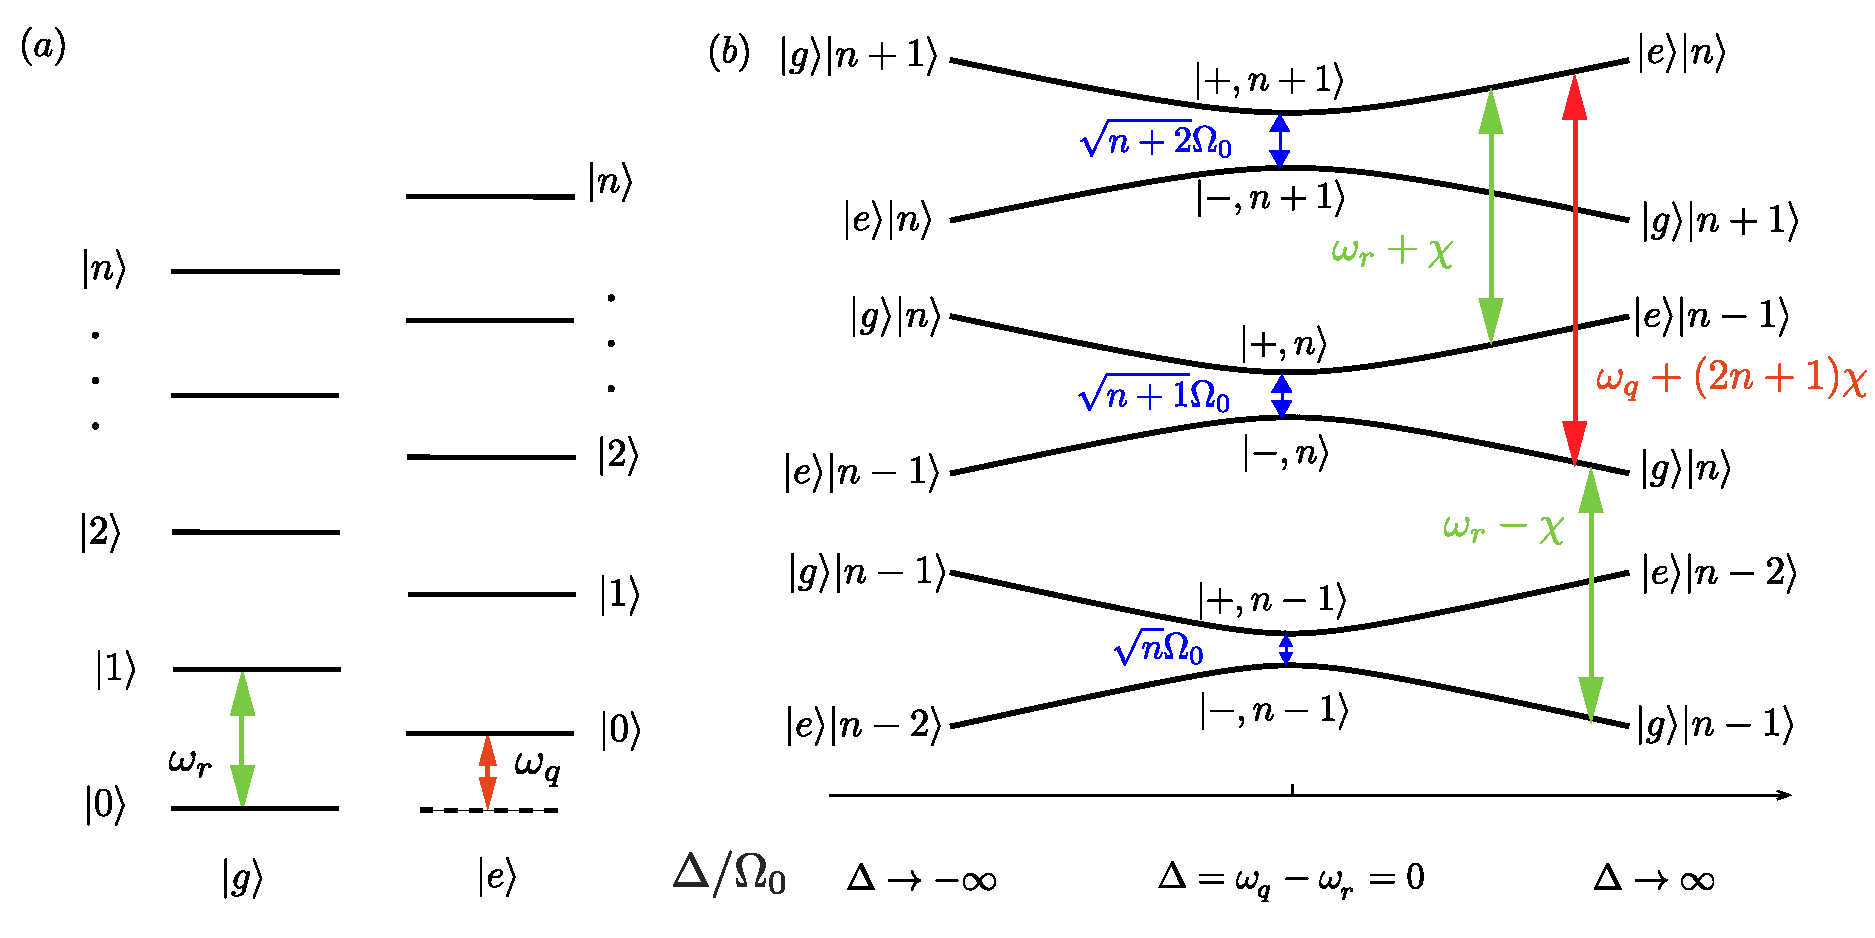
\includegraphics[width=0.9\linewidth]{Figures/review/DressedStates}
	\caption{JC模型的坠饰态。图片来自参考文献\cite{GU20171}。}
	\label{fig:dressedstates}
\end{figure}
这样的本征态又叫做坠饰态,坠饰态下,系统的哈密顿量可以写作:
\begin{equation}
H = -\frac{\Delta}{2}\ket{g,0} \bra{g,0} + \sum_{0}^{\infty} (E^\sigma_n \ket{\sigma,n} \bra{\sigma,n})
\end{equation}

这样的坠饰态,能级之间的非谐是稳定的。因此基于坠饰态也能进行量子计算\cite{timoney2011quantum}。由于坠饰态是原子和光场的一种纠缠特征,所以其上也有非平庸的纠缠\cite{phoenix1991establishment}。

我们再来观察真空拉比劈裂。我们发现体系在大失谐的情况下,体系的功率谱几乎是不变的,那么我们应该发展一套大失谐情况下的有效模型,来标准这一类模型$|\omega_g -\omega_r| = |\Delta| \gg g$利用Schrieffer-Wolff变换$U = \exp [g(a^\dagger \sigma_- - a \sigma_+)/\Delta]$可以得到有效模型:

\begin{equation}
H_{\text{eff}} = [\omega_r + \frac{g^2}{\Delta} \sigma_z] a^\dagger a + \frac{1}{2}(\omega_q + \frac{g^2}{\Delta})\sigma_z
\end{equation}
这样的模型的物理意义是,光子的频率经历了一个$\chi = \frac{g^2}{\Delta}$的平移,或者说,原子的能级差打开了一个$2\chi n$的额外能隙,这个劈裂可以看成一种stack效应。

 \subsubsection{Rabi模型}
 近年来,由于技术和新型量子比特的发展,我们现在可以实现基于超导量子电路平台的超强耦合\cite{wallraff2004strong},因此我们可以继续研究在circuitQED的强耦合模型,即,JC模型适用性不好的区段,例如Rabi模型。
	   
	   \begin{figure}
	   	\centering
	   	\includegraphics[width=0.9\linewidth]{Figures/review/Schuster}
	   	\caption{超导量子电路的相互作用强度可以达到超强耦合,优于其他的平台。图片来自参考文献\cite{GU20171}。}
	   	\label{fig:schuster}
	   \end{figure}
   
	   上面我们已经给出了Rabi模型的哈密顿量:
	   	   \begin{equation}
	   H_{\text{Rabi}} = \omega_r (a^\dagger a + { 1\over 2}) + \frac{\omega_q}{2} \sigma_z + g(a^\dagger + a)(\sigma_+ + \sigma_-)
	   \end{equation}
	   
	   我们现在来分析这个模型。 这个模型具有对称性:$\Pi = -\sigma_z (-1)^{a^\dagger a}$满足$[H,\Pi] = 0$。问题是这个对称性不能给出更多的关于可解性的解答。
	   
	   因此我们不妨使用微扰论即考虑$H_{\text{Rabi}} = H_{\text{JC}} + g( \sigma a+ \sigma_+ a^\dagger)$。为了求解这个模型,我们先写出各个非零的哈密顿: 
	   \begin{equation}
	   \begin{aligned}
	   H_{mg,ng} &={\omega_r n{\delta _{m,n}} + g \sqrt {n + 1} {\delta _{n + 1,m}} +g \sqrt {n - 1} {\delta _{n - 1,m}}}\\ 
	   H_{mg,ne} &= \frac{\omega_q}{2}\\
	   H_{me,ng} &= H_{mg,ne}\\
	   H_{me,ne} &={\omega_r n{\delta _{m,n}} - g \sqrt {n + 1} {\delta _{n + 1,m}} - g \sqrt {n - 1} {\delta _{n - 1,m}}}\\
	   \end{aligned}
	   \end{equation}
	  
我们关心的动力学主要来自传播子:
\begin{equation}
U_{ai, bj} (t)= \bra{a,i } e^{-iH_{\text{Rabi}}t} \ket{b,j}
\end{equation}

\begin{figure}
	\centering
	\includegraphics[width=0.7\linewidth]{Figures/Feynman/FigFourVerticesRabi}
	\caption{Rabi模型传播子的费曼图表示,来自参考文献\cite{di2017feynman}。}
	\label{fig:figfourverticesrabi}
\end{figure}
利用格林函数,容易写出传播子为:
\begin{equation}
U_{ai, bj} (t)= \frac{i}{2\pi} \int dz G_{ai,bj} (z) e^{-izt}
\end{equation}
其中$G_{ai,bj}$是拉比模型的resolvent,定义$H_{\text{JC}}$的resolvent为$G_0 = (z- H_{\text{JC}})^{-1}$以及$H_{\text{Rabi}}$对应的resolvent $G = (z- H_{\text{Rabi}})^{-1}$和微扰相互作用$V = g( \sigma a+ \sigma_+ a^\dagger)$
我们有Dyson方程:
$G = G_0 + G_0 VG_0 + G_0 + G_0 V G_0 + \cdots$
各个矩阵元可以很方便的使用费曼图计算,请参考文献\cite{di2017feynman},我们可以得出
\begin{equation}
\begin{aligned}
{G_{en,en}}\left( z \right) &= \frac{{\left( {z - \left( {n + 1} \right)\omega_r } \right)}}{{\left( {z - \omega_q  - n\omega_r } \right)\left( {z - \left( {n + 1} \right)\omega_r } \right) - \left( {n + 1} \right){g^2}}}\\
{G_{en,g\left( {n + 1} \right)}}\left( z \right) &= \frac{{\sqrt {n + 1} g}}{{\left( {z - \omega_q  - n\omega_r } \right)\left( {z - \left( {n + 1} \right)\omega_r } \right) - \left( {n + 1} \right){g^2}}}\\
{G_{gn + 1,gn + 1}}\left( z \right) &= \frac{{z - \omega_q - n\omega_r }}{{\left( {z - \omega_q  - n\omega_r } \right)\left( {z - \left( {n + 1} \right)\omega_r } \right) - \left( {n + 1} \right){g^2}}}
\end{aligned}
\end{equation}

\begin{figure}
	\centering
	\includegraphics[width=0.7\linewidth]{Figures/Feynman/FigFeynmanFirst3Diagrams}
	\caption{一个算符的级数展开的费曼图表示,来自参考文献\cite{di2017feynman}。}
	\label{fig:figfeynmanfirst3diagrams}
\end{figure}

现在也有利用坐标表象证明了Rabi模型的完全可解性的研究,但是是利用特殊函数的性质,事实上,利用resolvent和泛函分析的知识,到这一步我们已经可以看出来Rabi模型至少是近可积模型。利用resolvent我们不仅仅可以计算传播子,通过分析Resolvent的奇点,我们还可以求解体系能谱对Rabi模型的修正。

值得一提的是,Rabi模型看起来是一个单体模型,不存在多体中的温度相变。但是,在相变的扩展意义,量子相变下,即量子涨落和量子相互作用带来的相变的时候,我们发现在大失谐情况下的Rabi模型是有非平庸的量子相变的。这个相变可以从朗道对称性破缺理论解释。我们刚刚看到,$[H,\Pi] = 0$体系具有宇称对称性,而小相互作用极限下,基态应当和JC模型一样,因此是$\ket{g,0}$, 而第一激发态要么是$\ket{g,1}$要么是$\ket{e,1}$和基态显然不简并。这就说明小相互作用下,体系发生了对称性破缺——基态不具有这个对称性。满足宇称的子空间应该有两个简并的态,随着相互作用强度的加大,第一激发态和基态的确能简并。

我们首先先从数值上论证系统的相变。图\ref{fig:Rabi}告诉我们,在大失谐情况下,系统$g<g_c$是处于有能隙的对称性破状态状态;而$g>g_c$时,体系的基态发生二重简并,因此回复了对称性。

\begin{figure}
	\centering
	\includegraphics[width=0.9\linewidth]{Figures/Rabi/S4}
	\caption{在大失谐极限$\eta \to \infty$下Rabi模型中的普通相到超流相的相变。(a)体系的基态能量和基态能量的二阶导数。我们可以看出基态能量的二阶导数不是连续的。(b)我们计算第一激发态和基态的能量差,我们容易计算得出,在$g>g_c$之后,基态成为了二重简并的,基态满足了宇称的子空间,因此实际上是$g<g_c$时,体系发生了自发对称性破缺。(c) 随着$\eta \to \infty$体系的相变行为越来越容易体现出来。(d)从Rabi模型到Dicke模型,体系满足同一个标度行为。}
	\label{fig:Rabi}
\end{figure}

近年来,还有研究指出这样的大失谐极限下的Rabi模型的相变可以作为Dicke模型的极限,给出相同的普适类\cite{sun2018out}。

在数值上证明了我们的体系的确会发生相变,我们接下来基于平均场理论来计算一下体系的相变点。

我们利用单个qubit等价于两个费米子场$u,v$的单激发子空间$u^\dagger u + v^\dagger v= 1$首先构造如下的有效作用量:
\begin{equation}
\mathcal{Z} = \int \mathcal{D}(\bar\alpha,\alpha, \bar f,f)e^{-S_0[\bar\alpha,\alpha,\bar f,f]-S_{\text{int}}[\bar\alpha,\alpha,\bar f,f]}
\end{equation}
其中:
\begin{equation}
\begin{aligned}
S_0[\bar \alpha,\alpha] &=\int d \tau \bar \alpha(\partial_\tau + \omega_0) \alpha \\
S_0[\bar f,f] &= \int d \tau \bar f(\sigma_0 \partial_\tau + \sigma_3\frac{\Omega}{2})f\\
S_{\text{int}} &= -\int d \tau \bar f [g(\bar{\alpha}+\alpha)\sigma_1]f\\
\end{aligned}
\end{equation}
注意到体系的约束,我们利用$\delta$函数表出,得到:
\begin{equation}
\begin{aligned}
\mathcal{Z} \to \mathcal{Z} &= \int \mathcal{D}(\bar \alpha,\alpha, \bar f, f) \delta(\bar{f}f-1)e^{...}\\
& =  \int \mathcal{D}(\bar \alpha,\alpha, \bar f, f, \sigma) e^{-\int d\tau \sigma(\tau) (\bar{f}f-1)} e^{...}
\end{aligned}
\end{equation}
考虑傅里叶变换,频率$\omega_n = \frac{2n\pi}{\beta}$,
\begin{equation}
\alpha = \frac{1}{\sqrt{\beta}} \Sigma_{\omega_n} \alpha_n e^{-i \omega_n \tau},
\alpha_n = \frac{1}{\sqrt{\beta}} \int_{0}^{\beta} d\tau \alpha e^{i\omega_n \tau}
\end{equation}
其他的场变量也这样去构造,因此我们可以得到:
\begin{equation}
\begin{aligned}
S &= \sum_{n} \bar{\alpha}_n(-i \omega_n + \omega_0) \alpha_n + \int d \tau \sigma \\
& + \sum_{n} \bar{f}_n [(-i \tilde \omega_n - \sigma)\sigma_0 + \frac{\Omega}{2} \sigma_3] f_n \\
& + \frac{g}{\sqrt{\beta}}\sum_{m,n} \bar{f}_m (\alpha_{m-n} + \bar \alpha_{n-m})\sigma_1 f_n
\end{aligned}
\end{equation}

然后我们将费米场积分掉,得到:
\begin{equation}
S_{\text{eff}} = \int d\tau \bar \alpha (\partial_\tau+\omega_0) \alpha + \sigma  - \text{trln} (-G^{-1})
\end{equation}
其中格林函数 $G^{-1} = \sigma_0 (\partial_\tau-\sigma) + \sigma_3 \frac{\Omega }{2} - g (\bar \alpha + \alpha) \sigma_1$。


在频率空间,我们有:
\begin{equation}
G^{-1}_{m,n} = \delta_{mn} \left( (-i \bar \omega_n-\sigma) \sigma_0 + \frac{\Omega}{2} \sigma_3 \right) + \frac{g}{\sqrt{\beta}} (\alpha_{m-n} + \bar \alpha_{n-m}) \sigma_1
\end{equation}
有了这个作用量,我们想使用平均场理论来描述玻色子的有效哈密顿量。
利用公式 $\delta/\delta X \text{trln} (G^{-1}) = \text{tr} (G\delta/\delta X G^{-1}) = \sum_{m,n} Tr[G_{n,m} \delta/\delta X G^{-1}_{m,n}]$ 其中$Tr$ 是指在局域的希尔伯特空间求迹运算。

我们基于此可以得到:
\begin{equation}
\begin{aligned}
\frac{\delta S}{\delta \alpha_k} &= (-i \omega_k + \omega_0) \bar \alpha_k + \frac{g}{\sqrt{\beta}} \Sigma_{m,n} Tr[G_{n,m} \delta_{(n,{m+k})} \sigma_1] =0\\
\frac{\delta S}{\delta \bar \alpha_k} &= (-i \omega_k + \omega_0) \alpha_k + \frac{g}{\sqrt{\beta}} \Sigma_{m,n} Tr[G_{n,m} \delta_{(n,{m-k})} \sigma_1]=0\\
\frac{\delta S}{\delta \sigma} &= \beta - \Sigma_{m,n} Tr[{G_{n,m} \delta_{mn} \sigma_0}]=0
\end{aligned}
\end{equation}

在平均场尺度,我们猜测 $\left\langle \alpha \right\rangle = \left\langle \bar\alpha \right\rangle = c$ 其中$c^2$ 是系统的总光子数。 因此我们有 $\alpha_n = \sqrt{\beta} c \delta_{n,0}$ (在平均场下),当然 $\bar \alpha_n$也是一样.

因此,在平均场下,系统的格林函数是对角的:
\begin{equation}
\begin{aligned}
\tilde G^{-1}_{mn} &= \delta_{mn} \tilde{G}_{nn}\\
\tilde{G}^{-1}_{nn} &= \left(\begin{array}{cc}
-i \bar \omega_n - \sigma + \frac{\Omega}{2} & 2g c \\ 
2g c & -i \bar \omega_n - \sigma - \frac{\Omega}{2}
\end{array} \right)
\end{aligned}
\end{equation}


注意到$c = 0$ 是前两个方程的一个解。
最后一个方程可以这么来解:
\begin{equation}
\sum_n \frac{1}{i \omega_n - \eta} \simeq \sum_n \frac{1}{i \omega_n e^{-i\omega_n\delta} - \eta} = \frac{\beta}{\exp(\eta)+1}
\end{equation}
这意味着:
\begin{equation}
\beta = \frac{\beta}{\exp(\sigma - \frac{\Omega}{2} ) + 1} +  \frac{\beta}{\exp(\sigma + \frac{\Omega}{2} ) + 1} - \frac{1}{-i \frac{\pi}{\beta} - \sigma + \frac{\Omega}{2}} - - \frac{1}{-i \frac{\pi}{\beta} - \sigma - \frac{\Omega}{2}}
\end{equation}
因此,体系有一个非平庸的自恰场方程的解$\Omega \to \infty$,同时对应了不同的光子数,系统平均场尺度是在$\Omega \to \infty$ 下定义的。 

令$\Omega \to \infty$ 我们找体系的另一个非平庸解$c \ne 0$这可以给出:

\begin{equation}
	\omega_0 c = \frac{2g^2}{\sqrt{\frac{\Omega^2}{4} + 4g^2 c^*c}} \tanh[\frac{c\beta}{2}\sqrt{\frac{\Omega^2}{4}}+4g^2 c^*c]
\end{equation}
$c \ne 0$进而给出$\pm c$满足的方程:
\begin{equation}
\frac{\omega_0 \sqrt{\Omega^2 + 16g^2 c^*c}}{4g^2} = \tanh(\sqrt{\Omega^2 + 16g^2 c^*c} \beta /4) 
\end{equation}
经过复杂的计算我们发现这个相的稳定条件就是$\frac{\delta^2 S_{\text{eff}}}{\delta c^2} >0 \to g >0, \Omega \to \infty$。因此系统在大失谐的情况下的确有一个相变点$g_c = \sqrt{\omega_0 \Omega}/{2}$。有兴趣的读者可以进一步参阅参考文献\cite{sun2018out}。


	\subsubsection{量子控制}
	我们在这里简单的介绍一下量子控制(Quantum control),量子控制指的是通过一些可以人工控制的外加可调脉冲来合成出我们想要的量子操作,是DQS的关键步骤之一。由于我们往往希望这样的量子操作,i.e,量子门,具有最优的保真度,因此量子控制一般的任务都叫做量子最优控制。
	\begin{figure}
		\centering
		\includegraphics[width=1\linewidth]{Figures/control/SuppDevice-v0-LR}
		\caption{John Martinis组的可调耦合的超导量子电路。(a)电路的构型。(b)耦合强度可以被磁通调节。来自参考文献\cite{Roushan2017a}。}
		\label{fig:suppdevice-v0-lr}
	\end{figure}
	本节和后面我们会接触到UCSB-Google John Martinis 组\cite{Roushan2017a}里常用的\textbf{可调耦合的超导量子电路}\ref{fig:suppdevice-v0-lr},按照\ref{sec:fab}节的精神,我们有如下的哈密顿量:
	\begin{equation}
	\begin{aligned}
	 {H_{\text{static}}} &= \sum\limits_{j = 1}^2 {{\omega _j}\left( {a_j^\dag {a_j} + \frac{{{\alpha _j}}}{2}a_j^\dag a_j^\dag {a_j}{a_j}} \right)} \\
	  {H_{\text{couple}}}\left( t \right)&= {g_{12}}\left( t \right)\left( {a_1^\dag {a_2} + h.c.} \right)\\
	   {H_{\text{microwave}}}\left( t \right) &= \sum\limits_j {\left( {{\Omega _j}\left( t \right)a_j^\dag + \Omega _j^*\left( t \right){a_j}} \right)} 
	\end{aligned}
	\end{equation}
上面的哈密顿量第三项可以人工控制,它们可以在纳秒尺度人工的调节(实验上很多使用任意波发生器实现),我们有时也叫这样的人工控制为\textit{in situ}的调节,指的是我们可以“在过程中”控制体系的哈密顿量。这些可以控制的量在物理上是这样的:首先两个qubit内部的等效约瑟夫森结能量可以通过通磁通调节,进而$\omega_{1,2}$可以在$6$GHz左右调节,而$g_{12} = g_{12}(t)$和$\Omega_j(t)$可以在ns尺度调节。


现在,静态哈密顿量,也就是第一项,就给出了静态的能谱。选择$\text{span}\{\ket{g,g}, \ket{g,e} \ket{e,g} \ket{e,e}\}$为我们的目标空间,而系统在相互作用表象下的演化为$\tilde U\left( {t,{t_0}} \right) = {\cal T}\exp \left[ { - i\int {\left( {{H_{\text{couple}}} + {H_{\text{Mircowave}}}} \right)dt} } \right]$,至此我们可以阐述量子控制的定义了。量子控制就是去通过含时调节可变的参数,来“构造”我们需要的演化算符,来达到最优的控制效果,获得想要的量子门操作。这就如同我们想要一个飞机从武汉飞往纽约——我们需要去调整飞机发动机的推动,机翼的形状(转弯)等——但现在我们是想实现量子门。
所谓的Optimal Control,就是去选取最优化的 $g\left( t \right),\Omega \left( t \right)$ 去构造出量子计算需要的单比特门和多比特门。

量子控制往往还需要一个优化目标,在超导量子电路中,保真度,或者脉冲定义的门和我们想要的门的接近程度,使我们的优化对象。基于这一点,我们可以利用梯度下降\cite{khaneja2005optimal,floether2012robust}来构造脉冲,这就是GRAPE算法,即Gradient Ascent Pulse Engineering。

	这个最优化问题的解应该是目标希尔伯特空间维数的多项式函数,因为可想而知,脉冲这一个经典信号的信息量相比演化是较少的\cite{lloyd2014information}。因此出于系统对称性的考虑,我们可以使用一些特殊的基函数去叠加出我们的想要的脉冲,这就是参考文献\cite{doria2011optimal,caneva2011chopped}中讨论的CRAB(Chopped Random Basis)算法的基础.
	
	一个关于量子控制的发展很好的综述是\cite{glaser2015training}. 具体在超导量子电路中的实现,在参考文献\cite{egger2014adaptive,egger2013optimized}中有所叙述。
	
	
	量子控制在初期的实验获得了极大的成功。但是,量子控制存在以下几点弊端和缺陷:
	\begin{itemize}
		\item 第一点是很多量子控制的算法不能够确保收敛性;计算起来非常的复杂。
		\item 第二点是对于复杂的门操作,个人计算机难以有效模拟出,但是好在我们知道,对于一个确定体系,确定的门只需要计算一次,而且正如上面所说的,这个计算的复杂度仅仅是目标希尔伯特空间维数的多项式级别的,所以这个弊端还算能够接受。
		\item 给出来的脉冲极其复杂。有的时候,GRAPE和CRAP给出的脉冲抖动非常剧烈,实验难以实现。
		\item 给出来的脉冲可能是对所有的噪声敏感的,那么体系的环境如果在波动,体系的耗散参数发生改变,那么就会要重新跑一遍量子控制算法。
		\item 上面两点的综合就是,任何脉冲上的缺陷都会直接反应到门的保真度上;因此这样的算法实验做起来并不简单。
	\end{itemize}


之后在\ref{sec:holo}小结我们会介绍一些利用物理图像来进行量子控制的例子,例如超导量子电路上的几何和乐门\cite{hong2018implementing,egger2019entanglement}。利用和乐操作,我们不仅仅能够实现非常高的保真度,而且脉冲非常的简单。
   
   
   \subsection{超导量子电路上的人工规范场}
   这一节我们转向讨论在超导量子电路上对光子进行操控,我们考虑一个更加小的主题,那就是如何让超导腔中的光子感受到一个有效的规范势能,这样创造的有效规范势,可以成为我们后面讨论量子模拟格点规范理论和拓扑绝缘体提供非常好的基础。
   
   我们先来阐述一下,考虑一个多腔耦合的JC模型,它的哈密顿写作:
   \begin{equation}
   H = \sum_{i} \omega_i a_i^\dagger a_i  +( \sum_{ij} t_{ij} a_i^\dagger a_j + h.c)
   \end{equation}
   这个模型描述的是有多个耦合谐振腔,光子可以在里面遂穿,是式 \ref{eq:JC}的多格点扩展。其中,$w_i$可以看做体系的on-site 势能,而$t_i$可以看成体系的动能,或者看成光子从一个腔跳到另一个腔的振幅。
   
   所谓的创造人工规范场,也就是$H_{\text{free}} = \frac{\hat p^2}{2m} \to H_{\text{gauge}} = \frac{(\hat p + eA)^2}{2m}$,经过二次量子化和离散化,我们不难得到:$t \to te^{i \phi}$, 其中$\phi = \int_{r_i}{r_j} A(r') dr'$,这个从无规范场替换至有规范场的办法,叫做皮尔斯替换,上面这样的皮尔斯替换针对的是阿贝尔规范场,因为$[e^{i\phi_m},e^{i\phi_n}] = 0$。如果一个腔里面考虑$n$个模式,那么定义$\psi_r = (a_{1,r},a_{2,r},...,a_{n,r})$,格点之间的跃迁现在是一个矩阵$H_{\text{T}} = \sum_r \psi_{r + \delta r}^\dagger T_{r,\delta r} \psi_r$其中$T$是一个$n \times n$的矩阵,这样,我们就可以实现非阿贝尔规范场了。
   
   如何实现这样的有效规范场呢? 我们不妨来看一下,在其他的物理体系中是如何实现的,例如光子学体系和声子学体系。
\subsubsection{其他体系中的人工规范场}
一种超导量子电路的宏观腔阵列,铝制的3D腔\cite{Sirois2015},在室温不超导就可以实现腔内光场的有效规范场\cite{owens2018quarter,anderson2016engineering}。腔的示意图如图. \ref{fig:microwavelatticepic}所示,考虑基本的腔(C1)的一个模式$H_0 = \omega_0 a^\dagger a$,以及另一种腔(C2),每个腔内具有两个$w_0$的光学模式,它的单腔哈密顿量写作$H_1  = \omega_0 (a^\dagger_1 a_1 + a^\dagger_2 a_2)$。在这个腔内放入了YIG小球,因此引入了电磁场和YIG内自旋波模式的耦合,记自旋波模式为$a_{\text{F}}$, 在基$\psi = (a_1,a_2,a_{\text{F}})$下, $H = \psi^\dagger H_{\text{F}} \psi$,其中:
\begin{equation}
H_{\text{F}} = \left(\begin{array}{ccc}
\omega_0 &  & g/\sqrt{2} \\ 
& \omega_0 & ig/\sqrt{2} \\ 
g/\sqrt{2} & -ig/\sqrt{2} & \omega_{\text{F}}
\end{array} \right)
\end{equation}
我们考虑$g\gg \delta E$其中$\delta E$是我们考虑的能标。从C1腔散射进入另一个$C1$腔的低能过程可以利用输入输出理论有效的计算\cite{anderson2016engineering},见,结果是体系获得了一个有效的相位$\phi = \arg(S_{\text{output}} - S_{\text{input}}) \approx \frac{3}{2} \pi$,进而体系的跃迁矩阵实现了$q = 4, p =3$(进而$\phi = \frac{p}{q} 2\pi = \frac{3}{2} \pi$)的Hofstadter模型\cite{anderson2016engineering}。 基于这样的3D腔的实验实现,我们还提出了在超导状态下,利用SQUID参变耦合两个不同的腔,来探究非贝尔的人工规范场\cite{cai2018non}。


%\begin{figure}
%	\centering
%	\includegraphics[width=0.9\linewidth]{Figures/topphoto/MicrowaveLatticePic}
%	\caption{3D腔体系中实现的人工规范场。利用光和YIG的响应会带来一个有效的跃迁相位,可以获得有效的规范场。(a)体系的示意图,相当于一个$q = 4$的Hofstadter模型。 (b)实验装置图,由于是微波波段的实验,腔体的长度接近厘米量级。 (d)通过输入输出实验测得的能带图,以及和Hofstadter模型的对比。图片来自参考文献\cite{owens2018quarter}。}
%	\label{fig:microwavelatticepic}
%\end{figure}

\begin{figure}
	\centering
	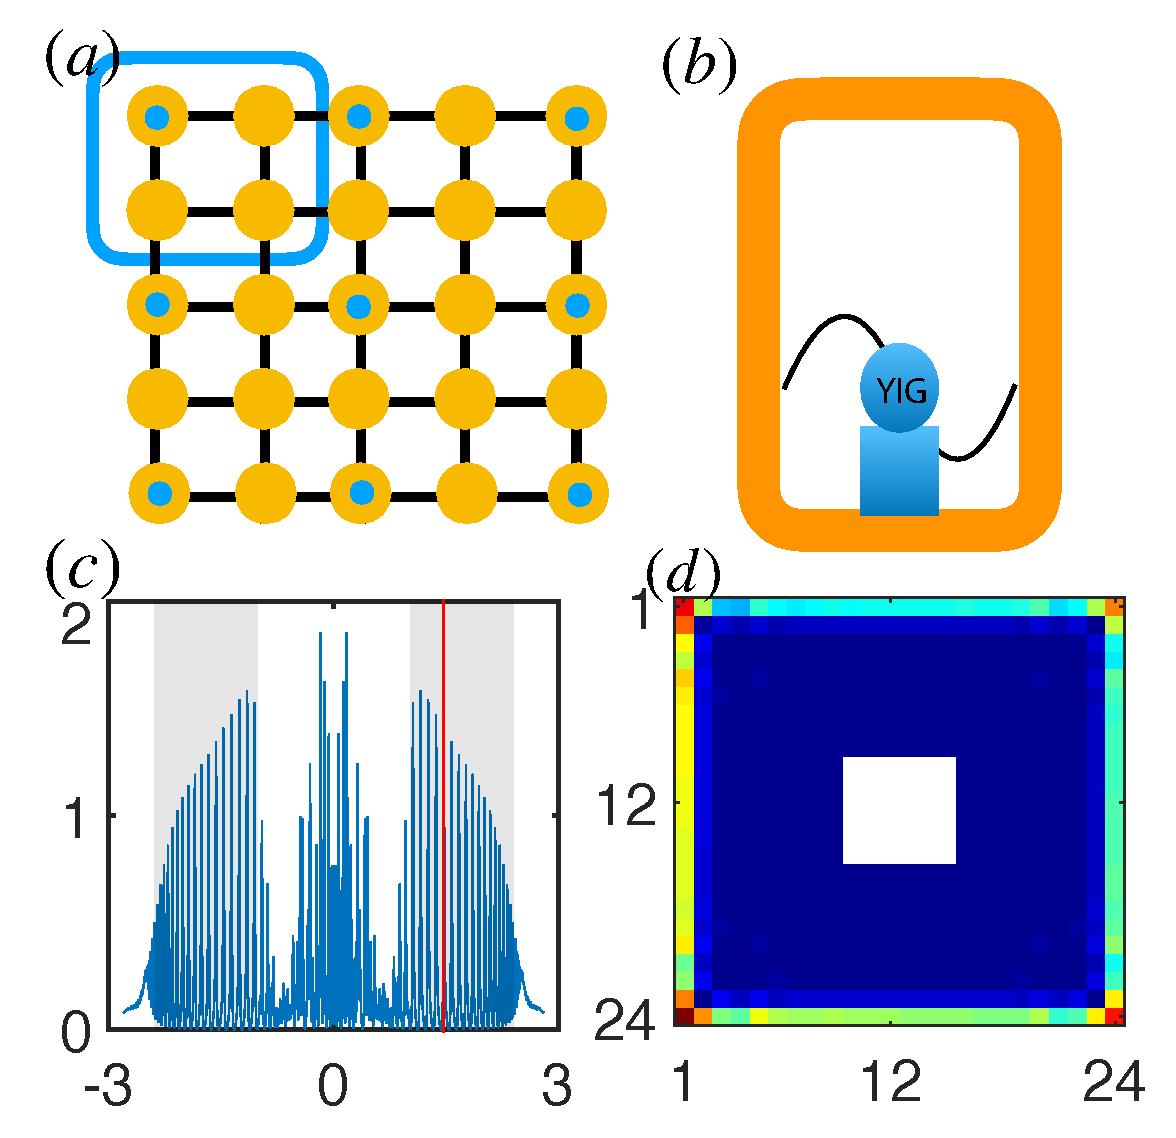
\includegraphics[width=0.9\linewidth]{Figures/topphoto/MicrowaveLatticePicNEW}
	\caption{3D腔体系中实现的人工规范场。利用光和YIG的响应会带来一个有效的跃迁相位,可以获得有效的规范场。\cite{owens2018quarter}(a)体系的示意图,相当于一个$q = 4$的Hofstadter模型。 (b)一个3D腔中放置YIG的实验装置图,由于是微波波段的实验,腔体的长度接近厘米量级。 (c)通过输入输出实验测得的态分布图,以及(d)体系的边缘模式。}
	\label{fig:microwavelatticepic}
\end{figure}


波导阵列的旁轴方程和薛定谔方程具有完全一样的数学形式,在其上实现人工规范场也是有意义的。如图.\ref{fig:mikael-fig1}所示,我们可以写出体系的旁轴方程\cite{rechtsman2013strain,rechtsman2013photonic,rechtsman2013topological}:
\begin{equation}
	i \partial_z E = - \frac{1}{2m} \nabla^2_{x,y} E - V(x,y) E
\end{equation}
其中$m = k_0 $是基础波模波矢,$V(x,y)$是和体系折射率和波矢有关的,可以看做体系的势能,$z$可以看做量子力学的$t$。 利用$x-y$模式分解,不难得到各个格点上局域的波模的分布方程具有如下的形式\cite{rechtsman2013strain,rechtsman2013photonic,rechtsman2013topological}:
\begin{equation}
i \partial_z a_m = - \sum_{\avg{m,n}} t_{m,n} a_n
\end{equation}
对应的哈密顿量是一个二次形$H = \sum_{m,n} \psi^\dagger T \psi$, $\psi = (\alpha_1, \alpha_2,\cdots, \alpha_M)^T$。

产生规范势的办法如图. \ref{fig:mikael-fig1}(c)所示,考虑一个旋转的光纤,顺着光纤建立坐标系,就有$x \to x+ R\cos(\Omega z), y \to y+ R\sin(\Omega z), z \to z$,计算新坐标的度规$g_{i,j}$,发现$\Delta = \nabla^2 \to \Delta$是不变的,而
\begin{equation}
\partial_z \to \partial_z + \hat{\partial}\times \hat \omega = \partial_z + R\Omega(-\sin(\Omega z) \partial_{x} + \cos(\Omega z) \partial_{y})
\end{equation}
新坐标下的方程就是:
\begin{equation}
	i\partial_z E = - \frac{1}{2m} (\partial_{x,y} + iA(z))^2 E - (\frac{mR^2\Omega^2}{2} + V(x,y) )E
\end{equation}
利用模式分解,现在的紧束缚模型成为了:
\begin{equation}
i \partial_z a_m = =\sum_{\avg{m,n}} t_{m,n} e^{i A \cdot (r_m - r_n)} a_n
\end{equation}
正是皮尔斯替换之后的哈密顿量$t \to te^{i \phi}$。

%\begin{figure}
%	\centering
%	\includegraphics[width=0.7\linewidth]{Figures/mikael-fig1}
%	\caption{(a)笔直的波导构成的蜂窝格子,理想图。波导之间的耦合是通过紧邻倏逝波耦合的,因此是一个自然的紧束缚模型。(b)波导阵列的显微成像。实际上,波导阵列可以有非常好的可集成性以及非常低的制造合成误差。(c)旋转波导对应的示意图,这可以创造一个有效的磁场。这样的扭曲光纤可以创造有效的规范势能。图片取自参考文献\cite{rechtsman2013strain,rechtsman2013photonic,rechtsman2013topological}。}
%	\label{fig:mikael-fig1}
%\end{figure}
\begin{figure}
	\centering
	\includegraphics[width=0.7\linewidth]{Figures/topphoto/mikael-fig1}
	\caption{(a)笔直的波导构成的蜂窝格子,理想图。波导之间的耦合是通过紧邻倏逝波耦合的,因此是一个自然的紧束缚模型。(b)波导阵列的显微成像。实际上,波导阵列可以有非常好的可集成性以及非常低的制造合成误差。(c)旋转波导对应的示意图,这可以创造一个有效的磁场。这样的扭曲光纤可以创造有效的规范势能。图片取自参考文献\cite{rechtsman2013strain,rechtsman2013photonic,rechtsman2013topological}。}
	\label{fig:mikael-fig1}
\end{figure}
\begin{figure}
	\centering
	\includegraphics[width=0.9\linewidth]{Figures/topphoto/MH_lattice}
	\caption{纳米光腔中,通过耦合器对应不同模式的光程差不同而创造的有效的自旋轨道耦合。(a)装置的示意图。两个腔(site resonator)中的模式由一个耦合器(link resonator)耦合起来,由于不同的模式经过耦合器的光程不同,因此对应了一个有效的规范势,这可以用输入输出关系理解。(b)装置的有效模型对应,即实现了不同分量的光子(正转反转)感到不一样的规范场,从而实现了量子自旋霍尔效应。(c)装置扩展到二维格点。图片来自参考文献\cite{hafezi2011robust}。}
	\label{fig:mhlattice}
\end{figure}
另一种创造规范势的办法,是通过观察$\psi(r_m) \to e^{i A\cdot (r_m)} \psi(r_m)$就能实现皮尔斯替换,而
$\psi \sim e^{iS}$, $S$是体系的作用量,因此如上替换需要各个格点的作用量改变一个长度且各个格点改变的不一样。
这个思路就诞生了下面的办法,如图\ref{fig:mhlattice}, \ref{fig:mhimaging},\ref{fig:mhinvariants}。

我们可以分析耦合器的输入输出关系来分析这个问题。考虑两个格点和一个耦合器,和其上的某个模式。通过调节耦合器的长度,我们可以让耦合器上的模式和腔里的模式恰好相干相消,相消时候,模式就会局域在腔内。耦合器的输入输出关系给出:$E_n^{\text{out}} = E_n^{\text{in}} + \sqrt{2t} a$, $E$是耦合器上的电场模式,而$a$是腔内的场算符。正如刚刚推倒的,由于光子自由传输,电场之间的关系就是光程差决定的:
$E_{n+1}^\text{in} = -i E^{\text{out}_x \exp(-2\pi i \alpha)}$其中$\alpha$是和系统的折射率、和长度有关的参数,在腔内的场方程$\partial_t a_n = - t a_n - \sqrt{2t} E_n^{\text{in}}$中消去$E$我们得到:
\begin{equation}
	H_{\text{two sides}} = -t a^\dagger_{n+1} a_n \exp(-2\pi i \alpha) + h.c.
\end{equation}
这样就实现了光子的有效规范势。
\begin{figure}
	\centering
	\includegraphics[width=0.8\linewidth]{Figures/topphoto/MH_imaging}
	\caption{(a)装置的示意图。(b)实验结果和理论结果的对比。可见由于体系承载了边缘模式。(c)光子的边缘激发可以绕过一个缺陷继续传播,缺陷的连接方式如图(d)所示。(d)样品的照相图,子图是添加的缺陷。图片来自参考文献\cite{hafezi2013imaging}。}
	\label{fig:mhimaging}
\end{figure}

上面的办法有一些问题。那就是无论是波导还是腔,刻好了之后 ,规范场就难以调节。也有实验实现了可调节的规范势,例如图.\ref{fig:mhinvariants}中的实验。我们能不能通过控制一些脉冲来控制光子感受到的有效规范势能呢?答案是,在超导量子电路中使用参变耦合\cite{Koch2010}就能最方便的实现有效的人工规范场。
\begin{figure}
	\centering
	\includegraphics[width=0.9\linewidth]{Figures/topphoto/MH_invariants}
	\caption{利用光程差办法创造规范势的改进。利用加热器改变折射率,使得来回跃迁的光子经历不同的光程差,因而就可以产生可以调节的规范场。(a)样品的示意图。加热器在子图中用红色的线描述。(b)测量的结果。可见这个办法能够影响全局的磁通。图片来自参考文献\cite{mittal2016measurement}。}
	\label{fig:mhinvariants}
\end{figure}



   
   \subsubsection{参变耦合导致的有效人工规范场}
   两个腔的耦合哈密顿具有以下的形式\cite{Roushan2017a}:
   \begin{equation}
   H = \omega_1 a^\dagger_1 a_1 + \omega_2 a^\dagger_2 a_2 + g(t) (a^\dagger_1 a_2 + h.c)
   \end{equation}
   
   我们知道,腔中的光子其实就是一个量子的谐振子,然而我们如果考虑$g(t)$具有振动的三角函数形式,相当于两个量子谐振子是通过一个经典谐振耦合器耦合起来的。这正是我们在理论力学中研究的参变共振问题。根据理论力学的知识,我们知道体系的共振条件是$g(t) = \cos(\Delta t + \phi)$, $\Delta = |\omega_1 - \omega_2|$。在量子力学的图景中,这意味这什么呢?由于$\cos(x) = \frac{e^{ix + h.c.}}{2}$又具有正频部分和负频部分,图.\ref{fig:parametric}给出了这两个部分和一个谐振子的耦合。考虑$w_1 <w_2$如果第一个谐振腔的频率为$w_1$, 而经典谐振耦合器频率为$\omega_2 - \omega_1$相位为$\phi$,那么就会产生一个频率为$w_2$,相位为$\phi$的光子和 频率为$|\omega_2 - 2 \omega_1|$相位为$\phi+\pi$的光子,而第一种光子频率和第二个腔匹配,因此能够正常进入第二个光腔,第二种光子则由于失谐,成为动力学的旋波项。根据旋波近似,在高一级别的能标下\cite{Wang2016},即$\omega \gg g$的时候,旋波项不占主导,而可以被忽略。用表象变换的语言就是\cite{Roushan2017a}:
   
   \begin{equation}
   	U = \exp\left\{ -it \left[ \omega_1 a^\dagger_1 a_1 + \omega_2 a_2^\dagger a_2 \right]  \right\}
   \end{equation}
   可以得到:
   \begin{equation}
   	\tilde{H} = U^\dagger H U + i(\partial_t U^\dagger) U =\frac{g}{2}(e^{i(\Delta t+ \phi) + h.c.}) \times [e^{i(\omega_1 - \omega_2)t} a_1^\dagger a_2 + h.c.]
   \end{equation}
   得到:
   \begin{equation}
   H_{\text{eff}} = \frac{g}{2} e^{i\phi} a_1^\dagger a_2 + h.c.
   \end{equation}
   
   如果要个体系一个化学势也是非常简单的——按照上面的图像,只需要$\Delta = |\omega_1 - \omega_2| + 2\lambda$就可以了\cite{Roushan2017a}。
   
\begin{figure}
	\centering
	\includegraphics[width=0.7\linewidth]{Figures/mine/Parametric}
	\caption{量子力学图景下的参数过程。一个量子的谐振子频率为$\omega_1$和一个经典的、带$\phi$的$\omega_2$的谐振子耦合。(a)两个谐振子可以耦合成为一个和频谐振子,同时获得经典谐振子的相位,(b)两个谐振子耦合成了一个差频率谐振子,同时经历一个半波损失,获得经典谐振子的相位加$\pi$的半波损失。}
	\label{fig:parametric}
\end{figure}
   有了人工的规范势,我们就可以探究:(i)少体系统中阿贝尔规范势带来的可观测的物理效应,一个就是磁场会带来体系时间反演对称性被打破,基态会出现手征的光子流等等。(ii)多体系统中阿贝尔规范势导致的拓扑效应。加上相互作用,我们还可以研究相互作用下的Hofstadter 能带\cite{scaffidi2014exact},在加上有效的化学势\cite{hafezi2015chemical},还可以研究磁场下的AA模型等等\cite{zhu2013topological,rousseau2006exact,lang2012edge}。
\begin{figure}
	\centering
	\includegraphics[width=0.7\linewidth]{Figures/topphoto/Roushan_NatPhys2016_Fig3}
	\caption{John Martinis组的实验实现硬核玻色子上的人工规范场。激发单光子时候,由于时间平移对称性被打破,单粒子子空间的基态是一个三重简并子空间,其内可以发生有效的基态之间的跃迁,形成手征的光子流。而激发两个光子的时候,体系依然是三重简并,但是此时可以看做空穴对应的手征流。图片来自参考文献\cite{Roushan2017a} }
	\label{fig:roushannatphys2016fig3}	
	
\end{figure}
   \subsection{应用1:超导量子电路的谱测量}
   超导量子电路中利用量子态层析技术可以得到量子态的任意观测量\cite{Roushan2017},但是由于量子态对应的信息太庞杂,在多体物理实验中,我们往往关系的并不是一个具体动力学过程的
   量子态,而是能带、密度分布和稳态密度分布等等。 后面两者和量子态非常相关,而能带,或者说体系的本征值分布如何测量,就不那么显然了。
   
   但是其实我们在原子物理中就已经学习过了一个量子系统的本征值分布的获取办法,那就是光谱学。 所谓的光谱学就是考虑一个局域单体算符的动力学的傅里叶变换,i.e, $S_{\mathcal{O}}(\omega) = \mathcal{F}\{\avg{\mathcal{O}} (t)\} = \int_{-\infty}^{+\infty}dt e^{-i\omega t} \avg{\mathcal{O}} (t)$,或者其他的一些时序关联函数,为简单处理,我们这里考虑单体算符。这个傅里叶变换谱的一系列峰值就正是我们想要的能量的本征值。从量子力学理论我们来验证一下,考虑能量本征基下的展开:
  \begin{equation}
  \ket{\psi(t)} = \sum_n c_n e^{-iE_n t} \ket{n}  
  \end{equation}
   算符的展开$O = \sum_{m,n} \bra{m} O \ket{n}$,我们可以得到:
   \begin{equation}
   O(t) = \bra{\psi(t)} O \ket{\psi(t)} = \sum_{m,n} O_{m,n} C_m C^*_n e^{-i(E_m - E_n)t}
   \end{equation}
这个算符期待的傅里叶变换$\mathcal{F}\sim \delta(E_m - E_n) $。 因此,理想情况下,傅里叶变换峰就能够给出能量差。

我们离能谱只有一步之遥,那就是固定$E_n$ ,在自然体系中这样的测量是无法实现的;而在超导量子电路中这个办法容易实现而且得到了实验的验证。

一个自然的选择是将$E_n$选做体系的基态能量$E_0$。这就意味着两个条件:$O_{m,n} = c_m \delta_{n,0}$以及$C_n$非零。这个两个条件,分别给出了对可观测量的要求和
对初态的要求。
\begin{figure}
	\centering
	\includegraphics[width=1\linewidth]{Figures/spectroscopy/F1.large.jpg}
	\caption{超导量子电路上实现谱测量,图片来自参考文献\cite{Roushan2017}。(A)John组的超导量子电路芯片。(B)超导量子电路谱测量使用的脉冲序列。(C)测量得到的$\avg{\sigma_x}$ 和$\avg{\sigma_y}$的结果。(D)各个格点上$O_i$的谱测量的结果。将各个格点上的峰值加起来,就得到了(D)能谱分布。(From \cite{Roushan2017}. Reprinted with permission from AAAS.)}
	\label{fig:f1}
\end{figure}

我们首先考虑一个最简单的超导量子电路模型:
\begin{equation}
 H = \omega(a_1^\dagger a_1 + a_2^\dagger a_2) -t(a_1^\dagger a_2 + h.c.)
\end{equation}
它的本征光子本征态是$\ket{\psi_{\pm}} = (\ket{10} \pm \ket{01})/\sqrt{2} = (a_1^\dagger + a_2^\dagger)/2 \ket{00}$,本征能量$E_{\pm} = \omega \pm t$。

$O$的一个很自然的选择就是$\ket{1}\bra{0}$。一眼看上去这个算符似乎不是一个可观测量,因为不是厄米的,但是事实上考虑空间$\text{span}\{\ket{00},\ket{01},\ket{10},\ket{11} \}$下:
$a _1= \ket{1} \bra{0} = \sigma_x ^1+ i \sigma_y^1$, 因此$\avg{a_1} = \avg{\sigma_x^1} + i \avg{\sigma_y^1}$。第二个条件对初态给出来要求$\bracket{0?0}{\psi(0)} \ne 0$,那么初始态的一个自然的选择就是
$\psi(0) = \frac{\ket{00} + \ket{10}}{\sqrt{2}}$。简单的计算可以得到$\avg{a_1}(t) = \frac{1}{4} (e^{-iE_+ t} +e^{+i E_- t})$,傅里叶变换之后就能给出来能谱。

这个办法容易扩展到一维链系统,考虑$\avg{O_n} = \avg{\sigma_x^n} + i\avg{\sigma_y^n}$和初始态$\psi(0) = \frac{1}{\sqrt{2}} (\ket{\text{vac}} + \ket{1_n})$即可得到一维链的单激发子空间能谱。

硬核玻色子情况下要获取双粒子子空间,办法非常类似,取$O = a_m a_n$和初始态$\frac{\ket{\text{vac} + \ket{1_m}}}{2} \times \frac{\ket{\text{vac}} + \ket{1_n}}{2}$即可。

这个方法被运用于测量Hofstadter模型(投影到一维等价于AA模型\cite{harper1955general,aubry1980analyticity})的谱,给出了Hofstadter Butterfly;以及通过测量能级间距验证了多体局域理论的一些结论。
%,natwidth=50,natheight=50
\begin{figure}
	\centering
	\includegraphics[width=1\linewidth]{Figures/spectroscopy/F2.large.jpg}
	\caption{投影A-A模型的能谱图。(a)A-A模型具有蝴蝶谱的特性。(b)将峰值提取出来插值。图片来自参考文献\cite{Roushan2017}。(From \cite{Roushan2017}. Reprinted with permission from AAAS.)}
	\label{fig:f2}
\end{figure}
\begin{figure}
	\centering
	\includegraphics[width=1\linewidth]{Figures/spectroscopy/F3.large.jpg}
	\caption{多体局域理论中的参与比。实验展示了可能的迁移率边关系。(a)能谱分布图。(b)参与比$P(r)$的值。(c)不同参数下的分布不同。图片来自参考文献\cite{Roushan2017}。(From \cite{Roushan2017}. Reprinted with permission from AAAS.)}
	\label{fig:f3}
\end{figure}

   
   \subsection{应用2:超导量子电路上的非绝热几何和乐门\label{sec:holo}}
我们前面介绍了一种量子几何学,看到了规范势在量子演化中的重要地位。一个重要的
问题是,这样的相位能否运用于实现量子控制中来实现量子门\cite{recati2002holonomic,duan2001geometric,sjoqvist2012non,zanardi1999holonomic}?

考虑一个系统的希尔伯特空间维数为$N$,而我们的计算空间为Grassman空间$G(N;K)$,i.e,是这个希尔伯特空间的$K$维度的子空间,简记$M(t)$,$t$为时间变量。那么考虑$ t \in [0,\tau]$且$C(t): t \to M(t)$为其上的一条路径,量子态为$\ket{\eta_k(t)}, k = 1,\ldots,K$,量子门定义为$M(0) = M(\tau)$时,
\begin{equation}
U(\tau,0)=\sum_{k,l = 1}^{k} \left(\mathcal{T}e^{i \int_0^\tau A(t) - H(t)dt}\right)_{kl} \ket{\eta_k(0)}\bra{\eta_l(0)}
\end{equation}

$A(t) = i\bracket{\eta_k(t)}{\partial_t \eta_l(t)}$有别于绝热规范场中的和乐,这里是一种非绝热的情况。考虑变换$\sum_{l=1}^K V_{lk}(t)\ket{\eta_l(t)}$其中$V$为$K$维幺正矩阵且对$t$可微,要求$V$满足$V(\tau) = V(0)$,我们得到:
\begin{equation}
A \to V^\dagger A V + i V^\dagger i\partial_t V
\end{equation}
很显然,这样的规范势能在这样定义的变换下是一个矢量,对应的1-形式$\mathcal{A} = i\bracket{\eta_k(t)}{d\eta_l(t)}$定义的积分:
\begin{equation}
\mathbf{U} = \mathcal{P} e^{i \oint_c \mathcal{A}}
\end{equation}
是路径的函数$\mathbf{U}(C)$。

如果我们的量子门$U$只依赖$\mathbf{U}(C)$就可以进行几何量子门了,这就要求
\begin{equation}
\label{eq:require}
H_{lk}(t) = \bra{\eta_k(t)} H(t) \ket{\eta_l(t)} = 0
\end{equation}

下面我们来解释为什么上面讲到的的几何量子门是一种和乐量子门。我们上面特别选取了体系的本征子空间$M(t)$必须在演化前后相同,这样的封闭路径在$G_K(C^N)$绕成了一个圈。
考虑以$G_K(C^N)$为底流形,$K$维幺正矩阵组成的$SU(K)$张开的主丛$S_K(C^N)$截面$G_K(C^N)\to S_K(C^N)$构成一个规范的选取,规范变换相当于上面定义的变换$V$。按照这样的定义,$\mathbf{U}$就构成了圈$C$的和乐矩阵。
\begin{figure}
	\centering
	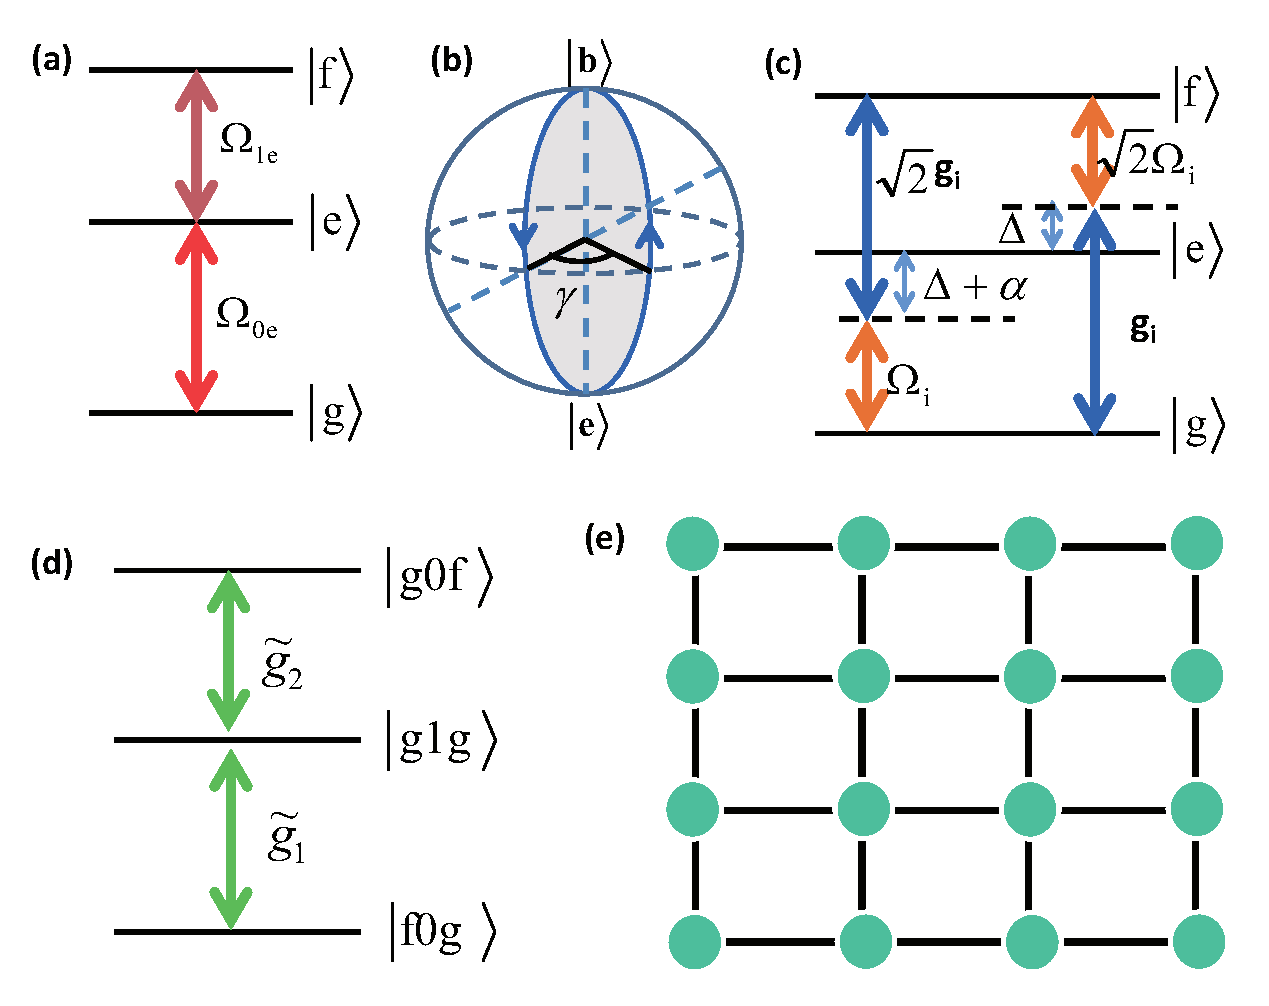
\includegraphics[width=0.7\linewidth]{Figures/transmon/setupnew}
	\caption{我们的单比特和乐门方案的示意图。(a)Transmon量子比特和亮哥微波场耦合。(b)在参数空间中的绕圈方式。(c)两比特门的实现方法。(d)两比特门单激发空间的有效模型。(e)我们的方案的可以拓展到2D阵列。图片来自参考文献\cite{hong2018implementing}。}
	\label{fig:setupnew}
\end{figure}

我们考虑如何在Transmon上来实现任意的上述的和乐门,装置如图\ref{fig:setupnew}。具体来说,我们考虑的是一个$G_2(C^N)$的情况,其中$N$是我们考虑的transmon的可操作的能级,为简便计,我们仅仅考虑$3$个能级,记做$\ket{g}, 
\ket{e},\ket{f}$让高激发态$\ket{f}$和基态$\ket{g}$作为计算空间,两个驱动场分别记做$\Omega_{ie}(t)$ ($i=0, 1$,初始相位为$\phi_i$,Transmon的有效哈密顿可以写作:

\begin{eqnarray} \label{h1}
H_{1} &=& \Omega_{0e}(t)e^{i\phi_0}|g\rangle\langle e|+
e^{i\phi_1}\Omega_{1e}(t)|f\rangle\langle e|  + \mathrm{H.c.}\\
&=&\Omega (t) e^{i(\phi_1-\pi)} \left(\sin\frac{\theta}{2}e^{i\phi}|g\rangle -\cos\frac{\theta}{2}|f\rangle\right)\langle e| + \mathrm{H.c.},\notag
\end{eqnarray}
其中 $\phi=\phi_0-\phi_1+\pi$, $\Omega(t)=\sqrt{\Omega_{0e}(t)^2+\Omega_{1e}(t)^2}$, 且$\tan(\theta/2)=\Omega_{0e}(t)/\Omega_{1e}(t)$. 系统的动力学由这亮态 $|b\rangle=\sin(\theta/2)e^{i\phi}|g\rangle-\cos(\theta/2)|f\rangle$ 和 $|e\rangle$控制, 暗态 $|d\rangle=\cos(\theta/2)|g\rangle+\sin(\theta/2)e^{i\phi}|f\rangle$ 上没有动力学,因此满足了上方程.\ref{eq:require}. 如果循环演化条件也满足了 $\int_0^T \Omega(t) dt=\pi$, 任何单比特门都可以通过选择 $\theta$ 以及 $\phi$得到.同时,因为 $\langle j(t)|H_1|i(t)\rangle=0$ 其中$i\in\{b, d\}$, 因此 $|d\rangle$ 和$|b\rangle$ 之间没有跃迁, 那么$|d\rangle$ 和 $|b\rangle$ 的动力学相位都等于零,即满足了方程\ref{eq:require}。这样得到的量子门,就是和乐门的实现了。

为了得到一系列通用的量子门,或者说检测不同的路径$U(C)$是否构成了一个通用的门,我们让演化时间为两个区间,i.e, $\phi_0=0$, $\phi_1= \pi$ 当 $t\in [0, T/2]$, 以及 $\phi_0'=\pi+ \gamma$,  $\phi_1'= \gamma$  当 $t\in [T/2, T]$. 这种情况下,两个分开的演化路径对应的哈密顿量分别是
 $H_a=\lambda_1(|b\rangle\langle e|+ |e\rangle\langle b|)$ 以及 $H_b=-\lambda_1 (e^{i\gamma} |b\rangle\langle e|+ e^{-i\gamma} |e\rangle\langle b|)$,
 对应的演化算符就是$U_a=|d\rangle\langle d| -i (|b\rangle\langle e|+ |e\rangle\langle b|)$以及$U_b=|d\rangle\langle d| + i (e^{i\gamma} |b\rangle\langle e|+ e^{-i\gamma} |e\rangle\langle b|)$. 因此,单比特门就是,
\begin{eqnarray}\label{singleloop}
U_1(\theta,\phi) &\sim& \left(\begin{array}{cc}
\cos \frac{\gamma}{2}-i\sin\frac{\gamma}{2}\cos\theta & -i\sin\frac{\gamma}{2}\sin\theta e^{i\phi}\\
-i \sin\frac{\gamma}{2}\sin\theta e^{-i\phi} &\cos\frac{\gamma}{2}+i\sin\frac{\gamma}{2}\cos\theta
\end{array}\right) \nonumber \\
&=& \exp\left({-i{\gamma \over 2} {\bf n}\cdot{\bf \sigma}}\right),
\end{eqnarray}
也就是一个绕着轴${\bf n}= (\sin\theta\cos\phi, \sin\theta\sin\phi, \cos\theta)$ 旋转$\gamma/2$的操作,并且可以得到一系列的单比特空间的门操作(确定到一个不重要的相因子的程度 $\exp(i\gamma/ 2)$)且是和乐的。例如,对于 $(\theta, \phi)$, 对应的两类门 (不同的 $\gamma$) 构成了单比特门的一个通用类。从几何的观点,上面的两个哈密顿对应Bloch球上两个不同的路径,并且是分割循环的,两个哈密顿在中间时候相同。得到的几何相位可以用\ref{fig:setupnew}上的分割路径看出。 要注意的是,$\Omega(t)$能够任意的选择,只要他们相同,这是因为我们的模型是共振耦合的,不依赖驱动的形式(只对它有积分为$\pi$的要求)。


\begin{figure}[tbp]\centering
	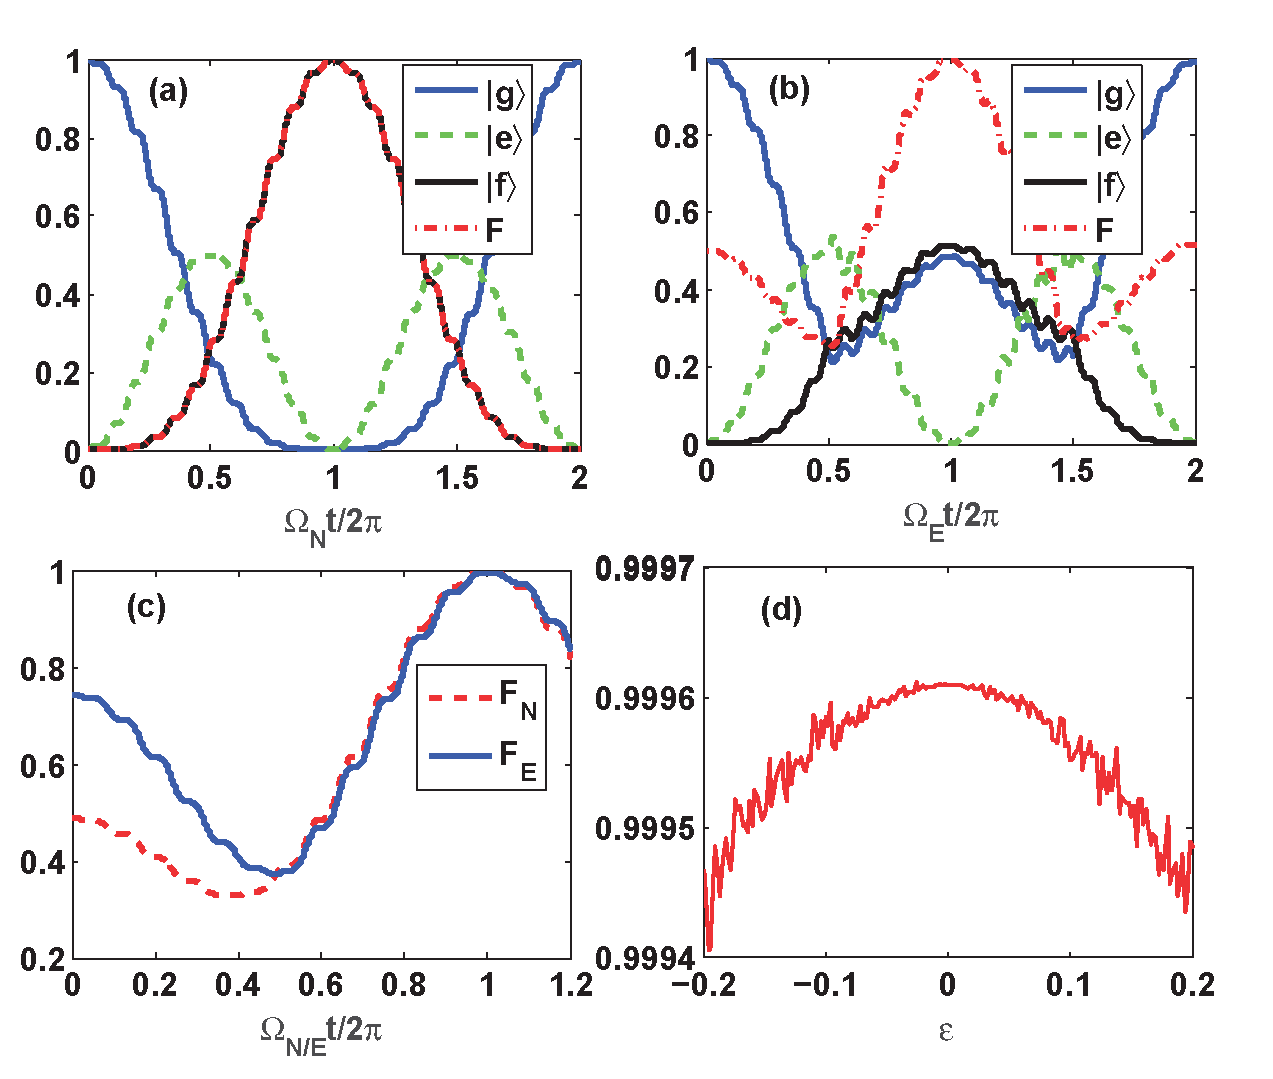
\includegraphics[width=8cm]{Figures/transmon/f1.eps}
	\caption{ $(\gamma, \theta)$ 门的保真度演化,  (a) $(\pi, \pi/2)$ 和 (b) $(\pi/2, \pi/2)$, 作为 $\Omega_{N/E}t/\pi$的函数,其中初态设置为 $|g\rangle$. (c) 门保真度的演化。 (d) NOT门对脉冲扰动$\epsilon\Omega$的稳定性。图片来自参考文献\cite{hong2018implementing}。 }
	\label{Fig f1}
\end{figure}
这样的和乐门还有对噪声不敏感的特征,考虑马尔科夫的噪声,也就是上面式\ref{singleloop}对于的量子主方程:
\begin{eqnarray}  \label{me}
\dot\rho_1 &=& i[\rho_1, H_1]  + \frac{1}{2} \sum_{j\in\{g, f\}} \left[ \Gamma_1^{j} \mathcal{L}(\sigma^-_{j,e}) + \Gamma_2^{j} \mathcal{L}(\sigma^\text{z}_{j,e})\right],
\end{eqnarray}
其中 $\rho_1$  是我们考虑系统的密度矩阵,$\mathcal{L}(A)=2A\rho_1 A^\dagger-A^\dagger A \rho_1 -\rho_1 A^\dagger A$ 是 $A$, $\sigma^-_{g,e}=|g\rangle\langle e|$, $\sigma^-_{f,e}=|e\rangle\langle f|$, 的刘维儿算符,其中$\sigma^\text{z}_{f,e}= (|f\rangle\langle f|-|e\rangle\langle e|)$, $\sigma^\text{z}_{g,e}= (|e\rangle\langle e|-|g\rangle\langle g|)$. 另外
$\kappa$, $\Gamma_1^j$,  $\Gamma_2^j$ 是腔的耗散、$\{j,e\}$ 两个能级的耗散假设系统处在基态 $|g\rangle$,选择NOT门,我们可以用保真度$F=\langle\psi_f|\rho_1|\psi_f\rangle$ 来衡量我们的和乐门,其中$|\psi_f\rangle=|f\rangle$ 且$|\psi_f\rangle=[(1+i)|g\rangle+(1-i)|f\rangle]/2$ 是我们的目标态。如图\ref{Fig f1}(a)和 \ref{Fig f1}(b)所示,
得到的保真度高达 $F _{N}= 99.75\%$ 和$F _{E}= 99.56\%$ ,演化时间$t=\pi/\Omega_{N/E}$.量子比特的参数设置为 $\Omega(t) = 2\pi\times 16$ MHz,  且 $\Gamma_1^j=\Gamma_2^j= \kappa=2\pi \times 10$ kHz,  对应退相干时间 16 $\mu$s,失谐量设置为 $\alpha=\omega_{ge}-\omega_{fe}=2\pi\times 400$ MHz。 我们设置$\Omega_{0e}=\Omega_{1e}= \Omega_{N/E}/\sqrt{2}$ 使得 $\theta = \pi/2$. 
另外,对于一般的初态,
 $|\psi\rangle=\cos\theta^{'}|g\rangle+\sin\theta^{'}|f\rangle$ 其中$\theta^{'}=0$ 对应 $|0\rangle$ 态,得到的保真度只有非常小的改变 $\theta^{'}>0$。图. \ref{Fig f1}(c)我们画了1001个输入态对应 $\theta^{'}$ 在 $[0,2\pi]$均匀的改变, 其中 $F _{N}= 99.82\%$, $F _{E}= 99.57\%$. 为了测试体系对脉冲失稳的健壮度, 我们给脉冲也加上小的随机扰动: $\Omega\to \Omega^{'}=(1+\epsilon)\Omega$, 其中 $\epsilon$ 为一个均值为$0$的分布。 无退相干的情况下,$\epsilon$可以增加到$20\%$,和乐门的保真度也不会大大下降。

 推广到两比特门的办法是直接的,我们可以考虑两个量子比特用一个非线性的腔耦合起来(来避免腔的高光子数激发)并找到一个两比特的子空间,如图\ref{fig:setupnew},有兴趣的读者可以查阅参考文献\cite{hong2018implementing}中的设计。

   \newpage
   \section{量子模拟}
   由于近年来量子系统的完全控制技术的发展\cite{song201710},由费曼提出的量子模拟和量子计算在实验上成为了可能。量子模拟有望成为一个在凝聚态物理、原子分子光物理和化学等学科中有用的理论和实验平台。量子模拟器可以当做一个简易版本的量子计算机,或者说一个\textit{模拟}量子计算机。这一章节我们来介绍量子模拟的基本理论和最新进展\cite{blais2004cavity,you2006superconducting,clarke2008superconducting,Georgescu2014}。
  
  量子模拟器是一种可控的、容易读取的量子系统,用来模拟更加不可控、大型的系统。三十年前,测试物理的量子描述成为了计算物理学家最大的难题——显然,一个巨大的量子系统的尺度在线性增加的时候,参数确实以指数形式增加的。一个可能的解决方案是利用近似办法,例如蒙特卡洛模拟。但是,存在所谓的符号问题,限制了这个方法的适用范围。其他的可能的办法,例如利用张量网络来表示多体波函数,被认为在无能隙的情况下难以近似一个量子体系。
  
  从费曼的视角,他提出了一种新类型的计算机:\textit{让计算机本身就是由服从量子定律的量子元素构成。} \cite{feynman1982simulating}但是他没能明确他的量子计算机如何工作、如何实现。 十年时候,Lloyd提出一个作为量子模拟器的量子比特系综\cite{lloyd1996universal}。在这个框架下,量子比特可以被一些工程手段初始化、测量和控制。
  
  总的来说,去制作一个通用的量子计算机对于物理学家来说还是非常有难度的\cite{harrow2017quantum}。但是物理学家们已经迫不及待地想将这样的量子体系应用在更加实际的问题了。例如,一些物理模型的量子模型已经得到了十足的进展\cite{Georgescu2014}。例如,解析计算一些含有相互作用的多体哈密顿量目前还是非常有难度的,例如Mott-Hubbard模型\cite{inguscio2008ultra}、t-J模型\cite{lee2006doping}和量子自旋链模型\cite{giamarchi2003quantum},但是利用量子模拟技术,这些模型中的量子物相\cite{sachdev2007quantum}、纠缠特征和拓扑特性\cite{zeng2015quantum}已经可以期待使用一个具有量子特性的模拟器找到了\cite{harrow2017quantum}。
  
  当然,为了让我们获得一种不仅仅使得物理学界获益,而使得日常生活中方方面面都受益的技术,我们不能满足于现有的成就。通过比较量子模拟的结果和精确可解的模型,我们对我们的模拟器的量子特性充满了自信,然后我们就应该去制作一个量子计算机了,量子计算的计算能力增长也服从一些摩尔定律,如图.\ref{fig:moore}所示。通过物理学家们的努力和创造,量子计算应该能在某一个特定的实践性的方面能够超出任何的超级计算机。这就是\textit{量子霸权}\cite{harrow2017quantum}。
  
  潜在量子模拟和量子计算的物理实现平台包括\cite{Georgescu2014}:固体系统中的缺陷(例如NV色心\cite{childress2006coherent}),离子阱\cite{leibfried2003quantum},中性冷原子(分子)\cite{demille2002quantum},光学腔\cite{imamog1999quantum},光子学体系\cite{o2009photonic},光子体系\cite{knill2001scheme},量子点\cite{hanson2008coherent},超导量子电路和核自旋体系。基于各个平台不同的优势和缺点,它们可以用于不同的任务。例如,因为超冷原子的可扩展性,这个平台可以被视作研究多体现象的最佳平台\cite{bloch2008many}。由于超导量子电路扩展性和可控性的进展,这个平台被视作最有可能实现量子计算的平台\cite{blais2004cavity}。其他的平台可以在量子测量\cite{giovannetti2006quantum}、量子传感\cite{degen2017quantum}、精密测量\cite{giovannetti2011advances}、化学\cite{lanyon2010towards}、生物\cite{wu2016diamond}和医学\cite{bailey2004quantum}找到自己的应用地位。
        \begin{figure}
  	\centering
  	\includegraphics[width=0.9\linewidth]{Figures/review/Moore}
  	\caption{量子计算的摩尔定律。来自参考文献\cite{GU20171}。}
  	\label{fig:moore}
  \end{figure} 
   
   \subsection{量子模拟的纲领}
   我们首先考虑一个更加不可控的量子体系,其哈密顿量记做$H_{\text{sys}}$记目标希尔伯特空间的态矢量为$\ket{\psi}_{\text{sys}}$。由于量子力学理论,初态$\ket{\psi(t_0)}_{\text{sys}}$到末态$\ket{\psi(t)}_{\text{sys}}$的演化是幺正的,并且记做$U\left( {t,{t_0}} \right) = \mathcal{T}\left\{ {\exp \left[ { - i\hbar {H_\text{sys}}\left( {t - {t_0}} \right)} \right]} \right\}$其中$\mathcal{T}$是编时算符。
   
一个更加可控的系统从态${\left| {\phi \left( t_0 \right)} \right\rangle _{sim}}$ 演化到 ${\left| {\phi \left( t \right)} \right\rangle _{sim}}$,通过演化算符 
   $\tilde U\left( {t,{t_0}} \right) = \mathcal{T}\left\{ {\exp \left[ { - i\hbar {H_{sim}}\left( {t - t_0} \right)} \right]} \right\}$. 因此,如果存在一个从原来系统到量子模拟器上的映射,
   这个系统就可以按照图.\ref{fig:quantumsimu}的方法模拟\cite{Georgescu2014}。

\begin{figure}
	\centering
	\includegraphics[width=1\linewidth]{Figures/mine/1}
	\caption{量子模拟的图像。被模拟的系统在灰色方框中,这个系统是难以获取、或者难以控制的。一个良定义的模拟器因为着,它的初始态可以被制备出来,态的演化可以操控,并且末态可以测量。在把原来的系统和现有的系统映射之后,我们就从模拟器中获取信息了。由于两个系统满足同样的物理定律,获取的信息可以被映射回原来的系统。}
	\label{fig:quantumsimu}
\end{figure}
   
   用数学语言来说,一个模拟器的哈密顿量可以写作:
      \begin{equation}
   \begin{gathered}
   {H_{\textbf{sim/sys}}} = {H_0} + {H_d}\left( t \right) \hfill \\
   {H_0} = \sum\limits_{i,j,m,n} {v_{m,n}^{i,j}{{\left( {a_i^\dag } \right)}^m}{a_j}^n}  \hfill \\
   {H_d} = \sum\limits_{i,j,m,n} {u_{m,n}^{i,j}\left( t \right){{\left( {a_i^\dag } \right)}^m}{a_j}^n}  \hfill \\ 
   \end{gathered} 
   \end{equation}
   其中 $a_i,a_i^{\dagger}$ 分别表示产生和湮灭算符。$H_0$ 是模拟器的哈密顿量,并且是固定的,$H_d$是人工的哈密顿量,这个哈密顿量可以被调控,因此这个系统是更加可控的\cite{Georgescu2014}。绝大多数的模拟器的模型和原本系统的模型可以被这个语言描述。为了模拟一个量子系统,量子模拟器的希尔伯特空间一般要比真实系统的希尔伯特空间要大。然后,保证$a_i$ 和 $\tilde{a}_j$的对易关系,我们可以给出映射: $\vartheta :v\left( u \right)_{m,n}^{i,j} \to \tilde v\left( {\tilde u} \right)_{m,n}^{i,j}$。有几种不同的量子模拟的类型,因为不同他们的模拟过程和驱动哈密顿背后的思考非常不一样\cite{Georgescu2014}。
   
   \emph{数字型量子模拟(DQS,Digital Quantum Simulation) }只是需要单比特门和两比特非平庸的门。 
   波函数是编码在量子比特中的,并且复杂的幺正演化都被Trotter分解为单比特门和两比特门的序列。 因为DQS有潜力实现任意的幺正演化,DQS是通用的。但是这并不意味这他就是通用量子计算机,由于保真度问题,并不是所有的幺正演化都可以在多项式模拟,因此DQS只能被当做量子算法的简单模拟器。数字型量子模拟的量子比特一般来自体系多个能级的二能级子空间。由于二能级量子比特和其他的能级的能量差很大,因此来自其他能级的影响可以和环境的退相干一并考虑。 我们刚刚展示了Transmon比特里面的和乐量子门可以有效的减少不同能级之间的跃迁和控制脉冲的失稳${H_d}\left( {\Omega \left( t \right)} \right) \to {H_d}\left( {\Omega \left( t \right) \pm \varepsilon } \right)$,因此这个办法可以用来完成高保真度的数字型量子模拟的实验。
   
   按照前面讨论的量子模拟的精神,数字型量子模拟可以分作下面的步骤\cite{Georgescu2014}:
   \begin{enumerate}
   	\item 初态的制备。初态的制备的方法有很多,见。值得提及的是,初态的制备被证明是可以在多项式级别完成的。
   	\item 幺正演化。考虑要模拟哈密顿量是一系列多体算符的求和,$H = \sum_m H_m$,对应的幺正演化,由于$[H_m,H_n] \ne 0$,我们无法做分解$U \ne \prod_m \exp(-i H_m t)$,但是如果我们如果采取时间上一段一段的演化$U(dt) = \prod_m \exp(-i H_m dt) + O(dt^2)$则是可行的。但是随着精度的提高,我们需要非常大量的量子门,这可能导致低效甚至DQS的失效。
   	\item 测量。 在进行幺正演化之后我们最重要的就是测量并提取我们的信息例如$\avg{A^\dagger B}$,一个简单的办法是测量所有的态矢量分量,这个办法就是量子态断层成像技术。但是量子态的维数是随着体系的尺度指数上升的,这样的办法很快就会失效。上一节我们作为例子引入了超导量子电路中的谱测量办法,这样的办法就是一种避免量子态层析成像的途径。
   \end{enumerate}

   
   \emph{模拟型量子模拟(AQS,Analog quantum simulation)} 模拟型的量子模拟是自然但是不通用的办法。 一个不可控的哈密顿量直接被映射到另一个系统。不像DQS中我们把幺正演化分割成量子门,我们在AQS用哈密顿量来实现模拟,一次你,AQS本身就是有个具有有效哈密顿的多体体系。及时这个系统在某些参数不能很好的控制,我们也能测量一些稳定的数值和现象,例如相变、拓扑效应等等。这些效应可以不同程度上回答不同类型的多体里的问题。但是事实上,有的时候找到真正的哈密顿量之间的映射是非平庸的问题\cite{Georgescu2014}。
   
   AQS的一个好处是,一切耗散都是知晓的,因此只要两个系统直接的映射没有全局依赖\footnote{例如Jordan-Wigner 变换就是全局性的变换,而Holstein-Primakoff 变换则是局域的。},那么一般来说耗散也就是局域的。由于相变等等物理现象是具有局部微扰的稳定性的,那么耗散不大的时候体系的相变依然能够看到。而在DQS中,由于使用了Trotter分解,这个映射关系变得不明朗\cite{Georgescu2014}。
   
   
   \subsection{应用1:超导量子电路模拟拓扑绝缘体}
  物理中拓扑物态的研究始于量子霍尔效应\cite{laughlin1981quantized},拓扑物态在凝聚态物理学中扮演了重要的地位\cite{RevModPhys.83.1057}。 自然界中已经有非常多的拓扑绝缘体\cite{fu2007topological}和拓扑超导体被发现了\cite{Ando2013topological,ando2015topological,yuan2014generation},这些拓扑绝缘体和拓扑超导体可能在自旋电子学\cite{murakami2003dissipationless,koralek2009emergence}和
  拓扑量子计算中发挥作用\cite{sau2010generic,Laughlin1983}。进一步,现有的原子分子光物理等等最新的技术也允许我们去利用AQS去模拟这些新奇的物态。这个想法已经在光子学\cite{khanikaev2013photonic,ozawa2018topological,schomerus2013parity,yang2018ideal,cheng2016robust}、磁子学\cite{zhang2013topological,mochizuki2014thermally}、超冷原子\cite{Goldman2010,Grusdt2014,Goldman2014,aidelsburger2011experimental,Zhai2015,Wang2010}、线性电路\cite{Whittaker2018,Ningyuan2015,Zhu2018}和超导量子电路\cite{Ashhab2014}等等\cite{Sala2015a}。由于这些实验上的进展,拓扑物态的特征可以以一种更加清晰的方式呈现在我们面前,例如零模、费米电、费米环,它们可以以一种相比固体系统更加清晰的方式呈现在我们眼前\cite{hsieh2009observation,imhof2018topolectrical,Wu2006}。这些成果进一步的加深了我们对拓扑物态的理解,并且可能有全新的应用\cite{aidelsburger2015measuring}。
  
  这一小结我们着重介绍我们使用超导量子电路模拟拓扑绝缘体的进展,最后我们简介一下我们最近在这个的基础上发现的一些非厄米的物理,这可能带来拓扑物理的新的变革。
  
  凝聚态的着重研究点在图.\ref{fig:cmt}中已经展示出来了,纵轴没有意义仅仅是为了方便展示,横轴是体系的特征尺度,可以用能标的倒数来刻画。从左向右看,能标不断提高。首先,在最高能的情况下,起到主要作用的是体系的微观结构。例如体系的基本构成是什么类型的原子等等。在量子模拟体系中,我们有时可以从微观层面上就去控制物质,所以有时候我们也把量子模拟的模拟器叫做人工物质。这些细节已经不再是凝聚态研究的核心主题了。随着特征尺度的加大,我们首先看到横贯所有能标的就是体系的维度。维度起作用的主要方式,是因为各个维度的自由格林函数的性质大不相同,而自由格林函数在系统的热力学、响应、输运等等一系列性质中都扮演了核心的角色,因此维度几乎一直都起作用。另外看到对称性和拓扑。这里的对称性和拓扑都是体系的宏观对称性和拓扑,例如体系满足怎样的晶体群,是否满足时间反演对称性(TRS,$\mathcal{T}$)等等。有一些对称性还是演生的,是一些准粒子表现出的特殊性质,最典型的例子就是BCS理论中的波戈留波夫准粒子,表现出来了粒子-空穴对称性(PHS,$\mathcal{P}$),还有一个很容易存在在凝聚态系统中的对称性,它是手征对称性(CS,$\mathcal{P}$)。可以证明,具有$\mathcal{P}$和$\mathcal{T}$对称性的系统一定具有$\mathcal{C} = \mathcal{PT}$手征对称性。然后是拓扑。我们看到拓扑和体系的对称性有一块重叠,也就是拓扑存在与否其实和体系的对称性有关,完整的给出这个问题的回答的是利用$K$理论建立的十重分类技术。也存在不依赖任何对称性就具有拓扑性质的系统,例如拓扑绝缘体中的$A$类,一个典型的例子就是量子霍尔效应不需要任何的对称性去保护,见\ref{sub3}节。
\begin{figure}
	\centering
	\includegraphics[width=1\linewidth]{Figures/topoinsu/cmt}
	\caption{当今凝聚态研究的主题。从Mircroscopic Detail: 微观细节,到Symmetry: 对称性,topology: 拓扑,Dimensionality: 维度, 以及近年来刚刚兴起的Hermicity: 厄米性和Gauge:规范势。}
	\label{fig:cmt}
\end{figure}

近年来,厄米性和规范不变性也加入了凝聚态这个宏大主题的讨论之中,进一步丰富了凝聚态物理的研究内容\cite{Gong2018topo,malzard2015topologically,lourencco2018self,esaki2011edge,Shen2018,Osterloh2005,Goldman2009,zeuner2015observation,leykam2017edge,lee2016anomalous,yuan2014generation,Wu2015,sau2010generic,ozawa2018topological,Wu2013,feng2017non,Yao2018,Yao2018a}。我们最后会稍微提及厄米性,但是规范场和拓扑会一直是本节研究的主题。

第一个研究规范场和拓扑之间关系的是Hofstadter模型\cite{rammal1985landau,Galitski2013,claro1979magnetic,Ningyuan2015,hofstadter1976energy,owens2018quarter,Osterloh2005,Wu2015,aidelsburger2013realization,aidelsburger2015measuring},它来自于二维磁场中自由电子的朗道能级的研究\cite{aidelsburger2011experimental}。
考虑如下哈密顿量,它是二维磁场中自由电子的格点版本\cite{claro1979magnetic},同时选择朗道能级和特殊的磁通,我们有:
\begin{equation}
H = -J\sum_{m,n} a^\dagger_{m,n+1} a_{m,n} + e^{-i \Phi} a_{m+1,n}^\dagger a_{m,n} + h.c, \Phi = 2\pi \frac{p}{q}
\end{equation}
\begin{figure}
	\centering
	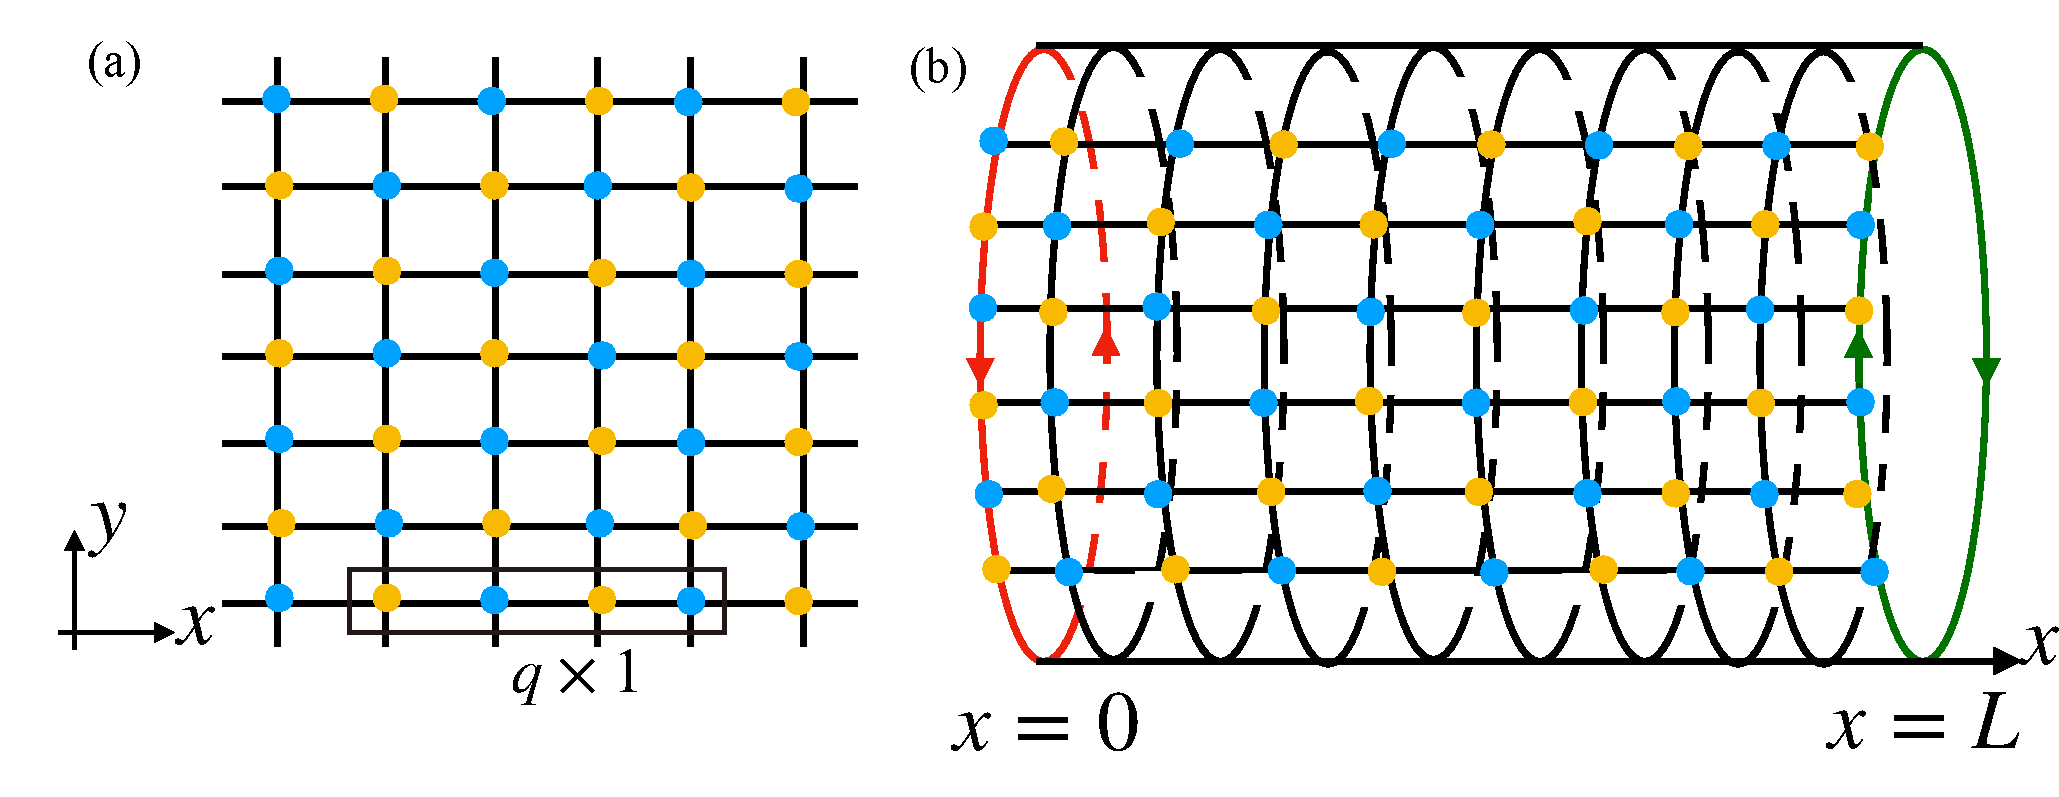
\includegraphics[width=1\linewidth]{Figures/topoinsu/SP6}
	\caption{两种对角化的空间。(a)一个无穷大的系统。(b)将无限大的系统($T^2$)裁成一个圆柱$S^\times [-1,1]$}。
	\label{fig:sp6}
\end{figure}

我们分别在下图的两种几何状况下对角化我们的哈密顿量,如图,在磁倒格子(Magnetic BZ, MBZ)中进行傅里叶变换,我们可以得到:
\begin{equation}
-2J\cos(k_x + n\Phi) a_n - J(e^{-i k_y}a_{n-1} + e^{i k_y}a_{n+1})=Ea_n
\end{equation}
如果是圆柱结构的,我们可以得到一个好量子数:
\begin{equation}
H(m,k_y) = -Ja^\dagger_{m+1}a_m-2J\cos(k_y-\Phi m)  a_{m}^\dagger a_m
\end{equation}

我们于是可以得到体系的能谱。在Hofstadter模型里,当q是偶数的时候,我们在$E\approx 0 $附近有一些简并的狄拉克费米子,如图\ref{fig:band}所示。

\begin{figure}
	\centering
	\includegraphics[width=0.7\linewidth]{Figures/topoinsu/band}
	\caption{Hofstadter模型在圆柱几何下的能谱,我们可以看到无能隙的狄拉克费米子和一些激发态。由于有两个边缘,陈数为1,每个边缘贡献一条边缘态。}
	\label{fig:band}
\end{figure}

可以这样理解这些边缘态,因为Hofstadter模型是朗道能级的分立结构,而我们知道对于朗道能级$C_n = -1$,对于Hofstadter模型,它的高能激发确实满足朗道能级
的平带特征,因此高能的激发也具有$C_n = -1$,因此gap中获得了非平庸的陈数,因此有限大的体系边界会有边缘态。

值的一提的是这个体系在MBZ的哈密顿量具有隐藏的手征对称性\cite{wen1989winding},哈密顿量可以变形写作:
\begin{equation}
H = e^{-ik_x} V + e^{-ik_y} S + h.c.
\end{equation}
其中 $V = \text{diag}(e^{-2\pi i pn/q})$, $S^n = I$, $S^\dagger S = I$.

定义 
\begin{equation}\label{eq:Gamma}
\Gamma = (-1)^j (i)^{q/2} \delta_{j,j+q/2}
\end{equation}
我们发现 :
\begin{equation}
\{\Gamma, V\} = \{\Gamma, S\} = \{\Gamma, H\} = 0, \quad \Gamma^2 = I
\end{equation}
因此, $\{\Gamma,H\} \psi_n = 0 \to H(\Gamma\Psi_n) = -E_n (\Gamma \psi_n)$

在这个基下, $U$ 由 $\Gamma = U (\Sigma_z \otimes I) U^\dagger$定义, 我们有:
\begin{equation}
U H U^\dagger = \left(\begin{array}{cc}
& q \\ 
q^\dagger & 
\end{array} \right)
\end{equation}
因此$\text{det} H = -\text{det} q^\dagger q$. 哈密顿量 $H$的同伦不变量就可以写作 $$v  = \frac{1}{4\pi i} \oint_c \Gamma H^{-1} d H$$,非零的环绕数决定了体系能谱中间的Dirac费米子的稳定性。

我们接下来在这个基础上来构造拓扑绝缘体。由于这个体系破坏了时间反演不变形,因此我们可以考虑增加分量来构造时间反演不变的系统\cite{Wu2013,Wu2015}:
\begin{equation}
\tilde{H} = \left(\begin{array}{cc}
H &0  \\ 
0& \mathcal{T}H\mathcal{T}^{-1}
\end{array} \right)
\end{equation}
如果在斜对角元加上耦合(自旋轨道耦合,SOC),但是不打破时间反演对称性,并不关闭能隙,可以证明此时的系统属于QSH相。这种扩展,加上SOC也可以看成一个非阿贝尔规范场。
以此为出发点,我们考虑如图\ref{fig:fig1}所示的系统,每个格点上有一个带自旋的人工的波色激发,它的哈密顿写作:
   
\begin{figure}
	\centering
	\includegraphics[width=1\linewidth]{Figures/topoinsu/fig1}
	\caption{我们考虑的系统:(a)我们考虑的系统包括一个多分量格点阵列和一个测量装置。(b)$U_y$为$y$方向的跃迁矩阵。(c)$U_x$为$x$方向的磁场。(d)每个格点上是一个3D腔,我们考虑它的两个模式。}
	\label{fig:fig1}
\end{figure}

\begin{equation}
{\mathcal{H}_0} =  - \sum\limits_{{\bf r}, \sigma = x, y} t_\sigma \psi _{{\bf r} + {\bf e}_\sigma }^\dag U_{{\bf r}}^\sigma {\psi _{{\bf r}}} + \text{h.c.}, 
\label{Eq:main_h}
\end{equation}
其中 ${\psi _{\bf r}} = {\left( {{a_{{\bf r}, \uparrow }}, {a_{{\bf r}, \downarrow}}} \right)^T}$表示(赝)自旋的场算符 , $t_\sigma$ 是最近邻的朝着 $\sigma$ 方向的跃迁强度, ${\bf e}_x = (1,0)$,${\bf e}_y = (0,1)$.我们的工作中,我们想要去探究非阿贝尔规范场$\mathcal{A} = - (2\pi \gamma \sigma_x, 2\pi \alpha x \sigma_z)$,它的晶格模型可以写作
\begin{equation}
\label{eq:hopping}
U_{{\bf r}}^x= U^x = {e^{i{\Theta _x}}}, \quad U_{{\bf r}}^y=U^y_r=e^{i{\Theta _y}},
\end{equation}
其中 ${\Theta _x} = \gamma  \cdot 2\pi {\sigma _x}$, 且${\Theta _y} = \alpha  \cdot 2\pi m{\sigma _z}$, 其中$(x,y)= (m,n)$.

\begin{figure}
	\centering
	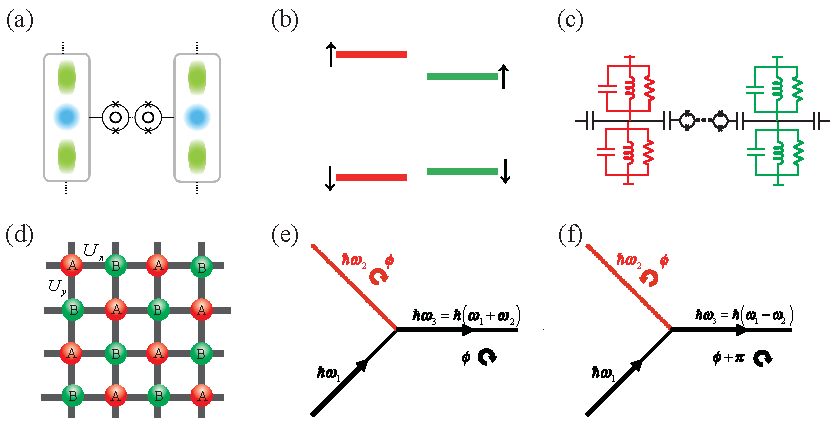
\includegraphics[width=1\linewidth]{Figures/topoinsu/S7}
	\caption{(a)我们考虑两个3D腔作为我们模型的小模块\cite{Paik2011,Girvin2013,reagor2013reaching},其中两个最低的模式如图(b)所示。 (c)体系的等效RLC回路,(d)这些腔可以被拓展到一个阵列。(e.f)两种不同的参变过程。}
	\label{fig:s7}
\end{figure}
为了讨论如图\ref{fig:s7}所示的体系实现非阿贝尔的规范场\cite{Goldman2009},我们首先考虑一个两个格点的问题,它的哈密顿量是\cite{Zakka-bajjani2011}:
\begin{equation}
H_\text{two-sites} = \sum_{\sigma = \uparrow / \downarrow , i = 1,2}\omega_{\sigma,i} n_{\sigma,i} + 2{\bf{t}} \sum_{\sigma, \sigma'} \cos(\Delta_{\sigma 1,\sigma' 2} t + \phi_{\sigma 1,\sigma' 2})
\end{equation}
旋转表象下,我们定义:
\begin{equation}
U = \exp \left\{-i t \left[ \sum_{\sigma = \uparrow / \downarrow , i = 1,2}\omega_{\sigma,i} n_{\sigma,i} -2 \lambda(n_{\uparrow,1} + n_{\downarrow,1}) \right]\right\}, 
\end{equation}
因此我们的有效哈密顿量就是:
\begin{equation}
\begin{aligned}
\tilde{H} &= U^\dagger H_{\text{Real}} U + i (\partial_t U^\dagger )U \\
&= 2 \lambda (n_{\uparrow,1} + n_{\downarrow,1}) + {\bf{t}} \sum_{\sigma, \sigma'} \left[e^{i(\Delta_{\sigma 1,\sigma' 2} t + \tilde \phi_{\sigma 1, \sigma' 2})} + h.c. \right]\\
&\times\left[ e^{i (\omega_{\sigma,1}-\omega_{\sigma,2} - 2\lambda)t} a_{\sigma,1} a^\dagger_{{\sigma',2}} + h.c\right]
\end{aligned}
\end{equation}
其中 $\tilde \phi _{\r',\r,\sigma ,\sigma '} = \text{sign} (\omega_{\r',\sigma '} - \omega_{\r,\sigma }) \phi _{\r',\r,\sigma ,\sigma '}$.上面的方程中,快速震荡项的周期远远小于$t$和$\lambda$对应的周期,因而是可以忽略的。我们选择${\Delta _{\r\sigma ,\r'\sigma '}}\left( t \right) = \left| {{\omega _{\r,\sigma }} - {\omega _{\r',\sigma '}}} +2\lambda\right|$.,得到了如下的哈密顿量。
\begin{equation}
H_{\text{eff}} = \lambda n_1  - \lambda n_2 +  ({\bf{t}} \psi^\dagger_1 \Phi_{1,2} \psi_2 + \text{h.c.}).
\end{equation}
我们可以用不同的初始条件的粒子的运动来表述上面的过程,我们发现$H_\text{two-sites}$和$H_\text{eff}$会给出同样的动力学。同样的特征也可以在其他的测量试验中观测到,和初始状态无关。

知道了如何在超导量子电路上实现这个模型之后,我们可以专注于这个模型本身的性质。哈密顿量:
\begin{equation}
{\mathcal{H}_0} =  - \sum\limits_{{\bf r}, \sigma = x, y} t_\sigma \psi _{{\bf r} + {\bf e}_\sigma }^\dag U_{{\bf r}}^\sigma {\psi _{{\bf r}}} + \text{h.c.}, 
\end{equation}
取 $\alpha=p/q$, 其中 $p$, $q$ 互质, 我们就可以在MBZ里面对角化这个哈密顿量,得到下面的Haper方程
\begin{equation}
\label{Eq:Haper}
\begin{aligned}
- {t_x}{{\tilde U}^{k_x^0 + 2\pi \alpha n}}{u_n} - {t_y}( {{{\tilde U}^{{k_y}}}{u_{n + 1}} + {{\tilde U}^{{-k_y}}}{u_{n - 1}}} )  = Eu_n,
\end{aligned}
\end{equation}	
其中 ${{\tilde U}^{{k_x}}} ={e^{ - i{k_x}}}{U_x} + \text{h.c.}$, $\tilde U ^{k_y} = e^{-ik_y \sigma_z}$, 且 ${u_n} = {\left( {{u_{n, \uparrow }},{u_{n, \downarrow }}} \right)^T}$,
其中$u_{n, \sigma}$ 是第$n$个分量的波函数的振幅且 $n = 1,2,\cdots, q-1$. 边界条件是 $u_{q} = {u_0}$ , $k_x^0 \in [\frac{-\pi}{q}, \frac{\pi}{q}]$ 且 
$k_y\in [\pi,\pi]$.

下面考虑$y$方向上的哈密顿量:
\begin{equation}
\label{eq: ky}
-t_x[ U^x u_{m+1} + {(U^x)^\dagger} u_{m-1}]-t_y(e^{ik_y}U^y_m + \text{h.c.})u_m = Eu_m.
\end{equation}

对角化得到如图\ref{fig:fig2}所示的能谱结构。
\begin{figure}
	\centering
	\includegraphics[width=1\linewidth]{Figures/topoinsu/fig2}
	\caption{我们画出来了不同磁通下的能谱(Laughlin's argument),这和阿贝尔情况下的能谱完全不一样。}
	\label{fig:fig2}
\end{figure}

我们看到了和阿贝尔情况下的能谱不一样的特征,我们下面来检查Hofstadter蝴蝶谱的情况,对于阿贝尔的情况,如图\ref{fig:sp4}所示,
蝴蝶谱的能隙是稳定的,因此其中的边缘模式可以根据Laughlin泵浦得到。
\begin{figure}
	\centering
	\includegraphics[width=1\linewidth]{Figures/topoinsu/SP4}
	\caption{体系在阿贝尔势能下的能谱,由于没有层和层之间的耦合,体系在不同的$q$情况下有不同的能隙。}
	\label{fig:sp4}
\end{figure}

但是对于非阿贝尔的情况,如图\ref{fig:sp5}所示,蝴蝶谱的能隙反复的关闭和打开,这样,如果存在边缘的模式,体系会在不同的$k$点不断的被湮灭,换一句话说
就是体系任何时候都是处于无能隙的。


\begin{figure}
	\centering
	\includegraphics[width=1\linewidth]{Figures/topoinsu/SP5}
	\caption{体系在非阿贝尔势能下的能谱,由于体系有层和层之间的耦合,体系是无能隙的。}
	\label{fig:sp5}
\end{figure}
我们也可以在MBZ中画出体系的能谱,如图\ref{fig:sband}所示。我们发现体系在$q = 5$也就是$q$为奇数的时候也有无能隙的Dirac费米子,这是因为体系奇数维度虽然没有手征对称性,
但是由于我们是自旋$1/2$体系,系统总得获得了一个对称性。而$q=6$也就是$q$为偶数的时候体系有对称的无能隙的Dirac费米子,它是由轴对称性保护的。
\begin{figure}
	\centering
	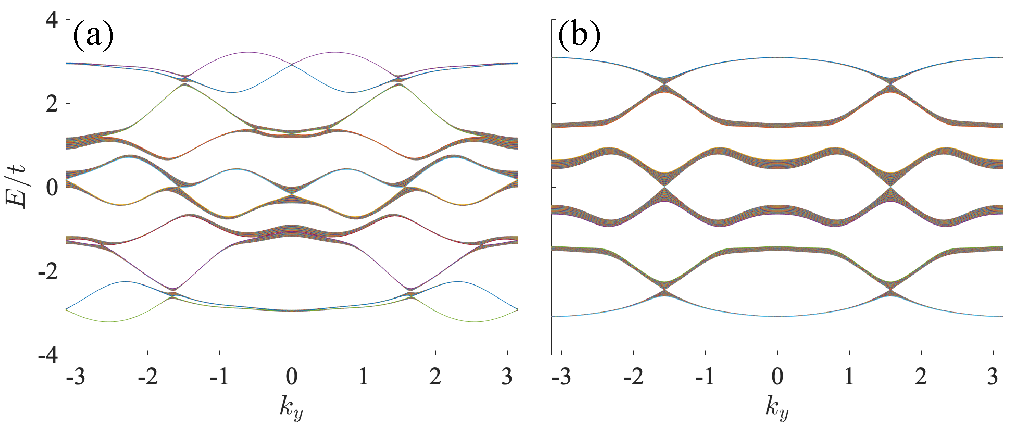
\includegraphics[width=1\linewidth]{Figures/topoinsu/S_band}
	\caption{体系在MBZ中的能谱。(a)$q = 5$,体系在电中性点附近有4个被扭转对称性保护的非手征的狄拉克费米子。(b)$q=6$体系在电中性点有两个高度简并的狄拉克费米子。}
	\label{fig:sband}
\end{figure}
对于$q$为偶数,我们的体哈密顿量可以写作:
\begin{equation}
H_h = \tilde{U}^{k_y} \otimes S +  V_s \otimes S^3 + \text{h.c.}+V
\end{equation}
其中 $V = \text{diag}(U^{k_x + 2\pi n/q})$, $n = 1,...,6$. 
体系的手征算符现在写作:

\begin{equation}
\Gamma \rightarrow \Gamma \otimes I_2,
\end{equation}
其中,原本无自旋的手征算符 $\Gamma = (-1)^j (i)^{q/2} \delta_{j,j+q/2}$ 被替换成了一个SU$(2)$的版本。

整个体系的哈密顿量还有一个对称性,也就是时间反演对称性,
\begin{equation}
\mathcal{T} H(-k) \mathcal{T}^{-1} = H(k)
\end{equation}
因此我们有四重简并的狄拉克点以及两个简并的Dirac费米子。

为了得到QSH,我们可以打破体系的轴对称性,考虑下面的势能:
	\begin{equation}
\label{Eq:Potential}
\mathcal{V}_{\text{s}} = \sum_{\bf r} {\left( {-1} \right)^{r_x}}{\lambda}\psi _{{\bf r}}^\dag {\psi _{{\bf r}}}.
\end{equation}
\begin{figure}
	\centering
	\includegraphics[width=1\linewidth]{Figures/topoinsu/fig3}
	\caption{(a)无耦合的时候,体系是无能隙且有QSH相的。(b)有耦合,$q$为偶数,体系被打开了一个有限大小的能隙里面有QSH相对应的边缘态。}
	\label{fig:fig3}
\end{figure}
现在,在十重分类中,我们有$\mathcal{C} = 1 , \mathcal{P} = 1, \mathcal{T}  = -1$因此这个系统处于DIII 类,因此是用$Z_2$拓扑不变量标记的。
\begin{figure}
	\centering
	\includegraphics[width=0.7\linewidth]{Figures/topoinsu/SP1}
	\caption{(a)体系在没有上下自旋分量的耦合的时候可以看成两个反向的量子霍尔效应,我们可以通过在(c)在边缘泵浦下分量体系激发了边缘模式,(d)在边缘泵浦上分量,体系激发了边缘模式且能够在边缘绕开缺陷继续传播,(f)在体中泵浦光子,证明体系处于绝缘态。 (b)上下有耦合的时候,我们通过打破体系的轴对称性从而实现自旋霍尔态,(f)((g))激发体系的一个偏激化模式得到向左(右)传播的边缘态。(h)激发体态证明体系处于绝缘态。}
	\label{fig:sp1}
\end{figure}

我们在超导量子电路中可以通过激发对应的边缘模式来观察体系的拓扑性质,如图\ref{fig:sp1}所示。这样我们就实现了拓扑绝缘体的模拟和测量。

这样的使用超导量子电路去模拟拓扑绝缘体是典型的AQS\cite{Wang2016},但是有一个非常有趣的是,我们的体系还能实现通常体系中无法看到的超强的SOC导致的拓扑效应。

但是超导量子电路是一个人工的自身就带有耗散的体系,一般而言,如果耗散太强一般就看不到体系的拓扑性质了,因此光子学体系去实现拓扑绝缘体一般被认为有耗散这样一个无可避免的缺陷。

然而下一节我们会指出,光子学体系中,利用耗散和激励,我们能够实现不一样的拓扑物态,即非厄米下的拓扑物态。
   \subsection{应用2:超导量子电路研究非厄米下的拓扑物相}
   光子学体系一般有不可避免的耗散\cite{regensburger2012parity},一般认为过于强的耗散会让体系失去拓扑性质\cite{st2017lasing},然而,我们指出了非厄米的光子学体系中可能有更加新奇的拓扑相。当这种非厄米和规范场结合在一起\cite{Gong2018topo,malzard2015topologically,lourencco2018self,esaki2011edge,Shen2018,Osterloh2005,Goldman2009,zeuner2015observation,leykam2017edge,lee2016anomalous,yuan2014generation,Wu2015,sau2010generic,ozawa2018topological,Wu2013,feng2017non,Yao2018,Yao2018a},我们就能探究这种
   有趣的新的拓扑相了\cite{harari2018topological}。
   
   我们首先来考虑如何在超导量子电路系统中实现有效的激励和耗散,我们考虑下面的更加通用的模型,体系是$H = \frac{P^2}{2m}$动能的产生湮灭算符表示(因而是$a_\r,a_\r^\dagger$的二次型):
   
   \begin{equation}
   H = \sum_{{\bf r},{\bf r'}} t_{{\bf r},{\bf r'}} a_{\bf r}^\dagger a_{\bf r'},
   \end{equation}
   对应的Markovian Lindblad主方程是:
   \begin{equation}
   i\dot{\rho} = [H,\rho] + \underbrace{i \sum_\alpha \mathcal{L}_\alpha \rho \mathcal{L}_\alpha^\dagger - {i \over 2} \{\mathcal{L}_\alpha^\dagger \mathcal{L}_\alpha, \rho\}}_{\mathcal{L}_{\text{d}}} 
   \end{equation}
   其中$\mathcal{L}_\alpha$ 是体系的耗散算符。我们考虑两种基本的耗散,粒子注入和粒子耗散: $L^+_{\r} = \sqrt{\gamma^+} a_{\r}^\dagger$ 以及 $L^-_{\r} = 
   \sqrt{\gamma^-} a_{\r}$,.
   为了得到体系想干态的演化,我们可以求场算符的均值,i.e,
   \begin{equation}
   \label{eq: Supp8}
   i\frac{d\left\langle a_{\r}\right\rangle }{dt}  = i \text{Tr}[a_\r \dot{\rho}] = \text{Tr} [ a_{\r}H\rho - a_{\r}\rho H + i a_{\r} \mathcal{L}_{\text{d}}]
   \end{equation}
   我们可以得到:
   \begin{equation}
   \text{Tr} [a_{\r}H\rho - a_{\r}\rho H] = \text{Tr} (\rho [a_{\r}, H]) = \sum_{\bf r'} t_{{\bf r},{\bf r'}} \langle a_{\bf r'} \rangle,
   \end{equation}
   这个对玻色子和费米子都是成立的。对于耗散项,我们有下面两个性质:
    \begin{equation}
   \begin{aligned}
   && \text{Tr}\sum\limits_{\r'} {\left[ {{a_\r}{a_{\r'}}\rho {a_{\r'}}^\dag  - \frac{1}{2}{a_\r}a_{\r'}^\dag {a_{\r'}}\rho  - \frac{1}{2}{a_\r}\rho a_{\r'}^\dag {a_{\r'}}} \right]}\\ 
   &&= \frac{1}{2}\text{Tr}\sum\limits_{\r'} {\left[ {{a_{\r'}}^\dag {a_\r}{a_{\r'}}\rho  - {a_\r}a_{\r'}^\dag {a_{\r'}}\rho } \right]}  =  - \frac{1}{2} \left\langle a_\r \right\rangle
   \end{aligned}
   \end{equation}
   
   \begin{equation}
   \begin{aligned}
   && \text{Tr}\sum\limits_{\r'} {\left[ {{a_\r}{a_{\r'}}^\dag \rho {a_{\r'}} - \frac{1}{2}{a_\r}{a_{\r'}}a_{\r'}^\dag \rho  - \frac{1}{2}{a_\r}\rho {a_{\r'}}a_{\r'}^\dag } \right]}\\
   & &= \frac{1}{2}\text{Tr}\sum\limits_{\r'} {\left[ {{a_{\r'}}{a_\r}{a_{\r'}}^\dag \rho  - {a_{\r'}}a_{\r'}^\dag {a_\r}\rho } \right]}  = \frac{1}{2} \left\langle a_\r \right\rangle.
   \end{aligned}
   \end{equation}
  如果定义 $\psi_{\bf r} = \text{Tr}(\rho a_{\bf r})$, 那么 $\Psi = (\psi_1, \psi_2, \psi_3, \cdots)$就可以被下面的非厄米薛定谔方程描述了:
   \begin{equation}
   i\partial_t \Psi = (H + i\Gamma) \Psi,
   \end{equation}
   对于我们考虑的on-site的耗散,我们有:
   \begin{equation}
   \Gamma = \text{diag}(\gamma_1, \gamma_2, \gamma_3, \cdots).
   \end{equation}
   
   接下来,我们均有:对于自旋向上$\gamma _i = \kappa$ 且对于自旋向下 $\gamma_i = -\kappa$。
   
   我们需要指出几点有趣的地方:
   \begin{enumerate}
   	\item 当$\Gamma = 0$对应粒子数守恒的情况,$\text{Tr}(\rho a_\r) =0$, 因此上面的方程是无意义的。上面的方程只在有耗散,并且探测单粒子的动力学的时候有意义。
   \item 这个方程有一些有趣的极限。如果所有$\gamma_i$都是定值,这只是给出了一个平庸的耗散,因为$[\Gamma,H] = 0$, 因此,这个耗散的效果是不重要的,仅仅引入了波函数的一个常数的衰减因子\cite{harari2018topological}。
   \item 合理的选取上面的耗散算符,我们还可以得到有趣的物理\cite{gardiner2004quantum},例如$\mathcal{PT}$对称性物理\cite{Quijandria2018}。
   \item 我们现在想要知道的是非阿贝尔和阿贝尔的势能,选择自旋向下和自旋向上不同的耗散恰好可以使得$\gamma = 0$时候$[\Gamma,H] = 0$而$\gamma \ne 0$时候$[\Gamma,H] \ne 0$。
   \end{enumerate}
   
   在这样的非厄米下,我们的哈密顿可以写作非厄米部分和厄米部分的和,
   \begin{equation}
   H = H_h + H_n
   \end{equation}
   其中
   \begin{equation}
   H_h = \tilde{U}^{k_y} \otimes S +  V_s \otimes S^3 + \text{h.c.}+V , \quad H_n =  i \kappa I_{q} \otimes \sigma_z.  
   \end{equation}
   其中$V = \text{diag}(U^{k_x + 2\pi n/q})$, $n = 1,...,6$. 
   
   我们发现 $\{H_h, \Gamma\} = 0$其中的$\Gamma$沿袭上一节的定义\ref{eq:Gamma}。但是,我们发现$[H_n, \Gamma] = 0$且$\{H_n, \Gamma\} = 2i\kappa \Gamma \otimes \sigma_z \ne 0$. 
   	因此我们发现体系的$H_n$非厄米部分打破了体系的Chiral对称性。但是我们依然发现了体系的能谱有很高的对称性,这表示我们系统任然还有剩余的对称性。

   	
   	由于我们考虑的非厄米是均匀的、局域的,因此我们还可以在不同的几何下对体系进行傅里叶变换,得到如图的能谱
   	\begin{figure}
   		\centering
   		\includegraphics[width=1\linewidth]{Figures/topoinsu/SP3_1}
   		\caption{体系在不同几何下的能谱,实谱和虚谱都出现了很大的对称性。(a)圆柱上的体系的能谱的实部(b)圆柱上的体系的能谱的复部(c)无穷大体系的能谱的实部(d)无穷大体系的能谱的复部。}
   		\label{fig:sp31}
   	\end{figure}
   	
   	\begin{figure}
   		\centering
   		\includegraphics[width=1\linewidth]{Figures/topoinsu/spe_com}
   		\caption{体系的能谱实部-虚部图,我们发现体系的能谱还是具有非常高的对称性}
   		\label{fig:specom}
   	\end{figure}
   	
   	我们发现非厄米导致了全新的对称性,我们如果定义下面两种对易关系:
   	\begin{equation}
   	\begin{aligned}
   	(A,B)_{*} &= AB^\dagger + BA^\dagger, \\
   	(A,B)^{*} &= A^\dagger B + B^\dagger A, \\
   	\end{aligned}
   	\end{equation}
   	注意到$H = H_h + H_n, H^\dagger = H_h - H_n$ 我们有:
   	\begin{equation}
   	\begin{aligned}
   	(H,\Gamma)_* &= H\Gamma + \Gamma H^\dagger = \{H,\Gamma\} + [H_n, \Gamma] = 0, \\
   	(H,\Gamma)^* &= H^\dagger\Gamma + \Gamma H = \{H,\Gamma\} - [H_n, \Gamma] = 0. \\
   	\end{aligned}
   	\end{equation}
   	
   	基于双正交关系 $H \phi_n^R = E_n \phi_n^R, H^\dagger \phi_n^L = E_n^* \phi_n^L$, 我们有:
   	\begin{equation}
   	(H,\Gamma)_* \phi_n^L = 0 \to H (\Gamma \phi_n^L) = -E_n^* (\Gamma \phi_n^L)
   	\end{equation}
   	如果 $\Gamma \phi_n^L = \phi_m^R$, 我们有 $E_m = -E_n^*$. 基于同样的精神,
   	\begin{equation}
   	(H,\Gamma)^*\phi_n^R = 0 \to H^\dagger (\Gamma \phi_n^R) = -E_n (\Gamma \phi_n^R),
   	\end{equation}
   	如果$\Gamma \phi_n^R = \phi_m^L$ 我们有 $E_m^* = -E_n$. 我们把这种对称性叫做体系的Bi-Chiral对称性。
   	
   	
   	体系$q = 6$的时候,在$MBZ$中还有额外的对称性,定义为
   	\begin{equation}
   	Q = {\bf I} \otimes \sigma_x, \quad Q^2 =1.
   	\end{equation}
   	这个对称性会交换体系的自旋,我们有 
   	\begin{equation}
   	Q H^* Q = H.
   	\end{equation}
   	这个对称性保证了
   	\begin{equation}
   	\bra{\phi^L_n} H^* Q - QH\ket{\phi^R_n}=0, \quad (E_n^* - E_n)\bra{\Phi^L_n}Q\ket{\Phi^R_n} = 0.
   	\end{equation}
   	总的来说,如果 $\bra{\Phi^L_n}Q\ket{\Phi^R_n} \ne 0$,我们就有 $E_m^* = E_n$
   	\begin{figure}
   		\centering
   		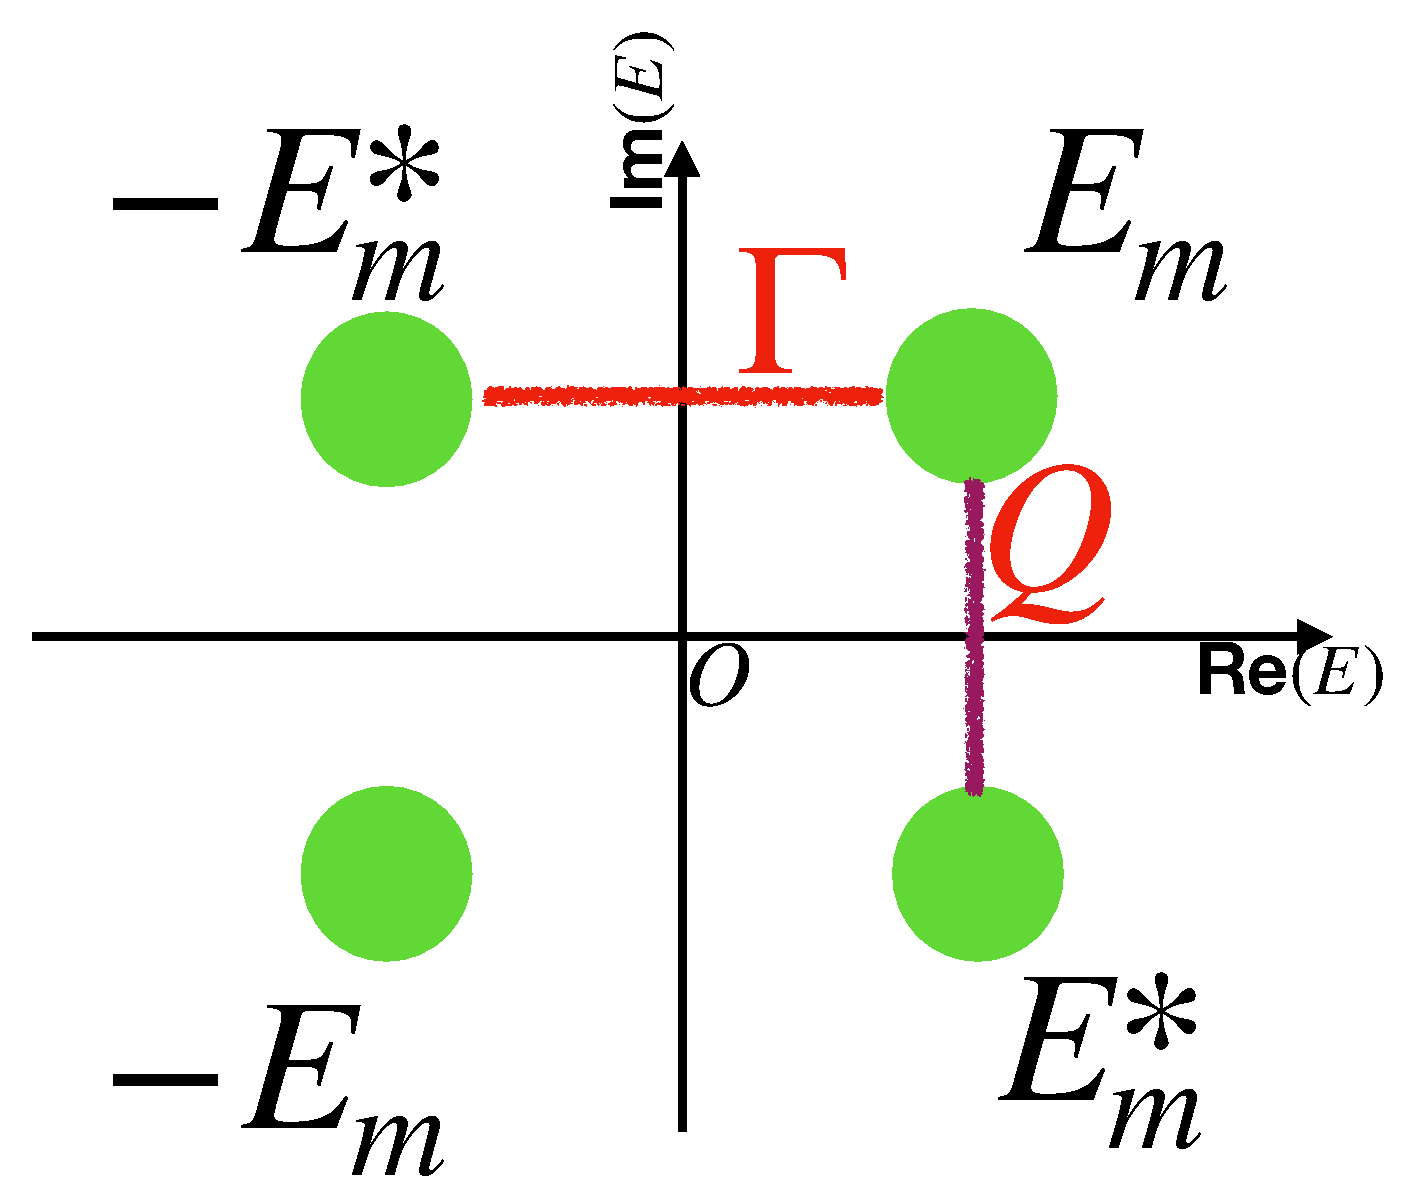
\includegraphics[width=0.7\linewidth]{Figures/topoinsu/sym}
   		\caption{体系的能谱的高对称性和相关的对称性算符。}
   		\label{fig:sym}
   	\end{figure}
   	我们将能谱的结构和对称性算符的关系用图\ref{fig:sym}表示出来。
   	
   	我们可以通过对比体系在两种不同的几何下的能谱,给出体系的相图。体系实部是否简并可以给出有能隙和无能隙的判断,而有限尺寸的边缘激发可以给出来体系的处于绝缘态、量子自旋霍尔态还是导体态。
   	利用波函数判据,我们画出了如下的相图\ref{fig:fig4}。
   	\begin{figure}
   		\centering
   		\includegraphics[width=0.7\linewidth]{Figures/topoinsu/fig4}
   		\caption{非厄米情况下体系的相图。(a,b,c)体系在无穷大格子上的能谱,参数点取在了(d)中的红点。(d)体系的相图,四个相分别是普通绝缘体(NI), 有能隙的量子自旋霍尔态(QSH),无能隙的量子自旋霍尔态(QSH)和无能隙的平庸金属态。途中的两个箭头上的点分别对应图\ref{fig:fig4}里的图(a)-(f)}
   		\label{fig:fig4}
   	\end{figure}
   	
   	\begin{figure}
   		\centering
   		\includegraphics[width=1\linewidth]{Figures/topoinsu/fig5}
   		\caption{体系的波函数。cf\ref{fig:fig4}, (a)-(c)有能隙的QSH到无能隙的QSH到普通导体,(d)-(f)无能隙的QSH到普通的金属到普通的绝缘体。}
   		\label{fig:fig5}
   	\end{figure}
   
   因此,我们发现了全新的、由于非厄米导致的拓扑相。我们如何理解全新的拓扑相,也就是无能隙的二维体系出现了边缘模式?我们可以用图\ref{fig:nonh3}来理解。图\ref{fig:nonh3}(a)和(b)表示了厄米情况的实谱和非厄米情况的虚谱,在能隙关闭和打开的时候,边缘态的不同行为。厄米情况下,由于能隙关闭,体系无能隙的边缘激发和体态发生共振,因此边缘激发消失。非厄米情况下,体系的能谱扩展到复平面上,无能隙的边缘激发可以从虚谱绕过体系的简并点,由于两个波函数的虚部不同,体态和边缘态不发生共振。
\begin{figure}
	\centering
	\includegraphics[width=1\linewidth]{Figures/topoinsu/nonh3}
	\caption{(a)厄米情况下,由于能隙关闭,体系无能隙的边缘激发和体态发生共振,因此边缘激发消失。(b)非厄米情况下,无能隙的边缘激发可以从虚谱绕过体系的简并点,由于两个波函数的虚部不同,体态和边缘态不发生共振。}
	\label{fig:nonh3}
\end{figure}

我们发现我们的系统的确能够很好的用我们上面的图像去描述,如图图\ref{fig:sp32}所展示的那样,体系在圆柱时候的确有类似的边缘模式,在(a)中用红色线标出了,计算能谱之后我们发现它的波函数的确体现出了确定的边缘模式。
\begin{figure}
	\centering
	\includegraphics[width=1\linewidth]{Figures/topoinsu/SP3_2}
	\caption{我们设计的体系的边缘模式,(a)体系在圆柱体几何下的能谱,有两个边缘态绕过了简并点。(b)无穷大体系的能谱,此时能隙已经关闭了(c)(体系在电中性点的波函数。(d)体系的相图,中间的红点是我们选取的参数范围。}
	\label{fig:sp32}
\end{figure}

这个系统中的非厄米拓扑不变量还值得我们去探索\cite{Gong2018topo}。我们把体系写在Chiral算符的表象下$\Gamma = U \sigma_z \otimes I U^\dagger$,由于bi-chiral 对称性,我们有:
\begin{equation}
U H U^{\dagger} =\left( \begin{array}{cc}
iK & q \\ 
q^{\dagger} & iK
\end{array} \right)
\end{equation}
我们于是有$Det H = q q^\dagger - KK$无法再有效的给出同伦不变量$\oint A =\oint \text{tr}(qdq^{-1} - q^{-1}dq)$,这是体系缺少体边对应关系的一个体现\cite{Osterloh2005,leykam2017edge}。进一步的,我们发现基本的对称性($\mathcal{CPT}$)无法给出非厄米体系的分类,总的来说,我们需要一个在K-理论下的38重的分类,其中每一个类的拓扑不变量的确定,还是亟待解决的问题\cite{kawabata2018symmetry,Gong2018topo}。
   \subsection{应用3:超导量子电路测量本征态Kähler流形上的几何学}
   在\ref{sub2}小节中我们讨论了Kähler流形上由希尔伯特空间的内积诱导的黎曼度规和辛2-形式。我们现在指出这两个量都是观测量,可以在超导量子电路中用多种办法测量。接下来我们考虑最简单的2D模型,即希尔伯特空间只依赖两个参数,$(s_1,s_2)$,有时为了方便也混记做$s_\mu,\mu = \{1,2\}$。
   
   \textbf{量子层析办法}是利用超导量子电路层析测量量子态,从而测出每一个点的波函数交叠,随后使用离散化微分为差分的办法直接给出度规和Berry曲率\cite{fukui2005chern}。他的优势在于,理论方法简单,且tomography的方法成熟。但是缺点也是很明显的,由于波函数的维度随着量子系统的尺度指数增加,层析办法是没有可扩展性的,而对于$2\times 2$的模型,$g_{\mu,\nu}, B_{\mu,\nu}$独立的分量是不变的,显然直接测出量子态是用到了非常多的冗余的信息的。
   
   按照第\ref{sub2}介绍的,我们主要是测量以下的几何量,量子度规,其中态$\ket{\phi(s)} = \ket{\phi}$为$H(s)$的本征态,为简便,我们记它为无简并系统的基态:
   \begin{equation}
   g_{\mu,\nu} = \frac{1}{2}(\bracket{\partial_\mu \phi}{\partial_\nu \phi} - \bracket{\partial_\mu \phi}{\phi}\bracket{\phi}{\partial_\nu \phi}) + \mu \leftrightarrow \nu
   \end{equation}
   和2-形式的分量,或者Berry曲率,这里我们不再使用$\sigma$:
   \begin{equation}
   B_{\mu,\nu} = i\partial_\mu(\bracket{\phi}{\partial_\nu \phi} ) - \mu \leftrightarrow \nu
   \end{equation}
   
   这里我们
   注意到二维的反对称张量有特殊的性质,例如我们以测量Berry曲率为例子,将参数空间分解为$N_1 \times N_2$个格点,在每个格点上定义内积$U_\mu$,
   \begin{equation}
   \begin{aligned}
   U_\mu(s) = \bracket{\phi(s + \delta \mu)}{\phi(s)}
   \end{aligned}
   \end{equation}
   定义Wilson loop:
   \begin{equation}
   W(s) = U_1(s)U_2(s + \delta 1)U^*_1(s+\delta 2)U^*_2(s)
   \end{equation}
   可以证明,
   \begin{equation}
   F_{\mu,\nu}(s)dx^\mu dx^\nu \simeq F_{i,j}(s) \delta i \delta j = \arg(W(s))
   \end{equation}
   在进行数值计算的时候,这个方法格外的重要;因为注意到$W(s)$中每一个点的波函数的bra和ket同时出现,因此使用数值对角化的时候他们不具有无关的相位因子。否则:
   \begin{equation}
   \ket{\partial_\mu \phi} \ne \frac{1}{\delta \mu}(\ket{\phi(s + \delta \mu)} - e^{i\phi}\ket{\phi(s)})
   \end{equation}
   直接离散化波函数数值上是错误的。
   
   \textbf{非绝热演化}可以部分的解决上面的问题\cite{kolodrubetz2017geometry}。通过联系黎曼度规和辛2-形式分量和量子态非绝热响应理论得到从可观测量出发测量它们。它的优点在于很多情况下利用系统的对称性和可观测量的特殊形式,只需要测量很少的信息就可以得到量子几何的结构,但是缺点在于,这些对称性和可观测量需要精妙的选取,否则,可观测量的读取依然需要量子层析,这样反而更加麻烦了。
   
   \textbf{周期微扰办法}是近年来讨论较多的办法\cite{palumbo2018revealing,ozawa2018extracting,yu2018experimental}。这种办法的观测量固定为发射率或者量子系统的极化率,给系统施加一个周期的微扰驱动来获得某一个点上的度规和曲率。这样的办法弥补了上面两个办法的缺点,但是依然有不足,那就是需要系统的可控性非常高,这样的办法非常适合NMR这样的量子模拟体系,尤其是在相互作用下,这样的体系给出了新奇的量子几何\cite{Qihaotomography}. 
   
   
   \subsubsection{量子层析办法}
    量子层析办法是指使用超导量子电路中的量子层析技术,在参数空间中测量每一个点的密度矩阵元(固定相位),从而直接得到度规和曲率。这个办法的好处是只需要用到体系基态的波函数;但是缺点也非常明显,那就是没有可扩展性:因为希尔伯特空间的维数是随着体系尺度的增长指数增加的。
    

上面的度规和曲率都是张量的分量,并且是扩展意义下的张量,也就是在规范变换下也是不变的,因此它们似乎是可观测的,但是上面的表达式并不能直接证明它是可以观测的,因为还是涉及到了态矢量。利用态矢量满足$H\ket{\psi} = E_0(s)\ket{\psi}$,我们可以证明,事实上这两个量都和关联函数有关,定义:
\begin{equation}
S_{\mu,\nu}(\omega) = \int_{-\infty}^\infty e^{i\omega t}\avg{\partial_\mu H(t)\partial_\nu H(0)} - \avg{\partial_\mu H(t)}\avg{\partial_\nu H(0)}
\end{equation}
其中$\partial_\mu H(t)$是算符$\partial_\mu H$写在海森堡表象下。
此时,度规写作:
\begin{equation}
g_{\mu,\nu} = \frac{1}{2}\int_0^{\infty} \frac{d\omega}{2\pi \omega^2}(S_{\mu,\nu} + S_{\nu,\mu})
\end{equation}
或者更加简洁的:
\begin{equation}
g_{\mu,\nu} = -\frac{1}{2} \int_0^\infty dt t \avg{\{\partial_\mu H(t), \partial_\nu H(0)\}}
\end{equation}


而Berry曲率是关联函数:
\begin{equation}
B_{\mu,\nu} = -i\int_0^\infty dt t\avg{[\partial_\mu H(t),\partial_\nu H(0)]}
\end{equation}

以上所有的$\avg{\cdots} $都是基态期待值。如果把$F_\mu = -\partial_\mu H$解释为量子广义力,那么度规对应的是广义力的正对易关系,曲率对应的是广义力的反对易关系。

我们以$\avg{[O_\mu(t), O_\nu(0)]} = \avg{[\partial_\mu H(t),\partial_\nu H(0)]} = \avg{U(t)O_\mu(0)U^\dagger(t) O_\nu(0)} - \avg{O_\nu(0)U(t)O_\mu(0)U^\dagger(t) O_\nu(0)}$为例子演示测量的方法,首先将体系制备在$s$处基态$\ket{0}$,然后作用$O_\nu$、演化$U^\dagger(t) = e^{iHt}$、作用$O_\mu$、演化$U(t) = e^{-iHt}$、最后求和基态的保真度,得到第一部分,同理得到第二部分,两者相减得到一个点的数据,在不同时间演化,就可以得到一个参数点的度规和曲率了。

值的提及的是,这样把度规和Berry曲率视作关联函数的做法可以用来识别各种类型的绝缘体\cite{kohn1964theory,resta2006kohn,ozawa2019localization,marrazzo2019local}。这启示我们似乎在多体物理中使用规范理论和几何理论来描述物态的分类更加的自然\cite{wen2004quantum}。

上面的关系涉及极化率以及一个长时间的积分,利用层析办法计算起来有可能较为麻烦而且依赖模型的细节,例如广义力如果是自旋算符等等,就可以直接的测量。但是既然他们都是可观测量,我们可以选取多种办法去测量。下面我们逐一详细描述。
    
   \subsubsection{非绝热演化办法}
   非绝热演化的办法是考虑对体系进行非绝热的演化\cite{kolodrubetz2017geometry,gritsev2012dynamical,roushan2014observation},这个牵引演化的二阶导数为$0$但是一阶导数为有限值,i.e, 是一个非绝热的演化。考虑$s_\mu = s_0 + v_\mu t+ o(v_\mu^2)$体系的广义力的演化可以计算得到:
   \begin{equation}
   \avg{O_\mu}_t = \avg{O_\mu}_0 + B_{\mu,\nu} v_\nu + o(v_\nu^2)
   \end{equation}
   其中$\avg{\cdots}_t = \bra{\phi(t)} \cdots \ket{\phi(t)}$而$\avg{\cdots}_0 = \avg{\cdots}_{t=0}$
   
   这样,通过不同的微小的速度$v_\mu$去驱动系统,通过拟合就能得到$B_{\mu,\nu}$了。
   
   
   如果利用两个方向都驱动,能量的线宽满足:
   \begin{equation}
   \Delta E = \avg{H^2} - \avg{H}^2 = v_\mu g_{\mu,\nu} v_\nu + O(v^3)
   \end{equation}
   通过不同的$v_\mu,v_\nu$和能量期待值,我们就可以测得$g_{\mu,\nu}$了。

   \subsubsection{周期微扰办法}
   周期微扰的办法是利用一个小扰动\cite{palumbo2018revealing,ozawa2018extracting,yu2018experimental}:
   \begin{equation}
   \begin{aligned}
   s_1(t) = s_1(0) + 2(E/\omega)\cos(\omega t)\\
    s_2(t) = s_2(0) \pm 2(E/\omega)\cos(\omega t)\\
   \end{aligned}
   \end{equation}
   我们就有体系的布局数$n_f^\pm(\omega,t) = |\bracket{f}{\psi(t)}|^2$和发射率:
   \begin{equation}
   \Gamma^{\text{int}_\pm} = \frac{1}{t} \int d\omega \sum n_f^\pm(\omega,t)
   \end{equation}
   含时微扰论告诉我们:
   \begin{equation}
    \Gamma^{\text{int}_\pm}  =2\pi E^2 (g_{11}(s^0) \pm 2g_{12}(s^0)+g_{22}(s^0))
   \end{equation}
   
   两个相减得到:
   \begin{equation}
   \Delta \Gamma = 8\pi E^2 g_{22}(s^0)
   \end{equation}
   即对角元。
   
   为了得到非对角元可以只驱动一个参数:
   \begin{equation}
   s_\mu(t) = s_\mu(0) + 2E/\omega \cos(\omega t)
   \end{equation}
   得到:
   \begin{equation}
   \Gamma = 2\pi E^2g_{\mu \mu}(s_\mu^0)
   \end{equation}
   
   \subsubsection{例子:自旋1/2系统以及自旋链系统}
   我们在\ref{subsub2}节中计算了自旋二分之一系统的Berry曲率张量,度规张量也可以简单的计算得到\cite{ozawa2018extracting}:
   \begin{equation}
   g_{\theta\theta} = 1/4, \quad g_{\phi\phi} = \sin^2(\theta)/4,\quad g_{\theta,\phi} = 0
   \end{equation}
   我们可以利用各个方法测量其上的曲率张量和度规张量。
   
   还可以考虑下面的自旋链系统:
   \begin{equation}
   H = \sum_i \bm{B}_i \cdot \bm{\sigma}_i+ \sum_{i} J_{i,i+1} \bm{\sigma}_i\cdot \bm{\sigma}_{i+1} 
   \end{equation}
   其中$\bm{B}_i = (B_x,B_y)$为参数。我们可以数值的得到体系的度规张量和曲率。
   
   我们在图\ref{fig:periodic}中展示了使用非绝热响应(动力学)获得某点的曲率张量,以及使用周期驱动计算度规张量、曲率。我们使用了$TKNN$公式作为理论对比,$TKNN$公式写作:
   \begin{equation}
   \begin{aligned}
   B_{\mu,\nu} = i\sum_{n \ne m} \frac{\bra{n}\partial_\mu H \ket{m}\bra{m}\partial_\nu H \ket{n} - \mu \leftrightarrow \nu}{(E_n - E_m)^2}\\
   g_{\mu,\nu} = i\sum_{n \ne m} \frac{\bra{n}\partial_\mu H \ket{m}\bra{m}\partial_\nu H \ket{n} + \mu \leftrightarrow \nu}{(E_n - E_m)^2}\\
   \end{aligned}
   \end{equation}
   
   
   
\begin{figure}
	\centering
	\includegraphics[width=1\linewidth]{Figures/periodic}
	\caption{(a)周期驱动方法测量自旋1/2系统的量子度规。其中实线为理论预言结果。(b)在自旋1/2系统中验证非绝热微绕理论的正确性范围。显然在$v_1 \ll 1$的时候,非绝热的响应就给出来了体系的Berry曲率。(c)自旋链$N=4$利用(Theoretical),TKNN公式计算的理论结果和(Numerical)利用周期驱动方法的测量结构。(d)自旋链$N = 9,10$利用非绝热微绕测量的自旋链参数空间的陈数随着相互作用强度的变换展现出了量子化的平台。它正对应着某种磁性的霍尔电导。}
	\label{fig:periodic}
\end{figure}
   
   这样的办法被我们称作几何层析方法,使用这种办法可以用来测量复线丛的拓扑不变量陈数:
   \begin{equation}
   C = \frac{1}{2p} \int \mathcal{B}
   \end{equation}
   也可以测量底流形的拓扑不变量欧拉示性数:
\begin{equation}
\chi(S) = \frac{1}{2\pi}[\int_S MdS + \oint_{\partial S}k_gdl]
\end{equation}

除此之外,还可以用我们测得的数据来计算基态量子流形的测地线方程:
\begin{equation}
\ddot{s}^\mu + \Gamma_{\alpha,\beta}^\mu \dot{s}^\alpha \dot{s}^\beta = 0
\end{equation}
可以给出自旋链中量子信息传播的最大速度。
   
   这些工作我们定性的解释到这里,有兴趣的读者可以关注并参考我们将来的(一系列)工作\cite{Qihaotomography}。
   
	\section{结论和展望}
   本文描述了超导量子电路上的量子模拟的新进展,回顾了在几何框架下理解量子物理的数学基础。总结各个章节,
   \begin{enumerate}
   	\item 几何在物理学中扮演了非常重要的地位。一些难以理解的复杂现象,例如经典力学中的绝热不变量、电动力学中的麦克斯韦方程,用几何的方式看起来都相当自然。而量子力学中内蕴的两个结构,一个是辛结构(Berry曲率)和黎曼结构(Fubini-Study度规),用几何理解起来十分的方便。几何中的同伦、同调、上同调理论还可以方便的用来理解拓扑物态。
   	\item 超导量子电路是一种可控性、扩展性都很好的人工量子材料,在其上不仅仅有实现量子计算的可能,还可以用于演示量子光学中的新奇量子相变以及演示量子控制算法,以及模拟各种凝聚态中的新奇现象。
   	\item 超导量子电路量子模拟不仅仅可以用于一般的拓扑物态,还可以研究超出凝聚态框架下的,或者说非厄米下、非阿贝尔规范下的拓扑物态。本文也简述了利用超导量子电路测量卡勒流形上的几何学的办法,这有望启发新的量子控制技术。
   \end{enumerate}
   之后的研究方向可以包括:
   \begin{enumerate}
   	\item 发展实验可行的量子几何层析技术,在此基础上的参数空间的几何测地线方程会扮演什么样的角色?
   	\item 真正的相互作用主宰的多体物理,使用几何的语言应当如何描述?
   	\item 超导量子电路是一种带有自然的耗散的体系。我们可以进一步的研究在耗散下如何稳定物相、耗散和测量如何诱导新奇的多体相?
   \end{enumerate}


	\section{致谢和版权声明}
	这篇毕业论文是我两年以来科研工作的小结。在此论文的完成之际,我必须感谢那些帮助过我关心过我的人,他们的支持是我完成此工作的动力。
	
	
	首先要感谢指导老师胡勇副教授,在整个科研学习中,胡老师对我尽力栽培,从基本物理知识的培养、科研能力的训练,到课题的选取,胡老师都给予了我富有智慧的指导。此外也要感谢物理学院的刘鑫教授和中国科学技术大学的龚明教授,除了知识,从他们那里我还学到了审美和科学态度,令我受益匪浅。还要感谢几位合作老师,包括华南师大薛正远教授等,他们对待科研工作的态度、和对研究课题透彻、智慧的理解,让我从合作中受益良多。
   
    还要感谢物理学院的教职工,本文的实际研究过程超过一年,并且和诸多科大、华南师范、物理所的众多老师和同学讨论过程中,不免会有和平时学院事务冲突的地方,但是学院辅导员刘欢老师、几位教务老师在此之中尽力的协调,感谢他们。特别感谢刘欢老师对我生活和工作中的照料。
	
	我还必须感谢实验室的几位博士生、硕士生学长学姐同学,包括李胜师兄、周孟悦同学、汤秀玉同学。在这样也要感谢在科研中帮助过我、启发过我的热情的朋友们,包括西安交大的郭启淏,西湖大学的唐启承,物理所的潘高培,孙政杭等等。
	
	最后的感谢献给我的父母以及我的妹妹,他们对我的梦想的大力支持是本文的动力之一。
	
	作品中选取了参考文献\cite{GU20171,di2017feynman,Roushan2017a,Roushan2017,owens2018quarter,rechtsman2013strain,rechtsman2013photonic,rechtsman2013topological,hafezi2011robust,hafezi2013imaging,mittal2016measurement,hong2018implementing}的图片,具体的对应已经在图例中标出,它们的版权统一声明如下:
	\begin{enumerate}
		\item 参考文献\cite{di2017feynman}采用Creative Common 3.0 Unported,可以直接使用。 参考文献\cite{GU20171}中的图片,版权归属Elsevier所有,Elsevier和作者(Jia-Qi Cai,蔡家麒)达成了非商用使用协议,\textbf{仅适用于本学位论文},授权号码:4586840831368。
		\item 参考文献\cite{Roushan2017a,rechtsman2013strain,rechtsman2013photonic,hafezi2011robust,hafezi2013imaging,mittal2016measurement}中的图片,版权归属Springer Nature所有,Springer Nature和作者(Jia-Qi Cai,蔡家麒)达成了非商用使用协议,\textbf{仅适用于本学位论文},授权号码:4586530569324, 4586540772000, 4586540933569, 4586541289937, 4586541422687, 4586550065140。
		\item 参考文献\cite{Roushan2017}中的图片,版权归属The American Association
		for the Advancement of Science(AAAS)所有,AAAS和作者(Jia-Qi Cai,蔡家麒)达成了非商用使用协议,\textbf{仅适用于本学位论文},授权号码:4586550196697。
		\item 参考文献\cite{owens2018quarter,hong2018implementing,rechtsman2013topological}中的图片,版权归属American Physical Society(APS)所有,APS和作者(Jia-Qi Cai,蔡家麒)达成了非商用使用协议,\textbf{仅适用于本学位论文},授权号码:RNP/19/MAY/014779, RNP/19/MAY/014777, RNP/19/MAY/014780。
	\end{enumerate}
	同时也感谢Elsevier, IOPscience, APS, Springer Nature, AAAS对本文一些插图的授权使用。
	
	此外,本工作还涵盖了已经发行了预印本\cite{sun2018out,cai2018non}、或未来有可能发表的图片\cite{Qihaotomography},它们的版权目前由作者享有,但引用应当视最后出处决定。
	\section{本科发表的工作}
	\begin{itemize}
		\item \label{nonadia}Implementing universal nonadiabatic holonomic quantum gates with transmons,
		Zhuo-Ping Hong\footnote{这些作者为共同第一作者 \label{equal}}, Bao-Jie Liu\textsuperscript{\ref{equal}}, \textbf{Jia-Qi Cai}\textsuperscript{\ref{equal}}, Xin-Ding Zhang, Yong Hu, Z. D. Wang, Zheng-Yuan Xue \href{https://arxiv.org/abs/1710.03141}{arXiv:1710.03141},  \href{https://link.aps.org/doi/10.1103/PhysRevA.97.022332}{Phys. Rev. A, {\bf 97}, 022332} 
		\item \label{OTOC}
		Out-of-time-order correlation functions as indicators of quantum phase transitions in the Rabi and Dicke model. Zheng-Hang Sun\textsuperscript{\ref{equal}}, \textbf{Jia-Qi Cai}\textsuperscript{\ref{equal}}, Qi-Cheng Tang, Yong Hu, Heng Fan,  \href{https://arxiv.org/abs/1811.11191}{arXiv:1811.11191}
		\item \label{SOC} Non-Hermitian topological microwave photonics with synthetic non-Abelian gauges. \textbf{Jia-Qi Cai}, Zheng-Yuan Xue, Ming Gong, Guang-Can Guo, Yong Hu \href{https://arxiv.org/abs/1812.02610}{arXiv:1812.02610}
	\end{itemize}
	\nocite{*}
	\bibliography{reference.bib}
	
	\begin{appendices}
		\section{微分形式\label{appendix: Differential}}
		我们将矢量(逆变矢量,切矢量)定义为标量函数的某种一阶微分算符。简单的来说,我们考虑 $\mathbf{R}^n$ 上某点和原点构成的射线 $\mathbf{r}$ ,和这个点上的一组坐标, $u^i,i \in {1,2,...,n}$ ,那么这一点任何一个矢量 $\mathbf{v}$ 都可以用 $\hat{\partial}_i = {\partial \mathbf{r} \over {\partial u^i}}$ 展开: $\mathbf{v} = \Sigma_i v^i \hat \partial_i$。这样我们就可以继续定义矢量对一个标量函数的作用
		\begin{equation}
		 \mathbf{v} [f] = (\Sigma_i v^i\hat \partial_i )[f] \equiv \Sigma_i ({\partial f \over {\partial u^i}})v^i
		\end{equation}
	即,矢量对标量函数的作用就是将标量函数“沿着”矢量微分。
		
		我们来考虑对偶矢量(协变矢量,1-形式)。线性代数中对偶向量空间$ V^*$ 是一类线性泛函 $\alpha: V \to R, \alpha[\mathbf{v}]=  \Sigma_i a_i v^i$ , 函数的微分 $(df)_i \equiv {\partial f \over{\partial u^i}}$ 那么 $df$ 对矢量的作用就是: $df[\mathbf{v}] = \Sigma_i{\partial f \over{\partial u^i}} v^i  \equiv \mathbf{v}[f]$ . 我们接下来想要去寻找对偶矢量的一组基,记作 $\hat \partial^i_*$ ,那么按照定义,应当满足 $\hat \partial^i_*(\partial_j) = \delta_j^i$ 那么他作用在矢量 $\mathbf{v}$ 上的结果,经过一番计算,是$\hat \partial^i_* \mathbf{v} = v^i$ ,我们又知道, $\mathbf{v}[u^i] = \Sigma_j \delta_j^i v^j=du^i[\mathbf{v}]=v^i$ ,所以我们不妨就这样来书写:$ \hat \partial^i_* = du^i$ ,这样写的好处在于: $df[\mathbf{v}] = \Sigma_i{\partial f\over{\partial u^i}} v^i=\Sigma_i{\partial f\over{\partial u^i}} du^i[\mathbf{v}]$ ,因此 $df =\Sigma_i{\partial f\over{\partial u^i}} du^i$ .有了基,我们就可以将对偶矢量 $\alpha$ 按照基展开了: $\alpha = \Sigma_i \alpha_i du^i$ 。对比上一个式子,可能有某些$ \alpha = df$ ,但是这并不必要成立。
		
		接下来我们将默认使用爱因斯坦求和约定,i.e,对相同的上指标和下指标自动求和. 按照这个规则,一个逆变矢量作用在矢量上,自动给出 $\alpha[\mathbf{v}] = \alpha_i v^i$ , 不妨也定义矢量对协变矢量的作用 $\mathbf{v}[\alpha] = \alpha[\mathbf{v}] = a_i v^i$ .
		请自行验证,在坐标变换下 $u \to u'$ ,逆变矢量按照 $v'^j = \frac{\partial u'^j}{\partial u^i} v^i$ 而协变矢量按照 $\alpha'_j = a_i \frac{\partial u^i}{\partial u'^j}$,而 $a_i v^i$ 是一个不变量。
		
		我们接下来考虑定义张量积,来诱导出更多的结构。考虑两个协变矢量的张量积定义为矢量的有序数对$ (\mathbf{w},\mathbf{v})$ 的线性函数, $\alpha \otimes \beta [(\mathbf{w},\mathbf{v})] = \alpha(\mathbf{w}) \beta(\mathbf{v})$ ,以此类推,注意 $du^i \otimes du^j [(\mathbf{w},\mathbf{v})] = w^i v^j$ ,同样的 $\hat \partial_i \otimes \hat \partial_j [(\alpha, \beta)] = a_i b_j$ ,我们可以利用这些性质构造协变、逆变和混变的张量,例如二阶协变张量, $T = a_{ij} du^i \otimes du^j = a_{ij} du^idu^j$ ,之后,我们会忽略对偶矢量的直积符号。三阶混变张量:$ A = \hat \partial_i \otimes \hat \partial_j A^{ij}_k \otimes du^k $等等。
		请自行验证,在坐标变换下,张量的逆变指标按照逆变规则变化,协变指标按照协变规则变化。
		
		我们接下来来讨论两类特殊的二阶张量,一个是度规张量,一个是线性变换。
		一个线性变换是一个二阶混变张量, $U = \hat \partial_i P^i_j  \otimes du^j $,它可以将一个矢量映射到一个矢量。自行证明 $P(\mathbf{v}) = P^i_j v^j \hat \partial_i$ 是一个矢量。
		要讨论度规就要默认我们的空间里又配备上了(赝)内积结构 $\inp{ }{ }$ 了,考虑 $\mathbf{R}^n$ 上的不变长度例如 $ds^2 = \Sigma_k dx^k dx^k$ ,在曲线坐标下,他就是 $ds^2 = \Sigma_{i,j} g_{i,j}du^idu^j = g_{i,j}du^i du^j$ , 其中我们利用了 $dx^k = \frac{\partial x^k}{\partial u^i} du^i $,其中 $g_{i,j} = \Sigma_k \frac{\partial x^k}{\partial u^i} \frac{\partial x^k}{\partial u^j} = \inp{\frac{\partial\mathbf{r}}{\partial u^i}}{\frac{\partial\mathbf{r}}{\partial u^j}} = \inp{\hat \partial_i}{ \hat \partial_j}$,因而度规张量 $g_{i,j}$ 是一个对称张量,请自行验证,这样定义的度规张量却是满足张量的变换规律。当然如果反着来定义,先钦定一个度规张量,然后定义一个内积结构,这个内积结构不妨就写作 $\inp{\mathbf{v}}{\mathbf{w}} = ds^2[\mathbf{v},\mathbf{w}]=g_{ij}v^i w^j$ . 
		有了度规张量,我们相当于定义了矢量对矢量的运算,也就联系了矢量如何对应上对偶矢量,i.e利用 $v[\mathbf{u}] = \inp{\mathbf{v}}{\mathbf{u}}$ ,我们就有 $v_j w^k = v^k g_{kj} w^j \to v_j = v^k g_{kj}$ . 将上式子视为变换,接下来,我们可以定义这个变换的逆变换 $v^k = g^{kj}v_j$ ,可以通过定义证明 $(g^{jk} \hat \partial_j \otimes \hat \partial_k)$ 这个张量是一个二阶逆变张量, 且由于对偶矢量基作用在矢量基上的性质, $g^i_k \equiv g^{ij} g_{jk}  = \delta^i_k$ .有了度规张量我们也能看梯度矢量了,我们想构造 $(\nabla f)^i \equiv g^{ij} \frac{\partial f}{\partial u^j}$ ,进而几步思考我们就可以得到 $df(\mathbf{w}) =  \inp{\nabla f}{ \mathbf{w}} $.,这样,我们就在度规张量的帮助下定义了带度规的grad. 
		
		讨论完了张量运算,我们考虑一类特殊的张量,$n$-形式,它们在几何上有更加重要的地位。
		我们首先定义外积,考虑两个对偶矢量,或者1-形式, $\alpha^1, \beta^1$ ,他们的外积运算定义为 $\alpha^1 \wedge \beta^1 \equiv \alpha^1 \otimes \beta^1 - \beta^1 \otimes \alpha^1 $。这样的一个反对称协变二阶张量叫做(外)2-形式。更加一般的2-形式可以写作$ \beta^2 = b_{ij} du^i \wedge du^j, b_{ij} = - b_{ji}$ 。由此推广到反对称协变p阶张量就是p-形式,这里的反对称是指的,以p个矢量为宗量的p-形式,对每一个位置的交换,值都会给出一个负号。
		我们以 $\mathbf{R}^3$ 作为例子:按照定义,对于不同的 $j,k$ 有$dx^j \wedge dx^k = - dx^k \wedge dx^j , dx^k\wedge dx^k = 0 (\text{no summation}) $.
		$\mathbf{R}^3$中一般的2-形式可以写作$ \beta ^2 = b_{23} dx^2 \wedge dx^3 + b_{31} dx^3 \wedge dx^1 + b_{12} dx^1 \wedge dx^2 $
		3-形式可以写作 $\gamma^3 = b_{123} dx^1\wedge dx^2 \wedge dx^3$ 
		我们可以用行列式的行列交换性质轻松的定义出$p$-形式对矢量的左右.
		我们可以补充定义$p$-形式和$q$-形式之间的外积,运算规则就是使得外积拥有结合律,并依次展开,例如:
		\begin{equation}
		\begin{aligned} \omega^1 \wedge \alpha^1 &= (\omega_i dx^i)\wedge(a_j dx^j) \\ &=(\omega_1 dx^1)\wedge (a_2 dx^2)+\cdots (\omega_2 dx^2)\wedge(a_1 dx^1) + \cdots \\  &=(\omega_2 a_3 - \omega_3 a_2)dx^2\wedge dx^3 + (\omega_3 a_1- \omega_1 a_3)dx^3 \wedge dx^1 \\ &+ (\omega_1 a_2 - \omega_2 a_1)dx^1 \wedge dx^2 \end{aligned} 
		\end{equation}
		再来看一个1-形式和2-形式的作用:
		\begin{equation}
				\begin{aligned} \alpha^1 \wedge \beta^2 &= (a_i dx^i) \wedge (b_{23} dx^2 \wedge dx^3\\ &+b_{31}dx^3 \wedge dx^1 + b_{12}dx^1 \wedge dx^2)\\ &=(a_1 b_{23} + a_2 b_{31} + a_3 b_{12})dx^1\wedge dx^2\wedge dx^3\\ &=(a_i b_i)dx^1\wedge dx^2\wedge dx^3 \end{aligned} 
		\end{equation}
		其中 $b_1 = b_{23}, b_2 = b_{31},b_3 = b_{12} $
		读者可以自行使用行列式证明,$p$-形式和$q$-形式在外积前后交换,满足规则 $\alpha^p \wedge \beta^q = (-1)^{pq} \beta^q \wedge \alpha^p $
		
		我们知道,$ T_b^a = \frac{\partial v^a}{\partial u^b}$ ,即使是 $v^a$ 是矢量分量, $T^a_b$ 也不一定是一个张量的分量. 定义外微分,就是要定义一个$p$-形式到$p+1$-形式的运算,我们作出如下定义:
		\begin{equation}
		d[adu^1\wedge du^2 \cdots \wedge du^k] = da \wedge du^1\wedge du^2 \cdots \wedge du^k =\Sigma_r (\frac{\partial a}{\partial u^r})du^r\wedge du^1\wedge du^2 \cdots \wedge du^k 
		\end{equation}
		这个定义在 $\mathbf{R}^3$ 立刻可以得到我们关于多变量微积分的一些认识,例如:
		\begin{equation}
		df = \frac{\partial f}{\partial x^i} dx^i  , d\alpha^1 = d(a_i dx^i) = \Sigma_k(P_{ijk}  \frac{\partial a_i}{\partial x^j} dx^i dx^j) , d\beta^2 = \frac{\partial b_i}{\partial x^i} dx^1 \wedge dx^2 \wedge dx^3 
		\end{equation}
		显然有 $df \Leftrightarrow \text{grad}f (\mathbf{dx}), d\alpha^1 \Leftrightarrow (\text{curl } \mathbf{a}) \cdot \mathbf{dA}, d\beta^2 \Leftrightarrow  \text{div } \mathbf{B} \cdot dV$  ,grad的定义已经给出,我们后面会给出curl和div的定义.
		一个有用的公式是 \begin{equation}
		d(\alpha^p \wedge \beta^q) = d\alpha \wedge d\beta + (-1)^p \alpha \wedge d\beta 
		\end{equation}
		
		考虑映射 $F: \mathbf{R} ^k \to \mathbf{R}^n $,其上两个曲线坐标分别是 $\{ u^1, \cdots ,u^k\},\{ x^1, \cdots ,x^n\}$ ,因此 $F$ 可以用$n$个函数 $x^i = F^i(u) \equiv x^i(u)$ 描述. 有了这个映射关系,在此基础上,我们来定义推前和拉回.
		现在来考虑推前. 考虑 $u_0 \in \mathbf{R}^k$ 上的一个矢量 $\mathbf{v}_0$ ,这个矢量一定都与一个参数曲线的速度对应,例如 $u = u(t) , u(0) = u_0$ 在$ t = 0$ 处的速度:$ \mathbf{v}_0 = [\frac{du}{dt}]_0$ .基于此,我们可以定义矢量的在 $x_0 = F(u_0) \in \mathbf{R}^n$ 的推前,利用所谓的“$F$ 的微分”,$ F_*$ ,他作用在矢量 $\mathbf{v}_0$ 就给出了$ t = 0$ 时候 $x(t) = x(u(t))$ 的速度 $F_*[\mathbf{v}_0]$ ,用表达式就是:
\begin{equation}
		[F_*\mathbf{v}_0]^i = [\frac{dx^i(u(t))}{dt}]_0 = [\frac{\partial x^i}{\partial u^r}]_{u(0)} [\frac{du^r}{dt}]_0=[\frac{\partial x^i}{\partial u^r}]_{u(0)}  \mathbf{v}_0^r
\end{equation}
因此,$ [F_* \mathbf{v}]^i = v^r\frac{\partial x^i}{\partial u^r}$
		不妨验证,这样定义的推前作用在矢量基上就是链式法则:
		$F_*\hat\partial_r = \frac{\partial x^i}{\partial u^r} \hat \partial _i $。
		对于一个定义在 $x \in \mathbf{R}^n$ 点上的$p$-形式 $\alpha$ , 我们定义 $\alpha$ 的拉回 $F^*[\alpha]$  是一个定义在原像空间 $u \in F^{-1} (x)$ 的$p$-形式,满足:
		$F^* \alpha [\mathbf{v},\cdots,\mathbf{w}] \equiv \alpha[F_*\mathbf{v},\cdots, F_*\mathbf{w}] $。
		不妨验证,这样的定义的拉回作用在对偶矢量基上就是链式法则:
		$F^*dx^i = \frac{\partial x^i}{\partial u^s} du^s$ 。
		上面拉回即使对于不是外形式的协变张量也能够定义.
		拉回有一些重要的关系,例如 $F^*[\alpha^p \wedge \alpha^q] = F^*\alpha \wedge F^* \beta$ 和$ dF^* \alpha = F^* d\alpha$ .
		利用拉回的上面的性质,不难验证:
		$F^*[dx^i \wedge \cdots \wedge dx^j] = \Sigma_{a<\cdots < r} [\frac{\partial(x^i,\cdots,x^j)}{\partial (u^a,\cdots u^u)}] du^a\wedge \cdots \wedge du^r $
		
		我们现在可以开始想办法定义$p$-形式的积分了. 
		我们先考虑一个特例,看看$ F: [a,b] \subset \mathbf{R}^1 \to C \subset \mathbf{R}^3$ ,以及 $\mathbf{R}^3$ 上的一个1-形式 $\alpha = a_i(x)dx^i$ 
		定义$ \int_C \alpha = \int_C a_i dx^i \equiv \int_a^b F^*\alpha = \int_a^b a_i(x(s))\frac{dx^i}{ds} ds$ 这样就以对应上我们以及学过的积分定理了以对应上我们以及学过的积分定理了 .
		有了上面的直觉我们定义面积分,甚至定义任意流形上的积分都是很简单的.
		例如考虑 $S \subset \mathbf{R}^2 \to V \subset \mathbf{R}^3 , x^i = x^i(s^1,s^2) $,以及 $\mathbf{R}^3$ 上的一个2-形式 $\beta = b_1 dx^2 dx^3 + b_2 dx^3 dx^1 + b_3 dx^1 dx^2 $
		定义$ \int_V \beta = \int_S F^*\beta$ ,这个时候上面的拉回公式就起作用了,考虑其中的一个分量:
		\begin{equation}
		\int_S F^*[b_1 dx^2 dx^3] = \int_S b_1(x(s))[(\frac{\partial x^2}{\partial s ^a})ds^a \wedge (\frac{\partial x^3}{\partial s ^b})ds^b] =\int_S b_1(x(s)) [\frac{\partial(x^2,x^3)}{\partial(s^1,s^2)}] ds^1ds^2   
		\end{equation}
		因此:\begin{equation}
		 \int_V \beta = \int_S\{ b_1(x(s)) [\frac{\partial(x^2,x^3)}{\partial(s^1,s^2)}] + b_3(x(s)) [\frac{\partial(x^1,x^2)}{\partial(s^1,s^2)}] + b_2(x(s)) [\frac{\partial(x^3,x^1)}{\partial(s^1,s^2)}] \} ds^1 ds^2
		\end{equation}
		以后推广到微分流形上,也有 $\int_\sigma \omega = \int_D F^*\omega $,$ \sigma$ 是一个奇异$p$-多面体, $D$是 $\mathbf{R}^k$ 上的一个突-$k$多面体.
		一个重要的、联系外微分和如上定义的积分的重要公式是斯托克斯公式,也叫做牛顿-莱布尼茨-高斯-格林-奥斯特-斯托克斯-庞加莱公式,通常也被认为是世界上最美的公式:
		$\int_V \beta^{p-1} = \int_{\partial V} d\beta^{p-1}$,其中, $V$ 是一个$p$维的曲面,有一个 $(p-1)$ 维可定向的边界 $\partial V$ .
		
		们现在来用新语言来描述平直空间 $\mathcal{R}^3$ 的电动力学, 其中时间变量$t$为一个参数. 
		电场强度$E$是和力以及功直接相关的一个量,由于涉及线积分,因此我们考虑他对应的一个1-形式:$ \mathcal{E}^1 = E_i dx^i$  , 功就由它的积分给出 $\mathcal{w} = q\int_C \mathcal{E}^1$ . 
		电场$D$是进入高斯定理和高斯定理有关的一个量,由于涉及面积分,因此我们考虑他对应的一个2-形式:$ \mathcal{D}^2 = E_1 dx^2 dx^3 + E_2 dx^3 dx^1 + E_3 dx^1 dx^2 $,他的积分就给出 $\int_{\partial V}\mathcal{D} = \int_V d\mathcal{D} = 4\pi Q = 4\pi \int_V \rho \text{ vol}^3 \to d\mathcal{D}  = 4\pi \rho \text{ vol}^3$ ,$ \rho$ 是一个标量.
		磁场强度$B$是电场强度的线积分有关的一个量,按照法拉第定律,电场强度的微分给出了磁场强度,因此对应一个二形式: $\mathcal{B}^2 = B_1 dx^2dx^3 + B_2 dx^3 dx^1 + B_3 dx^1dx^2$ ,磁场本身满足散度定律: $d \mathcal{B} = 0$ 并以法拉第定律和 $\mathcal{E}$ 联系:$ d \mathcal{E} = - \partial_t \mathcal{B} $
		磁场$H$是一个和电流密度的变换有关的,电流密度的面积分和电荷标量的速率有关因而是一个2-形式$ \mathcal{J}^2$ , 因此磁场对应的是1-形式: $\mathcal{H}^1= B_i dx^i$ ,由安培-麦克斯韦定律我们知道:
		$\int_{\partial V} \mathcal{H} = 4\pi \int_V \mathcal{J} + \frac{d}{dt} \int_V \mathcal{D} $因此利用斯托克斯定理: $d \mathcal{H} = 4\pi \mathcal{J} + \frac{d}{dt} \mathcal{D}$ .
		在没有定义任意流形的微分形式之前,我们最远也就是走到这里了. 我们看到电动力学还是非常的复杂。但是随后在进入了民科夫斯基空间上定义微分形式之后,电动力学会变得非常简单和自然。
		
		
		我们还缺少一种运算。通过函数作用,我们有1-形式和矢量之间的内积,我们还通过通过度规张量定义了两个矢量之间或者两个1-形式之间的内积. 但是在电动力学中,磁场 $H$ 是用一个2-形式表示,而电场、力都是1-形式,而洛伦兹公式 $\mathcal{F} = q(\mathcal{E}^1 + ? \mathcal{B}^2) $,问号处是速度矢量的一个函数,作用在磁场2-形式 $\mathcal{B}$ 上。同时,在麦克斯韦理论中$E$和$D$,$H$和$B$之间是有联系的。因此,将一个矢量作用在一个 $p$ -形式上得到一个$p-1$形式就是为我们需要的, 他有着内积的推广的意义.
		我们定义 $\mathbf{v}$ 和$p$-形式 $\beta$ 的内积$ i_\mathbf{v} \beta$ 为一个$p-1$形式,他对于矢量对 $(\mathbf{w}_1,\cdots , \mathbf{w}_{p-1})$ 的作用为:
		$i_{\mathbf{v}}\beta [\mathbf{w}_1,\cdots , \mathbf{w}_{p-1}] \equiv \beta[\mathbf{v},\mathbf{w}_1,\cdots , \mathbf{w}_{p-1}] $
		很显然,一个矢量对一个1-形式会得到标量0-形式: $i_{\mathbf{v}} \alpha = \alpha[\mathbf{v}] = a_i v^i$ 具有扩展的内积定义.
		容易验证 $i_{\mathbf{v}} (\alpha^1 \wedge \beta^1)[\mathbf{w}] = \alpha^1 \wedge \beta^1(\mathbf{v},\mathbf{w}) = [(i_{\mathbf{v}}\alpha)\beta-(i_{\mathbf{v}}\beta)\alpha][\mathbf{w}] $, 不难推广:
		$i_{\mathbf{v}} (\alpha^p \wedge \beta^q) = [i_{\mathbf{v}}\alpha^p] \wedge \beta^q + (-1)^p \alpha^p \wedge i_{\mathbf{v}} \beta^q$
		我们现在可以写出洛伦兹力公式了: $\mathcal{F} = q(\mathcal{E} - i_{\mathbf{v}}\mathcal{B})$ ,但是为什么 $i_{\mathbf{v}}\mathcal{B} $是$ \mathbf{R}^3$ 中外积的推广呢?且看下节体形式。
		
		我们还没能列入一些关键的事情,例如我们如何理解通常微积分中对一个0-形式的体积分$ \int_V f \text{ vol}$ ?特殊的,当 $f = 1$ 我们得到的是区域 $V \subset \mathbf{R}^k$ 的体积,很显然, $\text{vol}$ 应当是一个$k$-形式. 体积是一个度量性质,很显然要和度规有关了. 我们如果默认 $\text{vol}^2 = dxdy$ ,在极坐标就有 $\text{vol}^2 = rdr\wedge d\theta$ ,我们定义:
		$\text{vol}^n = \sqrt{|det(g)|} dx^1 \wedge\cdots\wedge dx^n$ ,就可以了。
		另外我们没能列入的,例如面积形式,无非是用矢量 $\mathbf{n}$ 和体形式内积得到:
		$\text{Area}^2 = i_{\mathbf{n}} \text{vol}^3$ 并以此类推。
		有了体形式,我们还可以定义对矢量场的散度:(区别于对1-形式)
		$\text{div } \mathbf{v} \text{ vol}^n \equiv d(i_{\mathbf{v}} \text{vol}^n) = (1/\sqrt{|det(g)|}) \partial_{x^i} \sqrt{|det(g)|}v^i \text{ vol}^n$ 
		另外,注意到在 $\mathbf{R}^3$ 中有一类非常特殊的运算,那就是矢量的叉积$\mathbf{a} \times \mathbf{c}$,而我们已经知道了,2-形式 $\alpha^1 \wedge \beta^1 $和 $\mathbf{a} \times \mathbf{c} $有关,如何能够从$\mathbf{a} \times \mathbf{c}$定义一个1-形式呢?
		一个办法是定义1-形式 $\delta^1 = (\mathbf{a}\times\mathbf{b})_*  = -i_\mathbf{a}[i_{\mathbf{b}} \text{ vol}^3]$ 
		回到洛伦兹力公式为什么可以写作$\mathcal{F} = q(\mathcal{E} - i_{\mathcal{v}}\mathcal{B})$的问题,我们只需定义 $\mathcal{B}=i_{\mathbf{b}}\text{ vol}^3,b^i=b_i/\sqrt{det(g)} $就会得到自洽的叉乘结果了.
		
		我们已经提到了div和grad,下面我们想要去定义curl,在欧空间中我们去定义Hodge算符$*$:
		$\alpha^p \wedge *\beta^p = <\alpha,\beta> \text{vol}^n $,
		即$*$能把一个$p$-形式映射到$n-p$形式上. 我们考虑在 $\mathbf{R}^3$ 上的直角坐标系演示如何拿到hodge算符的具体表达式:
		很显然$ *dx = dydz, *dy=dzdx,*dz=dxdy$ ,以及 $*1 = dxdydz, *dxdydz=1$ 
		对于一形式 $\alpha = a_1dx+a_2dy+a_3dz,\beta = b_1 dx+b_2dy+b_3dz$ ,
		$*(\alpha \wedge \beta) = (\mathbf{a} \times \mathbf{b})_*$ 刚好给出了叉积!而 $*d*\alpha = \text{div } \mathbf{a}$ 给出了div.我们不妨就将它定义成对对1-形式的div(而非对应的矢量)。
		考虑1-形式 $\omega $,$d\omega$ 成为一个2-形式,而 $*d\omega$ 返回了一个1形式,并带有微分算符,不难验证,它正是作为curl的推广,新定义的curl作用一个1-形式返回一个1-形式.
		我们可以通过矢量内积将$p$形式变换到$p-1$形式,并和度规无关。而现在有了霍奇算符$*$,我们又可以定义另外一种重要的、和度规有关的算符,余微分,将$p$形式变换到$p-1$形式:
		$d^\dagger \alpha^p = (-1)^{n(p+1) +1} *d*\alpha^p$ 
		在 $\mathbf{R}^3$ 中不难验证 $\Delta = -dd^\dagger - d^\dagger d = \nabla^2 $.
		总结一下,有了余微分和hodge算符这两个用体形式定义出来的算符,我们有 $\text{grad }f^0 = df, \text{curl } \alpha^1 = *d\alpha, \text{div } \alpha^1 = *d*\alpha =-d^\dagger \alpha$, 
		利用这些关系,我们可以计算一系列复杂的算符组合,例如
		$\text{curl }\text{curl } \alpha=*d*d\alpha = d^\dagger d\alpha= -dd^\dagger \alpha -\Delta \alpha = d(*d*)A -\Delta \alpha = \text{grad} \text{ div} \alpha - \Delta \alpha   $
		其对应的矢量运算(利用度规交换过来)法则正是:$
		\nabla \times (\nabla \times \mathbf{a}) = \nabla(\nabla \cdot \mathbf{a}) - \nabla^2 \mathbf{a}$ (为了区别于对偶矢量不是用grad div curl)
		
		
		\section{基本群、高维同伦群和拓扑不变量\label{appendix: homology}}
		
		\textit{拓扑空间闭道路的等价类。}考察$R^2$上两个区域$X_1$和$X_2$,其中$X_1$有洞而$X_2$无洞,而在$X_1$上,由于没有洞,因此任何一个封闭的道路(闭道路)都可以连续的收缩到一点,因此过固定点的闭道路都能相互连续的收缩形变,因此构成一个等价类。但是对于$X_2$区域,存在两种不同的闭道路,第一类能够连续的收缩到一点,而第二类不能,根据这样的性质,他们可以分成两种等价类,或者说同伦类。为了研究其上的结构,我们考虑补充定义乘法$*$,考虑顺时针的闭道路的等价类为$\gamma$正元素,而逆时针为$\gamma^{-1}$逆元素,因而其上有自然的乘法$\gamma = \alpha * \beta$表示先绕着$\alpha$道路走再绕着$\beta$道路走。按照上面定义的等价关系,我们知道这个乘法和元素满足群的定义。这样定义出来的群就是基本群。
		
		上面的解释,给我们了一个直觉上的体验,即拓扑空间中闭道路的等价类可以描述空间上洞的性质。我们下面补充更加精确一些的定义。
		
		\textit{道路连通:} 考虑$I = [0,1]$是$R$上的一个单位闭区间,$X$为一个拓扑空间,连续映射$\alpha: I \to X$使得$\alpha(0) = x_0, \alpha(1) = x_1$,我们把$x_0$叫做\textbf{起点},$x_1$叫做\textbf{终点},而$\alpha(t)$本身叫做\textbf{道路}。
		
		\textit{评论:}按照上面群的精神,我们还可以定义“逆时针”的逆道路,考虑下面的定义:
		
		\textit{逆道路:}考虑$\alpha(t): I\to X$是$x_0$到$x_1$的道路,定义\textbf{逆道路}为$\alpha^{-1}(t) =  \equiv \alpha(1-t)$是$x_1$到$x_0$的道路。
		
		\textit{道路连通:}如果拓扑空间$X$上的任意两点$x_0, x_1$都存在$x_0$到$x_1$上的一条道路$\alpha$,则说这个拓扑空间是\textbf{道路连通}的。
		
		\textit{评论:}道路连通的拓扑空间强于\textbf{连通性}。即道路连通的拓扑空间一定是连通的,但是反之不然。
		
		\textit{圈:}拓扑空间$X$中,满足$\alpha(0) = \alpha(1) = x_0$的道路$\alpha$叫做\textbf{闭道路},或者\textbf{圈},$x(0)$称作基点。如果$\gamma(t) = c_0$为常数,这样的$\gamma$满足圈的定义,定义为起点\textbf{常值圈}。
		
		\textit{评论:}现在我们有了闭道路的完整的描述。我们接下来来定义刚刚提到的作为群乘法的运算,即圈之间的乘法。
		
		\textit{圈之间的乘法运算:} 
		\begin{enumerate}
			\item 考虑过基点$x_0$的圈$\alpha,\beta$定义它们的乘积$\gamma = \alpha * \beta$也是过$x_0$的圈,定义为:
			\begin{equation}
			\gamma(t)  = \begin{cases}
			\alpha(2t) &0\le t \le {1\over 2} \\
			\beta(2t-1)  &{1\over 2} \le t \le 1
			\end{cases}
			\end{equation}
			这个定义的意义就是先沿着$\alpha$转动然后沿着$\beta$转。
			\item 逆圈被定义为圈对应的逆道路,即$\alpha^{-1}(t) = \alpha(1-t)$
		\end{enumerate}
		
		\textit{同伦:}考虑过基点$x_0$的$\alpha, \beta$定义它们之间的\textbf{同伦},若果存在连续映射$H: I \times I = [0,1] \times [0,1] \to X$,满足:
		\begin{equation}
		\begin{aligned}
		H(t,0) &= \alpha(t), 0\le t\le 1\\
		H(t,1) &= \beta(t),0\le t \le 1\\
		H(0,s)&=H(1,s) = x_0, 0\le s\le 1
		\end{aligned}
		\end{equation}
		则称映射$H$是$\beta$和$\alpha$之间的同伦。
		
		\textit{评论:}这样的$H$诱导出来的等价关系$\alpha \simeq \beta$可以简单的证明具有自反律$\alpha \simeq \alpha$、对称律$\alpha \simeq \beta \to \beta \simeq \alpha$、传递律$\alpha \simeq \beta, \beta\simeq\gamma \to \alpha \simeq \gamma$,同时还容易证明有关系$\alpha \simeq \beta \to \alpha^{-1} \simeq \beta^{-1}$和$\alpha_1 \simeq \alpha_2, \beta_1 \simeq \beta_2 \to \alpha_1 *\beta_1 \simeq \alpha_2 \beta_2$。诱导的划分给出\textbf{同伦类},即$\beta\simeq\alpha$的全体$\beta$,其中$\alpha$为代表元素。
		
		\textit{基本群:} 考虑$[\alpha]$是代表元素为$\alpha$的同伦类,他们构成的$X$中过$x_0$点的圈的前提同伦类的集合记做$\pi_1(X,x_0)$,对于$[\alpha], [\beta]$构成的同伦类,$[\alpha] \circ [\beta] \equiv [\alpha * \beta]$,容易证明这样定义的乘法满足结合律。因此,$\pi_1(X,x_0)$上述定义的乘法运算下成群,补充单位元的定义为过$x_0$的常值圈构成的同伦类,而$[\alpha]$的逆元为$[\alpha^{-1}]$。群$\pi_1{X,x_0}$称为拓扑空间$X$在$x_0$处的\textbf{第一同伦群}或者\textbf{基本群}。
		
		\textit{评论:}道路连通的空间$X$上两点$x_0, x_1$上的$\pi_1(X,x_0)$和$\pi_1(X,x_1)$同构。同时,对于同胚的、道路连通的拓扑空间$X,Y$基本群$\pi_1(X,x_0)$和$\pi(Y,x_0)$同构。因此在连通空间、同构的意义下,$\pi_1$和基点的选取无关,且构成了同胚的拓扑空间中共有的性质。
		
		\textit{直积性:} 拓扑空间$X$和拓扑空间$Y$的直积拓扑空间$X \times Y$上的基本群$\pi_1(X\times Y,(x_0,y_0)) = \pi_1(X,x_0) \times \pi_1(Y,y_0)$。
		
		\textit{例子:}$R^3$上的球面$S^2$的基本群为$\pi_1(S^2,x_0) = {0}$为单位元构成的平凡群。 考虑有一个洞的$R^2$上的区域$S^1$,有$\pi_1(S^1,x_0) = Z, t_0 \in S^1$。
		
		\textit{同伦映射:}考虑$g: X\to Y$, $f: X \to Y$,定义连续映射$F: X\times I \to Y$使得$F(x,0) = f(x), F(x,1) = g(x)$则称映射$f$\textbf{同伦}与$g$,$F$叫做$f$到$g$上的一个\textbf{伦移},如果$f[A] = g[A], A\subset X$,我们希望在$F$在$A$上的值始终不变,i.e,$F(a,t) = f(a), a\in A$,我们称相对于$A$,$f$同伦与$g$。
		
		\textit{评论:}刚刚的映射是圈和圈之间同伦的推广。考虑$\alpha$ 过基点和$\beta$同伦,就成了相对于$\{0,1\}$, $\alpha$同伦于$\beta$。
		
		\textit{同伦型:}存在连续映射$f:X\to Y$, $g: Y \to X$使得$f\circ g $与$I_y$同伦, $g\circ f$与$I_x$同伦,那么称$X$和$Y$具有\textbf{相同的同伦型}或者说\textbf{同伦等价}。
		
		\textit{例子:} $R^n - \{0\}$与$S^{n-1}$同伦等价, $D^2 - {0}$与$S^1$同伦等价。
		
		\textit{同伦意义下的不变量:}设$X,Y$是两个同伦等价的道路连通空间,则$\pi_1(X,x_0).x_0 \in X$和$\pi_1(Y,y_0),y_0 \in Y$同构。 因此,基本群是拓扑空间所谓的“同伦型”不变量。
		
		我们介绍了基本的同伦群和同伦等价的概念,基本群的简要计算方法在附录中讨论。
		
		我们讨论完了圈的等价类,得到了某一个拓扑空间的基本群$\pi_1$。由于$\alpha(0) = \alpha(1) = x_0$我们也可以把$\pi_1$视作圆周$S^1$到$X$上的连续映射定义的基本群,又叫做\textbf{第}$1$\textbf{同伦群}。一个自然的想法就是对于单连通的拓扑空间$X$, $\pi_1(X,x_0) = \{0\}$,反之则为多连通。
		
		这样的定义($S^1 \to X$)可以自然的扩展到$S^n \to X$上的连续映射$f$,从而给出$X$的\textbf{第n同伦群},其中$S^n$是$n+1$维空间$R^{n+1}$上的$n$维球面,特殊的,$S^0$是一维线段的端点。研究清楚了$X$的各类同伦群,其实就研究清楚了$X$的大部分性质了。例如,有和没有点电荷的空间,其第0同伦群和第一同伦群相同$\pi_0 = \{0\}$,$\pi_1 = \{0\}$,而第2同伦群就不同了,对于没有点电荷的空间$\pi_2 = {0}$,而有点电荷的空间$\pi_2 \ne 0$。
		
		我们可以引入下面的记号,从而给出来更加仔细的定义,考虑拓扑空间的子集序列$X_n \subset \cdots X_1 \subset X$以及$Y_n \subset \cdots \subset Y_1 \subset Y$,考虑连续映射$f: X \to Y$且$f(X_i) \subset Y_i$,如果有两个这样的同伦映射,我们就得到了一组同伦类,这样一组同伦类我们记做$[(X,\ldots, X_n),(Y,\ldots,Y_n)]$,考虑上面对应的基点$X_n  = \{x_0\}$,$Y_n = \{y_0\}$,我们不妨记做$[(X,\ldots, X_{n-1}),(Y,\ldots,Y_{n-1})]_* \equiv [(X,\ldots, X_{n-1},x_0),(Y,\ldots,Y_{n-1},y_)0]$。
		
		按照这个记号,第$n$同伦群$\pi_n(Y,y_0)$就是$[(S^n,s_0),(Y,y_0)]$了。如果定义边界算子$\partial$意为流形的边界(由于我们这里都是将边界算子应用于简单流形,所以不用详尽的讲解边界算子,如果有兴趣可以参考\cite{省身2001微分几何讲义}),同伦群还有等价的定义$\pi_n(Y,y_0) = [(D^n,\partial D^n),(Y,y_0)] = [(I^n, \partial I^n),(Y,y_0)]$,其中$D^n$是$n$维圆盘,$I^n$为$n$维立方体。从$I^n$上的定义,我们同样可以讨论同伦群作为群的性质:
		
		\textit{高维同伦群配备的乘法:} 考虑代表元素$f,g : (I^n,\partial I^n) \to (Y,y_0)$其中$I^d \equiv [-1,1]^n$(为了符号方便我们不再选取$I^1 = 0,1[]$)我们定义乘法为
		\begin{equation}
		(f * g)(t_n) \equiv \begin{cases}
		&f(2t_1 + 1,t_2,\ldots,t_n), -1 \le t_1 \le 0 \\
		&g(2t_1 - 1,t_2,\ldots,t_n),o \le t_1 \le 1
		\end{cases} 
		\end{equation}
		容易用上面用到的办法定义这样乘法对应的单位元素、逆元素等等,类似上面的办法,不再赘述。
		
		\textit{相对同伦群:} 我们现在考虑给体系添加结构。考虑$Y$是拓扑空间$X$中的一个闭子空间,$y_0 \in Y$,考虑$X$中关于$Y$的一个相对$n$圈的概念。 连续映射$\alpha: I_n \to X$,满足除了一个开面以外,$\alpha$把其它开面映射到$y_0$,而把这个额外的开面$\mathcal{J}_{n-1}$映入$Y$把$\mathcal{J}_{n-1}$的边界$\partial \mathcal{J}_{n-1}$映射为$y_0$,则$\alpha$是过$y_0$的一个相对$n$圈。
		
		考虑$Y$过$y_0$的两个相对$n$一圈$\alpha$和$\beta$,称它们为同伦,$\alpha \approxeq \beta$,若存在一个连续映射$H: I \times I_n \to Y$使得$H(0;...) = \alpha(...); H(1;...) = \beta(...)$以及
		\begin{equation}
		H(t;t_1,\ldots,t_n) = \begin{cases}
		&y_0, (t_1,\ldots,t_n) \in \partial I_n, \partial I_n \ne J_{n-1}\\
		&Y,   (t_1,\ldots,t_n) \in J_{n-1}\\
		&y_0,(t_1,\ldots,t_n) \in \partial J_{n-1}
		\end{cases}
		\end{equation}
		意即,$\alpha \approxeq \beta$是指$\alpha$可以通过$H$连续的变到$\beta$,同时立方体$I_n$除了$J_{n-1}$映射到$y_0$而$J_{n-1}$映射到$Y$其边界映射到$y_0$。定义了这样一个同伦关系,我们又可以定义各个同伦$n$圈为一个群结构$[\alpha] \circ [\beta] = [\alpha * \beta]$了,这样的群结构记做相对同伦群$\pi_n(X,Y,y_0)$.
		
		利用我们刚刚介绍的语言:
		\begin{equation}
		\begin{aligned}
		\pi_d(X,Y,y_0) &= [(D_n,\partial D_n, s_0),(X,Y,y_0)] \\
		&=[(D_n,S_{n-1},s_0),(X,Y,y_0)]\\
		&=[I_n,\partial I_n, Q_{n-1},(X,Y,y_0)]
		\end{aligned}
		\end{equation}
		其中$Q_{n-1} = \overline{\partial I_n  \backslash I^{d-1} \times {0}}$是除开了$J_{n-1}$的其他面。
		
		现在我们的拓扑空间$X$, 子空间$Y\subset X$和$y_0$就有了三个同伦群,分别是各个空间的同伦群$\pi_n(Y,y_0)$,$\pi_n(X,y_0)$和相对同伦群$\pi_n(X,Y;y_0)$。我们将讨论它们之间的关系。
		
		\begin{enumerate}
			\item 对于$\pi_n(Y,y_0)$和$\pi_n(X,y_0)$,由于$Y\subset X$我们有映射$i: Y \to X$诱导的映射$i[\alpha] = [\alpha]$给出同态:
			\begin{equation}
			i_n: \pi_n(Y,y_0) \to \pi_n(X,y_0).
			\end{equation}
			\item 对于$\pi_n(X,y_0)$和$\pi_n(X,Y,y_0)$的关系,视$\pi_n(X,y_0)$为$\pi_n(X,{y_0},y_0)$然后利用包含映射$j:(X,y_0;y_0) \to (X,Y,y_0)$给出同态:
			\begin{equation}
			j_n: \pi_n(X,y_0,y_0) \to \pi_n(X,Y,y_0)
			\end{equation}
			\item 考察$\pi_n(X,Y;y_0)$和$\pi_{n-1}(Y,y_0)$实际上就是将定义$\pi_n(X,Y;y_0)$的连续映射限制在$J_{n-1}$和它的边界上,相应的同态叫做\textbf{边界同态}:
			\begin{equation}
			\partial_n: \pi_n(X,Y,y_0) \to \pi_{n-1}(Y,y_0)
			\end{equation}
		\end{enumerate}
		
		\textit{同态的序列:} 对于同态映射$G_1 \overset{f}{\rightarrow} G_2 \overset{g}{\rightarrow} G_3$, 如果$\text{Im } f = \ker g$即$f$的象等于下一个同态的核,则称这两个映射在$G_2$处正合。
		\textit{同态序列一系列定理:} \begin{enumerate}
			\item $id \overset{f}{\rightarrow} G_2 \overset{g}{\rightarrow} G_3$在$G_2$正合的充要条件是$g$是$1-1$的。
			\item $G_1 \overset{f}{\rightarrow} G_2 \overset{g}{\rightarrow} id$在$G_2$正合的充要条件是$f$是到上的。
			\item $id \to G_1 \overset{f}{\rightarrow} G_2 \to id$处处正合的充要条件是$f$是一个同构。
			\item $id \to G_1 \overset{f}{\rightarrow} G_2 \overset{g}{\rightarrow} G_3 \to id$就有$G_3 \simeq G_2 / \text{Im} f$.
		\end{enumerate}
		
		\textit{正合序列:} 于是,同伦群和他们的相对同伦群满足下面的长正合序列(省略基点):
		\begin{equation}
		\cdots \to \pi_n(Y) \overset{i_n}{\rightarrow}{\pi_n(X)} \overset{j_n}{\rightarrow}\pi_n(X,Y) \overset{\partial_n}{\rightarrow} \pi_{n-1}(Y) \overset{i_n}{\rightarrow}\pi_{n-1}(X) \to \cdots
		\end{equation}
		
		利用这一个定理,我们可以得到下面重要的结论。
		
		$k>1, n>1$有$\pi_k(S^n)$同态于$\pi_{k+1}(S^{n+1})$,以及,当$k<2n-1$时,$\pi_k(S^n)$和$\pi_{k+1}(S^{n+1})$同构;当$k = 2n-1$有一个从$\pi_k(S^n)$到$\pi_{k+1}(S^n)$上的同态。
		
		上面的结论重要的推论是,$p>1$时候$\pi_1(S^p) = \{0\}$,因而$k<n$时,$\pi_k(S^n) = \{0\}$。若$k = n$,$\pi_n(S^n) = \pi_2(S^2)$。
		
		有了同伦群的简单知识,在理解整数量子霍尔效应等等理论时会事半功倍。我们接下来转入纤维丛理论的简单描述。
		
		
		\section{纤维丛理论\label{appendix: fibre}} 
		我们在这个小结介绍纤维从理论。
		
		\textit{纤维丛:} 设$E$是一个无穷可微$C^\infty$流形,或者简称\textbf{全流形或者丛流形},其上配备了一个等价关系$R$,定义
		\begin{itemize}
			\item 商空间$M = E/R$是一个$n$维流形,称作\textbf{底流形}。
			\item 从$E$到$M$有自然映射$\pi: E\to M$且是一个$C^\infty$映射,$\text{rank}(\pi) = n$,这样的映射叫做投影$\pi$。
		\end{itemize}
		
		再设$F$是一个$C^\infty$流形,称为\textbf{标准纤维},考虑群$G \subset \text{Diff}(F)$,即$G$可以对$F$进行微分作用,称为\textbf{结构群}。
		
		下面来定义$E$上的纤维丛结构,即六重组$(E,\pi,M,F,\psi,G)$,其中$\psi = \{\psi_\alpha,\alpha \in I\}$是一族微分同胚,满足
		
		\begin{enumerate}
			\item 考虑$M$上的开覆盖$U_\alpha,\alpha\in I$,对于$x \in M$ 存在$U_\alpha(x)$,且存在对应的微分同胚$\psi_\alpha: U_\alpha \times F \to \pi^{-1}(U_{\alpha})$且
			对于任意的$(x,y) \in U_{\alpha} \times F$有$\pi \circ \psi_\alpha(x,y) = x$。这里的$U_\alpha$叫做\textbf{坐标邻域},$\psi_\alpha$称作\textbf{坐标函数},而对$\{U_\alpha,\psi_\alpha\}$
			叫做\textbf{坐标表示}。简单的说,纤维丛的局部就是一个乘积空间,即\textbf{纤维丛是局部平凡的}。
			\item 对于坐标表示$\{U_\alpha,\psi_\alpha\}$,定义$\psi_{\alpha,x}(y) = \psi_{\alpha}(x,y)$,$F \to F_x = \pi^{-1}(x)$,对任意的$y \in F$和$x\in U$是1-1到上的映射。如果考虑两个不同的
			坐标领域的交,$x \in U_\alpha \cap U_{\beta}$微分同胚$\psi_{\beta,x}^{-1} \circ \psi(\alpha,x): F \to F$可以对应上$G$中的元素$g \in G$且是唯一,也就是$g_{\alpha \beta}(x) \equiv \psi_{\beta,x}^{-1} \circ \psi_{\alpha,x}$,这样的微分同胚叫做\textbf{变换函数}。
		\end{enumerate}
		变换函数满足下面的特点:
		\begin{enumerate}
			\item $g_{\alpha,\alpha} = e$即恒等元,不对重复指标求和。
			\item $g_{\alpha,\beta} = g^{-1}_{\alpha,\beta} $
			\item $g_{\alpha,\beta}g_{\beta,\gamma} = g_{\alpha,\gamma}, x \in \cap(U_{\alpha,\beta,\gamma})$不对重复指标求和。
		\end{enumerate}
		
		上面的抽象定义非常好对应上我们实际的例子。我们下面看一些简单的例子。
		
		\textit{例子——亚里士多德时空、牛顿时空:}我们看到亚里士多德时空和牛顿时空。两个时空的通用性质是$R^3$作为空间,$R^1$作为时间。用上面纤维丛的观点,就是$R^1$作为我们的底空间,$R^3$称作
		标准纤维,将时空点映射到时间的$\pi: M^4 \to R^1$是投影,而对于$t\in R^1$, $\pi^{-1}(t)$都是纤维。注意在牛顿时空中,因为空间是相对的,其上自然的底空间是$R^1$,而亚里士多德时空则不必区分。牛顿时空上的结构群$G$是伽利略群。在亚里士多德时空中,时间和空间都是绝对的,因此
		时空$M^4$是时间和空间的简单直积$M^4  = R^4 \otimes R^1$,自然的结构群是平凡群。亚里士多德时空是一个平凡纤维丛。
		
		
		\textit{例子——圆柱面和莫比乌斯带:} 我们再来看两个例子。考虑一个圆柱面,它是圆$S^1$(作为底空间)和$R^1$(作为标准纤维)直积得到的,是一个平凡的纤维从。 但是莫比乌斯带则是一个非平凡纤维丛,它是圆$X = S^1$(底空间)配备非平凡纤维构成的,标准纤维选取为一个线段$L = [0,1]$,取$X$的开覆盖$U_{1},U_{2}$其中$X = U_1 \cup U_2$, $U_1 \cap U_2 = A\cup B$其中$A$和$B$是$U_1,U_2$的交叠部分。考虑下面的结构群,$G = \{e,g\}$其中$g$为线段$L$对于其中心$O = 0 \in L$的反射操作,对于$x\in X$,响应的变换函数为
		\begin{equation}
		g_{11}(x) = g_{22}(x) = e, \quad g_12(x) = g_{21}^{-1}(x) = \begin{cases}
		&e, x\in A\\
		&g, x\in B
		\end{cases}
		\end{equation}
		基于此,我们就确定了莫比乌斯带这个结构了。
		
		我们如何鉴定两个具有相同底流形和标准纤维的纤维丛的结构群?现在我们来考虑纤维丛$E,E'$配备了相同的底流形和标准纤维,其上的坐标表示分别是$\{U_\alpha, \phi_\alpha\}$和$\{U_\alpha, \psi_\alpha\}$,其上的变换函数为$g,g'$。那么变换$\lambda_\alpha = \phi_\alpha \circ \psi^{-1}_\alpha: U\times F\to U \times F $对于限制在$x \in U_\alpha$的情况就有
		\begin{equation}
		\lambda_\alpha = \phi_\alpha \circ \psi^{-1}_\alpha \quad g_{\alpha,\beta} = \phi_{\alpha} \circ \phi_\beta^{-1} \quad g'_{\alpha,\beta} = \psi_{\alpha} \circ \psi_\beta^{-1}
		\end{equation}
		因此我们有
		\begin{equation}
		g'_{\alpha,\beta} = \lambda_\alpha^{-1} g_{\alpha,\beta} \lambda_{\beta}, x \in U_\alpha \cap \beta
		\end{equation}
		有这样结构的纤维丛,其上只是坐标表示不同,因此拓扑结构完全相同。在确定到拓扑结构的意义上,纤维丛以及用上面方式确定的等价纤维丛构成了一个等价类,丛的变换函数确定一个相似变换,这样的变换函数的任意性,在理论物理中,叫做规范自由度。
		
		我们接下来讨论不同的纤维丛,在这之前,我们先看到覆盖空间,它是一种特殊的纤维丛。
		
		\textit{覆盖空间:} 我们希望找到一个这样的纤维丛,其上每一点上的纤维都是离散的;且投影给出了一个局部的微分同胚。于是我们有下面的定义。 设$\pi$是$C^\infty$流形$\tilde{M}$到$M$上的一个$C^\infty$映射,如果对于每一个$x\in M$都存在一个开邻域$U$使得$\pi^{-1}(U)$是$\tilde{M}$上一些不想交的开集合$\tilde{U}_i$的并,i.e, $\pi^{-1}(U) = \bigcup_i \tilde{U}_i$且其中每一个$\tilde{U}_i$都被$\pi$微分同胚地映射到$U$上去,那么我们就说$\pi$是一个\textbf{覆盖投影},而$\tilde{M}$是$M$的\textbf{覆盖空间}。$\tilde{U}_i$叫做\textbf{层},个数如果有限那么叫做\textbf{层数}。如果$\tilde{M}$本身单连通,那么这个覆盖空间叫做\textbf{通用覆盖空间}。
		
		\textit{例子:}考虑$t \in R^1$, $x \in S^1 \subset R^2$,从$R^1 \to S^1$的$C^\infty$映射$\pi$定义为$\pi, t \to x= e^{i 2\pi t}$构成了一个覆盖投影,而对于两点$x_0 = e^{i 2\pi t_0}, t_0 \in R^1$就有某个开邻域$U(x_0) = \{\pi(t_0-a,t_0+a) | a \in (0,{1\over 2})\}$使得$\pi^{-1}(U) = \bigcup_{i \in Z}(t_0-a +i, t_0+i)$。因此$R^1$是$S^1$的通用覆盖空间。
		
		\textit{例子:}$R^2$是环面$S^1 \otimes S^1$的通用覆盖空间, $SU(2)$是$SO(3)$的通用覆盖空间,$SL(2,C)$是$L_p$的通用覆盖空间。
		
		为了讨论切丛、余切丛、张量丛上面的矢量、逆变矢量和张量场,我们需要定义纤维丛的截面的概念。
		
		\textit{截面:}$C^\infty$映射$\sigma: U \to E$,其中$U$是$M$上的一个开邻域,使得对于任意的$x \in U$都有$\pi \circ \sigma(x) = x$,当$U \ne M$, $\sigma$叫做\textbf{局部截面},$U = M$时,$\sigma$叫做\textbf{整体截面}。
		
		下面我们开始定义切丛和余切丛,它是理论物理中最基本的一类对象。
		
		我们从一个最简单的例子出发,考虑底空间$S^1$是一点$s(t) = e^{i t}$则这个空间的切空间的点$(s,\lambda)$有自然的定义$\lambda s'(t) = \lambda i e^{i t}$。使用纤维丛的观点就是,底空间$S^1$上有一个切丛,$T(S^1) \simeq S^1 \times R$,它在$s \in S^1$上都有上述的自然定义。
		
		\textit{切丛:}$n$维$C^\infty$流形$M$上任意一点$x \in M$,有切空间$T_x(M)$,对于所有$x$取这些切空间的并:$TM = \bigcup _{x \in M} T_x(M)$,则
		$TM$是一个纤维丛,称作\textbf{切丛}。自然的投影映射是$\pi TM \to M$即把起点、切矢量$X\in T_x(M)$对$(x,X) \in TM$映射为起点:$\pi(x,X) = x$。其上的微分结构很好定义,
		考虑$M$上的一个微分结构$\{U_\alpha, \phi_\alpha\}$,$\phi_\alpha(x): M \to R^n$在$x$点上的微分$\phi_{*\alpha}(x)$给出$T_x(M) \to R^n$的一个正则同构,因而给出了$TM$上的
		微分结构$\{\pi^{-1}(U_\alpha), \psi_\alpha\}$
		
		现在我们有了底空间$M$,$(x,X) \to x$的投影$\pi: TM \to M$,有了纤维$\pi^{-1}(x) = T_x M $, 有了标准纤维$R^n$。我们还推导出了其上的微分结构$\{\pi^{-1}(U_\alpha,\psi_\alpha)\}$。
		应用之前定义的截面的概念,还可以指出,在$x\in M$的开邻域$U$上的截面$X$即$\pi \circ X = I: U \to U$的$C^\infty$ i.e $X \in \pi^{-1}(U_\alpha) = V$映射$X : U \to TU$给出了一个$U$上的$C^\infty$向量场。
		
		我们接下来来看切丛的核心概念,切丛的结构群。考虑上面定义的截面$X$,其定义为$x$处的切矢量
		\begin{equation}
		X = a^i(x) \hat{\partial}_x^i
		\end{equation}
		其中$a^i(x) \in R^n$。
		
		这自然诱导了一个$TM$上的坐标表示,即$X \to (x, a^i(x))$,也就是$\psi_\alpha: \pi^{-1}(U_\alpha) \to U_\alpha \times R^n$。
		
		变换函数$g_{\alpha \beta}(x)$定义在$U_\alpha, U_\beta$这两个$x \in M$的邻域上,局部坐标为$\{x^i_\alpha\}$和$\{x^i_\beta\}$,于是在这两个
		邻域的交上,$X = a^i_\alpha \hat{\partial}^\alpha_i = a^i_\beta \hat{\partial}^\beta_i$,那么$g_{\alpha,\beta}$给出$a^i_\alpha $和$a^i_\beta$之间的变换,
		容易知道
		\begin{equation}
		a_\alpha^i = \frac{\partial x_\alpha^i}{\partial x_\beta^j}a_\beta^j
		\end{equation}
		因此$g_{\alpha \beta}(x)= [\frac{\partial x_\alpha^i}{\partial x_\beta^j}]$
		
		进而对应的结构群就是$G = GL(n,R)$.
		
		$M$上的余切丛$T^*M$可以类似的给出定义,它在$x$处的纤维就是$T_xM$的对偶空间$T_x^*M$ 因而$T^*M = \bigcup_{x \in M} T_x^*M$,余切丛的结构群也是$G = GL(n,R)$其上
		自然的变换函数是$g_{\alpha \beta}(x)= [\frac{\partial x_\beta^j}{\partial x_\alpha^i}]$。
		
		\textit{张量丛:}我们进一步可以推广定义张量丛,对于$M$是的每一点$x$定义$(r,s)$型张量空间$T^{(r,s)}_x $是$r$个$T_xM$和$s$个$T^*_xM$的直积,构造$T^r_s  = \bigcup_{x\in M} T^{(r,s)}_x$为
		$M$上的$(r,s)$型张量丛,在$x$点上的纤维是$T^{(r,s)}_x$,标准纤维是$R^{n^{r+s}}$,变换函数$g_{\alpha \beta} \in GL({n^{r+s}},R)$因而结构群为$GL(n^{r+s},R)$的子群,同构于$GL(n,R)$
		
		$T^0_0$是标量丛,$T^1_0$是切从,而$T^0_1$的余切从。
		
		\textit{向量丛:}我们还可以定义向量丛$(E,\pi,M,F,\psi,G)$这是一个可微的纤维丛,$M,E$分别为$n$和$n+m$维度的流形,其上的纤维$F_x = \pi^(-1)(x)$,标砖纤维$F$是向量空间$R^m$,结构群为$GL(m,R)$,坐标表示是$F \to F$上的自身的同构映射$\{(U_\alpha,\psi_\alpha)\}$
		
		\textit{主丛:} 主从$(P,\pi,M,F,\psi,G)$满足$G=F$即,结构群等价于标准纤维,且$G$对$P$的作用是可微的右作用$(p,g) \in (P,G), pg \in P$,这给出了一系列等价关系$p_1 g = p_2 \to p_1 \sim p_2$,$M$就定义为这样的等价关系的商空间就给出了$M  = P/G$。此时$\pi P \to M$为$\pi^{-1}(x) = \{pg| g \in G, \pi(p) = x\}$也就是$G$定义出来的一组坐标,因此$M$也被叫做轨道空间。$P$在$M$上$x$的一个邻域上是平凡的,由直积定义:$\psi: \pi^{-1}(U) \to U \times G$,也就是$P$在$M$上是局部平凡的。确定了$P,M,G$就确定了一个主丛,因而我们常常用$P(M,G)$标记一个主丛。
		
		\textit{平凡主丛:}平凡主丛是由$G$和一个微分流形$M$直积构成的,$P(M,G) = M \times G$。
		
		\textit{线性标架丛:}考虑$n$维流形$M$上一点$x$,切空间$T_xM$上的基$\{x_i\}$称作$x \in M$的一个线性标架,$P  = \{p = (x; x_i)\}$则$P$给出了$M$上,结构群为$GL(n,R)$的主丛,记做$L(M)$。
		
		\textit{实射影空间:}考虑圆$S^1$和群$G = Z_2$,$G$中元素$1$是恒等变换,而$-1$使得此点变换到直径的另一个端点。底空间就是$M = S^1/ Z_2 = P^1$定义为1维射影空间(也就是直径空间)。投影$\pi$将$S^1$上的点映射到所在的直径。这给出来一个主丛$S^1(P^1,Z_2)$类似还可以定义主丛$S^n(P^n,Z_2)$,$P^n = S^n/Z_2$为$n$维射影空间。                                                                                                                                                                                                                                                                                       
		
		切丛$TM$和线性标架主丛$P(M, GL(n,R))$有一个伴随的关系,因此还可以定义伴丛,它是上面关系的具体体现。
		
		\textit{伴丛:}主丛$P(M,G)$上的投影为$\pi$,设另有一个可微流形$F$,$G$可以左作用于$F$,考虑流形$P \times F$,$G$对其右作用定义为$(p,f)\circ g = (pg, g^{-1} f), (p,f) \in P \times F$。这给出了空间$P \times F$的一组等价关系,诱导一个商空间$E = (P \times F) /G$,他就是一个以$F$为标准纤维,$G$为结构群的纤维丛,称作$P(M,G)$的伴丛$(E,\pi_E,M,F,G,P)$其中$\pi_E (p,f) = \pi(p)$。容易证明伴丛也是局部平凡的,$\pi_E^{-1}(U) \to U \times G$因为$\pi^{-1}(G) \to U \times G$, $U$为$M$上一点的开邻域。
		
		
	   \textit{主丛作为流形的性质:}主丛很显然满足流形的定义,其$P$上$k$次微分形式全体$\Lambda^p (P)$就构成了其上基本的代数对象。其上的作用,结构群$G$对应的李代数记做$\mathfrak{g}$,基为$E_\alpha, \alpha= 1,\ldots,f$ ,作为主丛上的微分形式,应该既有其流形的特征又有其上结构群的特征,也就是说,$\Lambda^(P,\mathfrak{g})$中的元素$\omega$,对流形上的向量场$X_i \in \mathfrak{X}(P)$的作用应该是:
		\begin{equation}
		\omega(X_1,\ldots, X_k) = \omega^\alpha(X_1,\ldots, X_k) \otimes E_\alpha
		\end{equation}
		这就意味着,
		\begin{equation}
		\omega = \omega^\alpha \otimes E_\alpha, \omega^\alpha \in \Lambda^k(P)
		\end{equation}
		随后,我们可以正常的定义外微分,余微分$d,d^\dagger$以及Hodge算符了:
		\begin{equation}
		\begin{aligned}
		d\omega &= (d\omega^\alpha) \otimes E_\alpha \\
		d^\dagger \omega &= [d^\dagger \omega^\alpha]\otimes E_\alpha\\
		*\omega &= (*\omega^\alpha) \otimes  E_\alpha
		\end{aligned}
		\end{equation}
		除了微分性质,还有李群的作用,对于$\omega = \omega^\alpha \otimes E_\alpha \in \lambda^i(P,\mathfrak{g}), \gamma = \gamma^\beta \otimes E_\beta \in \lambda^j(P,\mathfrak{g})$我们有李括号:
		\begin{equation}
		[\omega, \gamma] = (\omega^\alpha \wedge \gamma^\beta) \otimes [E_\alpha, E_\beta] = C_{\alpha,\beta}^s (\omega^\alpha \wedge \gamma^\beta) \otimes E_s
		\end{equation}
		
		\textit{主丛上的1-形式:}现在我们可以用微分来研究主丛了,我们首先定义主丛上的\textbf{联络1形式}:
		
		对于$\omega \in \Lambda^1(P,\mathfrak{g})$,满足:
		\begin{enumerate}
			\item $A \in \mathfrak{g}$且$A^* \in \mathfrak{X}(P)$,i.e, 
			\begin{equation}
			A^*_P = \frac{d}{dt}(p \exp(tA))|_{t= 0}
			\end{equation}
			有$\omega_p(A^*_P) = A$则称$A^*$为基本场。
			\item 对于$g \in G, p \in P$以及$X \in T_p P$, 右平移$R_g(p) = pg, p(g_1g_2) = (pg_1)g_2$和右平移的微分$R_{g * p}(X)\in T_{pg}(P)$,单位群元的微分$Ad_{g^{-1}*e}$
			\begin{equation}
			\omega_{pg}(R_{g*p}(X) ) = Ad_{g^{-1}*e} \omega_p(X)
			\end{equation}
		\end{enumerate}
	
		
		
		丛上的投影$\pi$诱导的切映射:$\pi_{*p}: T_p P \to T_{x(p)}M$的核空间$V_p = \{X\in T_pP | \pi_{*p}(X) = 0\}$作为\textbf{垂直子空间},相应的,截面$\Sigma_U: U \to P$给出的拉回使得$\Lambda^k(\sigma(U)) \to \Lambda^k(U)$,$U$是$x \in M$的一个邻域。
		
		这样的丛$U \to P$给出的拉回,对应在1-形式里,有$\omega_U = \sigma^*_U \omega$,$\omega_U$给出了$U \subset M$上的1-次形式,称作\textbf{局部规范势},也就是,\textbf{局部的截面就对应着给定规范的操作}。
		
		利用$U \to V$的变换矩阵$g_{UV}$我们有:
		\begin{equation}
		\omega_V = g_{UV}^{-1} dg_{UV} + g_{UV}^{-1}\omega_U g_{UV}
		\end{equation}
		
		\textit{切矢量的分解:}投影操作给出了垂直子空间,而自然的,1-形式的核空间$H_p = \{X\in T_p P |\omega_p(X) \}$则给出了水平子空间,容易证明,对于任意的$X \in T_pP$存在$X^H \in H_p,x^V \in V_p$,使得$X= X^H + X^V$
		
		\textit{外协变微分:} $D^\omega \omega^k = (d\omega^k)^H \in \Lambda^{k+1}(P,\mathfrak{g})$其中
		\begin{equation}
		(d\omega^k)^H(X_1,\cdots,X_{k+1}) = d\omega(X_1^H,\cdots,X_{k+1}^H)
		\end{equation}
		即是一个在联络$\omega$定义的水平子空间意义下的导数算符。
		
		\textit{曲率形式:}对于联络自身,考虑$\Omega^\omega = D^\omega \omega \in \Lambda^2(P,\mathfrak{g})$叫做曲率形式,$\omega$当然也可以沿袭电动力学的称呼叫做势,那么$\Omega^\omega$为场强。
		
		曲率形式$\Omega^\omega$满足结构方程:
		\begin{equation}
		\Omega^\omega = d\omega + \frac{1}{2}[\omega,\omega]
		\end{equation}
		其中$[\cdot,\cdot]$为李括号。
		
		曲率形式还满足Bianchi恒等式$d\Omega^\omega = [\Omega^\omega,\omega], D^\omega \Omega^\omega = 0$/
		\section{同调、上同调和拓扑不变量\label{Appendix: Coh}}
		
		
		这一节我们来看另一类确定两个拓扑是否同胚的另一套理论,同调和上同调理论。
		
		
		首先定义单形。
		
		\textit{最广位置:}若$a_0,a_1,\ldots,a_q$是$R^n$中的点,若$a_1 -a_0, \ldots, a_q-a_0$线性无关,我们则说这一组点占有\textbf{最广位置}。
		
		\textit{单形:}设$a_0,a_1,\ldots,a_q$是占有最广位置的$q+1$个点,点集合:
		\begin{equation}
		\ubar{\sigma}^q = \{x = \sum_{i = 0}^q \lambda_i a_i| \lambda_i \ge 0, \sum_{i = 0}^q \lambda_i = 1 \}
		\end{equation}
		称为$q$维\textbf{单形}。$a_i$为顶点,$\lambda_i$为\textbf{重心坐标}。$\ubar{\sigma}$又记做$\avg{a_1,\ldots,a_q}$。取出$q+1$个顶点中的$r$个点,他们构成的单形叫做\textbf{面},零维面也叫做\textbf{点},一维面叫做\textbf{棱}。
		
		\textit{单形的定向:} $q+1$个顶点有$(q+1)!$个排列,他们决定同一个$\ubar{\sigma}$,因此这样的单形也叫作无向单形。这些排列之中,有一半是奇数置换,一半是偶数置换,定义$\sigma = a_0a_1\ldots a_q$为顶点次序为$a_0a_q\ldots a_q$的\textbf{有向单形}。另一个置换类型对应的顶点次序可以给出$-\sigma$的定义。
		
		下面定义复形和链的概念。
		\textit{规则相处:}单形$\sigma^q$和$\sigma^p$是\textbf{规则相处}的,如果两者之交是空集或者是某个公共面。
		
		\textit{复形:}复形$K$是有限个两两规则相处的单形的集合,如果满足$\forall \sigma^q \in K$,$\sigma^q$的任何一个面也属于$K$。如果$L \ subset K$且$L$也是复形,那么$L$就是子复形。复形中的0维单形也叫作点,1维单形叫做棱。
		
		\textit{连通复形:} 如果一个复形不是两个非空的、不相交的子复形的并集,则$K$是连通的。
		
		\textit{多面体:}复形$K$的全体单形的所有点组成的空间称为\textbf{多面体}记做$|K|$。$K$为该多面体的一个三角剖分,$K$的维数为$|K|$的维数。如果$L$是$K$的子复形,则$|L|$为$|K|$的子多面体。
		
		利用映射把剖分定义在拓扑空间上,就是: 拓扑空间$X$称作多面体,如果$K$和同胚映射$\psi: |K| \to X$。空间$X$的三角剖分定义为对$(K,\psi)$	。
		
		\textit{连通分支:}我们称$K$的子复形$L$是一个连通分支,如果$L$是$K$的一个连通的子复形。
		
		\textit{基本组:}定义$K$的有向单形的基本组为$K$中每一个无向单形任意定义一个定向给出的有向单形的集合。
		
		\text{链:}设$\{\sigma^q\}$为复形$K$的一个基本组,对于$g_i \in Z$,形式定义数乘和加法:
		\begin{equation}
		x_q = g_1 \sigma_1^q + \cdots + g_{a_q} \sigma_{a_q}^q
		\end{equation}
		当$g_i < 0$可以看做$-g_i$个$- \sigma_i^q$形成的链。例如,一个有向三角形的边界就是一个一维链$a^0 a^1 + a^1 a^2 + a^2 a^0$。
		
		两个链$x_q,y_q = h_1 \sigma_1^q + \cdots +h_{a_q} \sigma_{a_q}^q$的和定义为其分量之和,
		\begin{equation}
		x_q + y_q =  (g_1 + h_1) \sigma_1^q + \cdots +(h_{a_q} + g_{a_q}) \sigma_{a_q}^q
		\end{equation}
		那么$K$的全体$q$维链构成了一个阿贝尔群,${\sigma^q_i}$视为基,这个群记做$C_q(K,Z)$,称为$K$的$q$维链群,$Z$是整数加群。
		
		在定义了这样的运算之后,对链这样的几何对象的研究转而变成了对群这个代数对象的研究了。
		
		我们来看到Abel群的性质。
		
		\textit{生成元:} $G$是Abel群,$G$的一组元素$\{g_i\}$为生成元,如果任意的群元素$g \in G$都有:
		\begin{equation}
		g = \sum_{i = 1}^{m}n_i g_i, n \in Z
		\end{equation}
		
		如果$\{g_i\}$在$G$上线性无关,即对于所有的$g$上述展开无关,$\{g_i\}$就是\textbf{自由生成元},这样的群叫做\textbf{自由Abel群},这样的生成元叫做群$G$的一组\textbf{基},基的个数是群的
		\textbf{维数}。
		
		\textit{有限生成:}如果$G$的生成元有限,则这个群称为\textbf{有限生成}的。
		
		\text{评论:}可以证明,自由有限生成的Able群基的元的个数是和基的选取无关的,这个个数叫做\textbf{秩}。
		
		在同调理论中,重要的是以下定理:
		
		\begin{enumerate}
			\item 有限生成的群$G$任何一子群也是有限生成的,商群$G/H$也是有限生成的。
			\item 有限生成的群可以做直和分解(直积Abel群显然应当称为直和)
			\begin{equation}
			G = \underbrace{Z \oplus \cdots \oplus Z}_m \oplus Z_{h_1} \oplus \cdots \oplus Z_{h_l}
			\end{equation}
			其中$m$是$G$的阶,$m\le n, l\le n-m$且整数$h_i > 1$, $h_i$整除$h_{i+1}$
		\end{enumerate}
		通常也有$T =  Z_{h_1} \oplus \cdots \oplus Z_{h_l}$  。定义$G$有限阶元素构成的子群为挠子群,$T$显然是一个合理的挠子群。
		
		下面我们来定义边界算子。
		
		\textit{边界链} 对于有向单形$\sigma^q = a^0 a^1 \cdots a^q$定义一个链$\partial \sigma^q = \sum_{i=0}^q (-1)^i a^0 \cdots \tilde{a^i} \cdots a^q$ 其中$\tilde{a^i}$表示
		链的定义中取出这个$a^i$,得到的低一维的链就是$\sigma^q$的边界链。对于$\sigma^0$定义$\partial \sigma^0 = 0$
		
		我们很容易把单形的边界算符线性的拓展到$K$的$q$维链$x_q  = \sum_{i= 1}^{\alpha_q} g_i \sigma_q^{\alpha_q }$上,定义:
		\begin{equation}
		\partial x_q = \sum_{i= 1}^{\alpha_q} g_i  \partial \sigma_q^{\alpha_q}
		\end{equation}
		此时现在对于$G_q(K,Z)$中定义的加法预算,$\partial$保线性性$\partial(x_q + y_q) = \partial x_q + \partial y_q$因而边界算符$\partial $给出了
		链群$G_q(K,Z)$到$G_{q-1}(K,Z)$的一个序列同态,$C_{-1}(K,Z) = \{0\}$。
		
		边界算符$\partial$满足$\partial \partial = 0$
		
		定义满足$\partial x_q$的$x_q$为一个\textbf{循环},或者一个\textbf{闭链}。
		
		\textit{闭链群和边界链群}
		定义$\text{Ker} \partial = Z_q(K,Z)$,即定义闭链群$Z_q(K,Z)$为$\partial$的核元素也就是闭链构成的群:$Z_q(K,Z) = \{x_q | \partial x_q = 0\}$
		.
		考虑一个边界链$z_q = \partial x_{q+1}$,$K$上所有的边界链形成了链群的另一个子群,叫做边界链群$B_q{K,Z} = \{z_q | z_q = \partial x_{q+1}, x_{q+1} \in C_{q+1}(K,Z)$。
		
		容易知道,边界链满足$\partial z_q = \partial \partial x_{q+1} =0$,因此有:
		\begin{equation}
		B(K,Z) \subset Z_q(K,Z) \subset C_q(K,Z)
		\end{equation}
		
		有了闭链群和边界链群,我们就可以定义同调群了。考虑两个一维闭链,$z_1, z'_1$,$z_1$环绕一个”洞“从而$\partial z_1 = 0$,而$z'_1$不含有洞,准确的定义是它是某个闭链的边界链$\partial z'_1$。这两种闭链,可以任意的相差一些边界链而定义。因而我们想要讨论这两者之间的区别,就要把闭链的作用去掉,写为数学的语言就有下面的定义:
		
		\textbf{同调群:} 商群
		\begin{equation}
		H_q(K;Z) = Z_q(K;Z)/B_q(K;Z)
		\end{equation}
		称为$K$的$q$维同调群。
		
		同调群里的元素,是相差一些边界链的等价类$[z_q]$,或者说它是左陪集$z_q + B_q(K;Z)$等作为元素构成的,两个闭链属于同一个左陪集,就满足$z_{q1} - z_{q2} = B_q(K,Z)$也就是相差一个边界链了。 这个时候,也称$z_{q1}$和$z_{q2}$是同调的。等价类$[z_q]$称作同伦类。
		
		$C_q,B_q, H_q$都是有限生成的,因此我们可以利用分解定理将$H_q$唯一的分解成下面的直和
		\begin{equation}
		H_q(K;Z) = G_q \oplus T_q
		\end{equation}
		其中$G_q  = \underbrace{Z \oplus \cdots \oplus Z}_{b_q}$其中$b_q$为Betti系数,$G_q$是一个有限生成的自由Abel群,而$T_q = \underbrace{Z_{h_q^1} \oplus \cdots \oplus Z_{h_q^q}}_{\tau_q}$是$H_q$的挠子群,$\tau_q$为挠系数。
		
		这个分解有非常明显的几何上的意义。同调群可以识别$K$上的”洞“,因此$G_q$就给出了这部分洞的信息,这也就是Betti系数的含义。但是,同调群还包含了周围空间的挠曲信息,因此,挠子群$T_q$和挠系数$\tau_q$。
		
		我们在定义链时,$x_q = \sum_{i = 0}^q g_i \sigma^q_i$让$g_i \in Z$,因此$H_q$是$Z$生成的。我们同样的可以丛任意的Abel群出发定义体系的同伦群,例如可以选取$Z,Q,R,C,Z_2$构成整同调群、有理同调群、实同调群、复同调群、模2同调群。可以证明$H_q(K;Z)$完全能够确定以上情况的$H_q(K;G)$。
		
		$H_q(K;Q)$的直和分解很有趣,$H_q(K;Q) = \underbrace{Q \oplus \cdots \oplus Q}_{b_q}$没有挠子群部分。我们可以这么论证,如果存在挠子群中的元素$t_q$,它们都是有限阶群的元,阶设为$m$,有$m t_q = 0$,但是考虑有理数域的时候,$\frac{1}{m} \in Q$就有$t_q = \frac{1}{m}0 = 0$,因此$H_q{H;Q}$没有挠子群部分。
		
		因此\textbf{$K$的$q$维Betti系数就是线性空间$H_q(K,Q)$的维数。}这里我们考虑$Q$是一个域,因而$C_q(K,Q)$,$Z_q(K;Q)$,$B_q(K,Q)$继而$H_q(K,Q)$都是线性空间。
		
		如果我们将$K$分解为它的连通分支$K_i, i =1,...,r$,它的同调群有如下的分解:
		\begin{equation}
		H_q(K,G) = H_q(K_1;G) \oplus \cdots H_q(K_r;G)
		\end{equation}
		
		
		构造欧拉示性数:
		\begin{equation}
		\chi(K) = \sum_{q= 0}^{n} (-1)^q \alpha_q
		\end{equation}
		其中$\alpha_q$是$K$中$q$维单形的个数。
		
		我们还有Euler-Poincare公式,$K$是一个$n$维度有限复形,$q$维单形的个数是$\alpha_q$ 它的$q$维Betti数$b_q$,有公式:
		\begin{equation}
		\chi(K) = \sum_{q = 0}^{n}(-1)^q \alpha_q = \sum_{q=0}^n(-1)^q b_q
		\end{equation}
		
		我们定性的指出,复形$K$和$L$对应的多面体$|K|$和$|L|$如果有相同的同伦型,则$K$和$L$同维的同调群是同构的,进而他们的Euler示性数相等。
		
		\textit{物理中经常用到的同调群。}
		
		一个点对应的零维单形$\sigma^0 = (a_0)$在$q>0$时候,有$C_q(\sigma^0,Z) = 0$,因此$q>0$的时候$H_q((a_0),Z) = \{0\}$。在$q = 0$的时候,$C_0(\sigma^0,Z)$中所有的元素$c_0 = g \sigma^0$都有$\partial c_0 = 0$因此$Z_0(\sigma^0;Z) = Z$,因为没有更加高维度的单形,$B_0(\sigma^0;Z) = \{0\}$进而$H_0(\sigma^0,Z) = Z$。
		
		由于同伦形具有相同的同调群,任意可收缩的空间的同调群也有:
		\begin{equation}
		H_q(K;Z) = \begin{cases}
		&\{0\}, q>0\\
		&Z, q=0
		\end{cases}
		\end{equation}
		
		考虑一个三角形$K = \sigma^2 = (a_0,a_1,a_2)$,那么$H_q(K;Z) = 0, q>2$,因此我们只需要讨论$H_0(K;Z), H_{1}(K;Z), H_2(K;Z)$。
		\begin{enumerate}
			\item 当$q = 0$,对于所有的$c_0 \in C_0(K;Z)$都有$\partial c_0 = 0$,因此$C_0(K;Z) = Z_0(K;Z)$,所有的$0$维链都是闭链。而对于任意$c_0 \in C_0(K;Z)$, 有
			\begin{equation}
			c_0 = f_0 a_0 + g_0 a_1 + h_0 a_2
			\end{equation}
			其中$f_0,g_0,h_0 \in Z$,因此$Z_0(K;Z)$有$3$个独立的生成元,满足$Z_0(K;Z) = Z \oplus Z \oplus Z$。$B_0(K;Z)$中的元素$b_0$满足$b_0 = \partial c_1$其中$c_1 \in C_1(K;Z)$,$c_1$又能写作:
			\begin{equation}
			c_1 = f_1(a_0, a_1) + g_1(a_0,a_2) + h_1(a_1,a_2) 
			\end{equation}
			因而
			\begin{equation}
			\partial c_1 = f_1(a_1 - a_0) + g_1(a_2 - a_0) + h_1(a_2 - a_1)
			\end{equation}
			我们又有$b_0 \in B_0(K;Z)$
			\begin{equation}
			b_0 = f_0 a_0 + g_0 a_1 + h_0 a_2
			\end{equation}
			对比$b_0 = c_1$给出$f_0 + g_0 + h_0 = 0$因而$B_0(K;Z)$只有两个独立的生成元,因此$B_0(K,Z) = Z\oplus Z$,因此$H_0(K;Z) = Z_0(K;Z) / B_0(K;Z) = Z$
			\item 当$q=1$时,$c_1 \in C_1(K;Z)$有
			\begin{equation}
			c_1 = f_1 (a_0,a_1) + g_1(a_0,a_2) + h_1(a_1,a_2)
			\end{equation}
			因而$\partial c_1 = 0$给出两个约束,$Z_1(K;Z) = Z$。对于$B_1(K;Z)$的元素$b_1$利用$b_1 \ partial c_2, c_2 \in C_2(K;Z)$因此$b_1$也只有一个自由度。给出$B_1(K;Z) = Z$因此$H_1(K;Z) = Z_1(K;Z)/B_1(K;Z) = \{0\}$。
			\item 当$q=2$时候, $c_2 \in C_2(K;Z)$有一个自由度$c2 = f_2 (a_0,a_1,a_2)$,而$\partial c_2 =0$给出$f_2 = 0$因此$Z_2(K;Z) = \{0\}$给出$H_2(K;Z) = \{0\}$。  	
		\end{enumerate}
		事实上,由于三角形和一个点属于同一个伦型,也能直接得到$H_q(\sigma^2;Z) = \begin{cases}
		&\{0\}, q \ne 0\\
		&Z, q=0
		\end{cases}$。
		
		进而我们也有了$D^2$的同调群了,因为$D^2$
		也和他们有相同的伦型。
		
		同样的办法我们可以计算$K = \{(a_0a_1, a_1a_2, a_2a_0,a_0,a_1,a_2)\}$(三角形的三边和三顶点)的同调群为:
		\begin{equation}
		H_q(K;Z) = \begin{cases}
		\{0\}, &q>1\\
		Z, &q=1 \text{或} 0\\
		\end{cases}
		\end{equation}
		由于$S^1$和这里的$K$具有相同的伦型,因此我们就计算出来了$S^1$的同调群。
		
		我们现在来讨论同调群的几何意义。$H_0$给出了$K$的每一个连通分支,如果$H_0 = Z$则$K$就是连通的。 $H_q(K,Z), q>0$时候,它表示上面连通意义的高维推广,即有几个独立的$q+1$维的空间。例如$H_1$给出$K$中有或者没有空洞。$H_1 = Z$则有一个$2$维空洞,而$H_1 = Z \oplus Z$
		则有两个$2$维空洞,$H_2 = Z$有一个$2$维闭链同调类,也就有有一个$3$维空洞了。
		
		类似相对同伦群,我们还可以定义相对同调群。直观上,他就是引入$K$的一个子复形$L$,求$L$的同调群和$L,K$的相对同调群较为简单,因而可以给出$K$的同调群。有兴趣的读者可以参考文献\cite{扬政1998物理学中的几何方法}。
		
		我们也很容易将上面的同调群推广到一般的拓扑空间,得到\textbf{奇异同调群},参考文献\cite{扬政1998物理学中的几何方法}。物理上我们则一般讨论流形,其上定义了可微的概念。
		
		
		为了进一步利用微积分的工具,我们现在引入流形上的单形和链,进而定义流形上的微分形式在链上的积分。
		
		\textit{可微连续单形} 微分流形$M$,考虑$R^q$上的$q$维度单形$\sigma^q$,$C^\infty$映射$\psi: \sigma^q \to M$,且$\psi$能延拓定义到$\sigma^q$的一个开覆盖$U \subset R$到$M$的$C^\infty$映射,
		这样的三重组为$M$上的可微连续单形记做$\Delta^q = (\sigma^q,U,\psi)$。
		
		\textit{链空间:}定义\textbf{可微$q$维链$c_q$},定义为形式运算:
		\begin{equation}
		c_q = \sum_{i} \lambda_i \Delta_i^q, \lambda_i \in R
		\end{equation}
		定义\textbf{链空间}为这样的$c_q$的集合,记做$C_q(M)$
		
		\text{边界算子:}定义链上的边界算子$\partial:$
		\begin{equation}
		\partial \Delta^q = \sum_{i=0}^q (-1)^i \Delta_i^{q-1}
		\end{equation}
		将$C_q(M)$中的每一个链做上面的边界算子,得到链做集合,定义为$C_{q-1}(M ) = \partial C_q(M)$。补充定义$\partial C_0 = 0$。
		
		和同调中定义的一样,边界算子也对链的加法满足线性性,同时$\partial^2 = 0$。对于微分流形,边界算子还有和拉回的对易性质,补充定义链上的拉回$\psi_*: C_q(M) \to C_q(N)$给出$\psi_* \Delta^q = (\sigma^q,U,\psi \circ \phi) $,有$\psi_*(\partial c_q) = \partial (\psi_* \partial c_q)$。
		
		现在就可以定义形式在链上的积分了:
		\textit{微分形式在单形上的积分:} 对于定义在$R^n$的某一个开邻域$U$上的$q$形式$\psi^* \omega = a_{i_1,i_2,\ldots, i_q} dx^{i_1} \wedge \ldots \wedge dx^{i_q}$定义形式$\omega$在$q$维单形$\Delta^q$的积分为:
		
		\begin{equation}
		\int_{\Delta^q} \omega = \sum_{i_1< \cdots<i_q} (\int)^q dx^{i_1} \cdots dx^{i_q}  a_{i_1,i_2,\ldots, i_q}
		\end{equation}
		右端被求和式就是通常的多重积分。
		
		\textit{微分形式在链上的积分:}上面的定义微分形式很容易推广到链上,定义形式$\omega$在链上的积分:
		\begin{equation}
		\int_{c_q} \omega = \sum_i \lambda_i \int_{\Delta_i^q} \omega
		\end{equation}
		
		\textit{例子:} 考虑$M$为平面$\{(x,y)\}$,$\omega^1 = xdy$, $c_1$是单形$[0 \le t \le t_2\pi] \to (x = \cos t, y = \sin t)$可得$\int_{c_1} \omega^1 = \pi$。
		
		
		
		\textit{斯托克斯定理:}在$R^n$中,我们有$\theta= \psi^* \omega$对应的stokes定理:
		\begin{equation}
		\int_{\partial \sigma^q} \theta = \int_{\sigma^q} d\theta
		\end{equation}
		于是
		\begin{equation}
		\int_{\Delta^q} d\omega = \int_{\sigma^q} \psi^* d\omega = \int_{\sigma^q} d \psi^* \omega = \int_{\sigma^q} d\theta = \int_{\partial \sigma^q} \theta = \int _{\partial_{\Delta^q}} \omega 
		\end{equation}
		从单形到一个链上,我们立刻得到stokes定理:
		
		\begin{equation}
		\int_{\partial c_q} \omega = \partial_{c_q} d\omega
		\end{equation}
		\textit{例子:} 考虑$R^{2n}$上的坐标$\mathbf{p} = p_1,\ldots,p_n, \mathbf{q} = q_1,\ldots,q_n$我们定义$\omega^1 = p_1 dq_1 + \cdots + p_n dq_n =\mathbf{p} d \mathbf{q}$此时$d\omega^1  = d\mathbf{p} \wedge d\mathbf{q}$,可以得到:
		\begin{equation}
		\int_{c_2} d\mathbf{p} \wedge d\mathbf{q} = \int_{\partial c_2} \mathbf{p} d\mathbf{q}
		\end{equation}
		且$\partial c_2 = 0$时, $\int_{c_2} d\mathbf{p} \wedge d\mathbf{q} = 0$。
		
		接下来我们讨论建立在stokes定理上和同调理论对偶的上同调理论了。我们知道,流形本身的性质不仅仅可以丛流形自身出发,还可以研究其上场的结构,或者说外微分形式的结构来研究,那么我们通常定义的微积分就变得非常有用了。
		
		上同调理论利用外微分的stokes定理,定义:$\int_D d\omega = \avg{D,d\omega}$,我们有:$\avg{D,d\omega} = \avg{\partial D,\omega}$。
		
		那么我们从同调群的定义$H_q(M;R) = \frac{\text{Ker }\partial_q}{\text{Im }\partial_{q+1}} = \frac{Z_q(M;R)}{B_q(M;R)}$上可以给出上同调群的定义。
		
		我们接下来先来找到和链、闭链、边界链对偶的概念,即$\Lambda^q(M)$为$q$次形式的全体,$Z^q(M)$为$q$次闭形式全体,他们在加法的意义下自然成群,$B^q(M)$为$q$次恰当形式的全体有:
		\begin{equation}
		B^q(M) \subset Z^q(M) \subset \Lambda^q(M)
		\end{equation}
		
		定义两个形式是上同调的,$\omega_1 \sim \omega_2$当他们只相差一个恰当形式:$\omega_1 = \omega_2 + d\theta, \theta \in \Lambda^{q-1}(M)$。
		
		\textit{上同调群:} 设$M$为$C^\infty$流形,我们称商群:
		\begin{equation}
		H^q(M) = \frac{Z^q(M)}{B^q(M)}
		\end{equation}
		为$M$的\textbf{第$q$个 de Rham 上同调群}。或者等价的写作$H^q(M) = \frac{\text{Ker }d_q}{\text{Im }d_{q-1}}$。
		
		我们现在来指出\textbf{上同调群和同调群的对偶关系},即考虑同一等价类的$c,c_1,c_2 \in Z_q, c_1 = c_2 + \partial c_3$ 以及$\omega_1,\omega_2 \in Z^q, \omega_1 = \omega_2 + d\theta$:
		\begin{equation}
		\avg{c_1,\omega_1} = \avg{c_2 + \partial c_3,\omega_1} = \avg{c_2,\omega_1} + \avg{c_3, d\omega_1} = \avg{c_2,\omega_1}
		\end{equation}
		左边和右边告诉我们,这个内积和选取的$Z_q$中的代表元素无关,而同样:
		\begin{equation}
		\avg{c,\omega_1} = \avg{c,\omega_2 + d\theta} = \avg{c,\omega_2} + \avg{\partial_c,\theta} = \avg{c,\omega_2}
		\end{equation}
		说明内积和选取$Z^q$中的代表元素无关,容易证明这个内积还具有双线性,那么他自然就形成了$H^q \times H_q \to R$上的一个映射,丛线性空间的角度来说,$H^q$和$H_q$是对偶的线性空间。
		
		我们下面计算几个简单的上同调群。
		\begin{figure}
			\centering
			\includegraphics[width=0.7\linewidth]{Figures/screenshot003}
			\caption{同调群和上同调群的总结。}
			\label{fig:screenshot003}
		\end{figure}
		
		\textit{$R^n$的上同调群:} 首先考虑道路连通的$n$维流形,注意到$B^0(M) = \{0\}$,即$-1$次形式不存在,我们可以得到$H^0(M) = Z^0(M) = \{f| df = 0\}$,容易证得$f$为常值函数,因此$H^0(M) = R$。作为特殊情况,我们有$H^0(R^n) = 0$。从可收缩为一点的流形上的闭形式都是恰当形式,我们可以证明对应的Poincare定力,即:
		
		\begin{equation}
		H^q(M)  = \begin{cases}
		&R, q= 0\\
		&0, q>0
		\end{cases}
		\end{equation}
		
		对于具有$k$个连通分支$M_i$的流形$M$显然有:
		\begin{equation}
		H^0(M) = \oplus_k R
		\end{equation}
		
		现在来考虑$H^q(S^n)$,需要借助定理:
		\begin{equation}
		H^q(S^n) = H^{q-1}(S^{n-1})
		\end{equation}
		这个证明超出了本文讨论的范围。
		
		先来考虑$S^1$的情况,对于$q = 0$我们有$H^0(s^1) = R$,而对于$q = 1$,其上的闭形式不一定是恰当的,而$S^1$又不是单连通的,但是我们可以考虑$S^1 - \{p\}$,然后补充一点$p$,得到$H^1(S^1) = R$。$q>1$的时候$H^q(S^1) = 0$。
		
		我们看到,$H^1$似乎刻画了流形有几个洞,于是自然定义一个流形上的洞的个数就是$\dim H^1(M) = m$,$m$就是流形上洞的个数。
		
		接下来我们来讨论$H^1(S^2)$。首先定义$A = S^2 - [n]$为割去了北极点的$S^2$,$B = S^2 - [s]$为割去了南极点的$S^2$那么$X= A \cap B$可以收缩到$S^1$。
		
		定义$\omega|_A = df, \omega|_B = dg$且$X$上$f-g = \text{const}$,那么我们在$S^2$定义$\rho|_A = f, \rho|_B= f - \text{const}$就有$\omega = d\rho$因而$H^1(S^2) = R$,利用递推关系,$H^2(S^2) = H^1(S^1) = R$。
		
		另外一个计算同调群的有力工具是Kunneth公式:
		
		\begin{equation}
		H^q(X\times Y) = \sum_{k+p = q} \oplus H^k(X) \times H^p(Y)
		\end{equation}
		
		例如考虑$SU(2)$群流形,
		\begin{equation}
		H^q(SU(2)) = H^q)S^1\times S^2 = \begin{cases}
		&R,q=0,1,3,4\\
		&0,others
		\end{cases}
		\end{equation}
		
		我们最后,列举一些常用的上同调群定理:
		\begin{enumerate}
			\item  对于$n$维紧致、道路连通可以定向的流形$M$,$H^n(M) = R$,
			\item 对于$n$维紧致、道路连通不可定向的流形$M$,$H^n(M) = 0$.
			\item 对于$n$维非紧致、道路连通的流形$M$,$H^n(M)  =0$。
		\end{enumerate}
		对应同调理论中的Betti数,我们也有拓扑不变量,即上同调意义下的上Betti数:
		\begin{equation}
		b^q = \dim H^q(M,R)
		\end{equation}
		由于上同调和下同调对偶,我们有\textbf{Betti数和上Betti数相等。}
		
		同样也可以定义Euler-Poincare示性数$\chi(M)$,表示为:
		\begin{equation}
		\chi(M) = \sum_{q = 0}{n}(-1)^q b^qS
		\end{equation}
		
		从Kunneth定理,我们容易得到$M = X\times Y$,则:
		\begin{equation}
		\begin{split}
		b^q(M) &= \sum_{k+p = q} b^k(X) b^p(Y)\\
		\chi(M) &= \chi(X)\chi(Y)
		\end{split}
		\end{equation}
		
		下面我们讨论和拓扑凝聚态物理最紧密相关的,映射度和环绕数。
		
		考虑两个连通、紧致、定向的$n$维流形,考虑$f\in C^{\infty}(M,M')$,那么$f$诱导出了其上上同调群的映射$f^*: H^n(M') \to H^q(M)$,按照上面的定理,还可以定义线性同构:
		\begin{equation}
		I_M = \int_M: H^n(M) \to R, I_M([\omega] ) = \int_M[\omega] = \avg{M,\omega}
		\end{equation}
		以及:
		\begin{equation}
		I_{M'}= \int_{M'}: H^n(M') \to R, I_{M'}([\omega'] ) = \int_{M'}[\omega'] = \avg{M',\omega'}
		\end{equation}
		存在一个$\bar{f}^*$满足$\bar{f}^* \circ I_{M'} = I_M \circ f^*$,考虑单位元素,$\bar{f}^*(1) = k$,那么$\bar{f}^*(t) = kt$,其中$k \in R$就是映射$f$的映射度,记做$k = \deg(f)$。
		
		下面我们来推到它的具体表达式,利用体积元$\omega'$,i.e, $\int_{M'} \omega' = 1$,我们有:
		\begin{equation}
		\deg(f) = \bar{f}^*(1) =\bar{f}^*(\int_{M'} \omega') = \bar{f}^*\circ I_{M'}[\omega'] = I_M(f^*[\omega']) = \int_M f^*[\omega'] 
		\end{equation}
		
		如果定义$(df)_x: T_x(M)\to T_{f(x)}(M')$可以定义: $\text{sgn}(J_f(x)) = \text{sgn}(det((df)_x))$,i.e,保持正向为$1$,反向为$-1$,则有如下定理:
		\begin{enumerate}
			\item $\text{deg}(f) \in Z$
			\item 如果$y$是$f$的正则点即$dim(y) = dim(M)$,有$\text{deg}(f) = \sum_{x \in f^{-1}(x)} = \text{sgn}(J_f(x))$
			\item $f^{-1}(y) = \emptyset$则$\text{def}(f) = 0$。
		\end{enumerate}
		
		容易验证,$S^1 \to S^1$上的$z \to z^n$映射$f$,此时的$deg(f) = n$。
		
		我们进而定义一种特殊的映射度,即环绕数,考虑$f,g \in C^{\infty}(S^1,R^3)$, 且$f(S^1) \cap f(S^1) = \emptyset$ 考虑$\chi_{f,g}: S^1 \times S^1 \to S^2 \subset R^3 - \{0\} $为:
		\begin{equation}
		\chi_{f,g}(s,t) = \frac{g(s) - f(t)}{||g(s)-f(t)||}
		\end{equation}
		它的映射度$\text{deg}(\chi_{f,g})$记做$f,g$之间的环绕数,记做$w(f,g)$。
		
	\end{appendices}
	
\end{document}
